\documentclass[12pt, letterpaper]{report}
\usepackage[italian]{babel}
\usepackage[most]{tcolorbox}
\usepackage{amsmath}	
\usepackage{mathtools}
\usepackage{tabularx}
\usepackage{amssymb}
\usepackage[shortlabels]{enumitem}
\usepackage{amsfonts}
\usepackage{centernot}
\usepackage{relsize}
\usepackage{mathrsfs}
\usepackage{float}
\usepackage{bm}
\usepackage{xfrac}
\usepackage{lipsum}
\usepackage{bbm}
\usepackage{wrapfig}
\usepackage{tikz}
\usepackage{lstautogobble}
\usetikzlibrary{automata,arrows, positioning, calc}
\usepackage{hyperref}
\usepackage{array}
\usetikzlibrary{positioning, fit, shapes, calc}
\newtheorem{definition}{Definizione}[section]
\newtheorem{theorem}{Teorema}[section]
\newtheorem{proof}{Dimostrazione}[section]
\newtheorem{proposition}{Proposizione}[section]
\newtheorem{lemma}{Lemma}[section]
\title{Appunti linguaggi di programmazione}
\author{Alessandro Carella}
\setcounter{chapter}{0}
\setlist[enumerate]{label*=\arabic*.}
\setlength{\parindent}{0pt}
\lstset{autogobble=true}
\hypersetup{
	colorlinks=true,
	linkcolor=blue,
	filecolor=magenta,
	urlcolor=cyan
}

\begin{document}	
	{
		\let\cleardoublepage\clearpage
		\maketitle
		\tableofcontents
	}
	\chapter{Introduzione ai linguaggi di programmazione ed alla teoria dei linguaggi formali}
	\section{Macchine astratte e implementazione dei linguaggi di programmazione}
	Il concetto di \textit{implementazione di un linguaggio di programmazione} è strettamente legato a quello di \textbf{macchina astratta}.
	Il termine \textit{macchina} in questo contesto si riferisce alla macchina calcolatore ed esso è una macchina fisica che permette di eseguire degli algoritmi opportunamente formalizzati affinchè siano comprensibili all'esecutore. La \textit{formalizzazione} consiste nella codifica degli algoritmi scritti in un certo $\mathcal{L}$ definita da una specifica sintassi e semantica. La sintassi di $\mathcal{L}$ permette di utilizzare determinati costrutti per comporre programmi in $\mathcal{L}$ e un programma in questo linguaggi non è altro che una serie di istruzioni nel linguaggio $\mathcal{L}$. \\
	Una \textbf{macchina astratta} non è altro che un'astrazione del concetto di calcolatore fisico. \\
	{\definition[Macchina Astratta]{Supponiamo che sia dato un linguaggio di programmazione $\mathcal{L}$. Definiamo una macchina astratta per $\mathcal{L}$ e la indichiamo con $\mathcal{M_L}$, un qualsiasi insieme di strutture dati e di algoritmi che permettano di memorizzare ed eseguire programmi scritti in $\mathcal{L}$}} \\
	Vediamo la struttura di una macchina astratta:
	\begin{figure}[H]
		\centering
		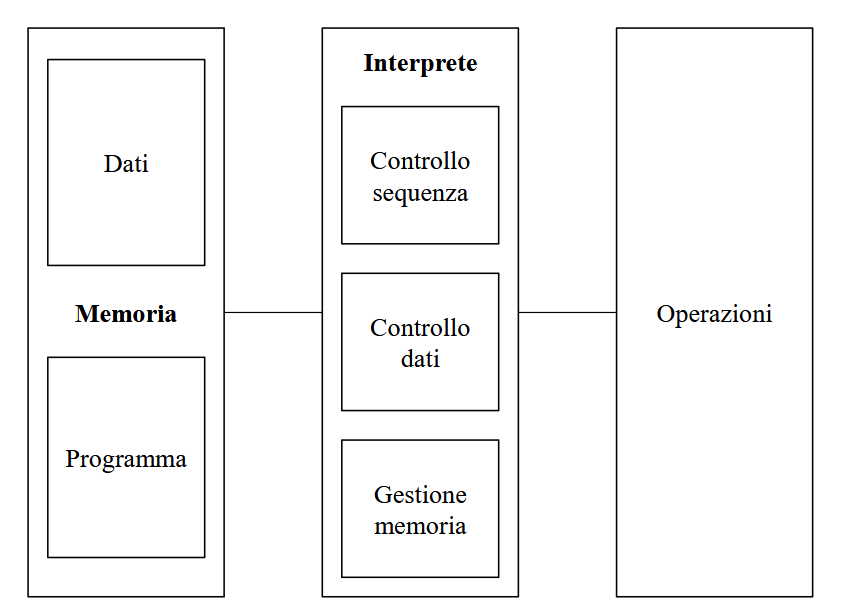
\includegraphics[width=0.75\textwidth]{macchina_astratta}
		\caption{La struttura di una macchina astratta}
	\end{figure}
	Come mostrato dalla figura, una generica macchina astratta è composta da una \textit{memoria} e da un \textit{interprete}.
	\subsection{L'Interprete}
	L'interprete dovrà compiere delle operazioni specifiche che dipendono dal linguaggio $\mathcal{L}$ che deve essere interpretato. Tuttavia, pur nella diversità dei linguaggi, ci sono delle operazioni comuni a tutti gli interpreti. Per quanto riguarda il tipo di operazioni che l'interprete esegue e le relative strutture dati individuiamo le seguenti categorie:
	\begin{itemize}
		\item operazione per l'elaborazione dei dati primitivi: servono per elaborare numeri interi, reali e/o operazioni aritmetiche;
		\item operazioni e strutture dati per il controllo della sequenza di esecuzione delle operazioni: servono per gestire il flusso di controllo delle istruzioni, strutture dati per memorizzare l'indirizzo della prossima istruzione e operazioni per manipolare le strutture dati;
		\item operazioni e strutture dati per il controllo del trasferimento dei dati: gestiscono il trasferimento dei dati dalla memoria all'interprete e viceversa e possono far uso di strutture dati ausiliari come la pila;
		\item operazioni e strutture dati per la gestione della memoria: queste sono relative all'allocazione di memoria per i dati e programmi.
	\end{itemize} 
	Vediamo il ciclo di esecuzione di un generico interprete:
	\begin{figure}[H]
		\centering
		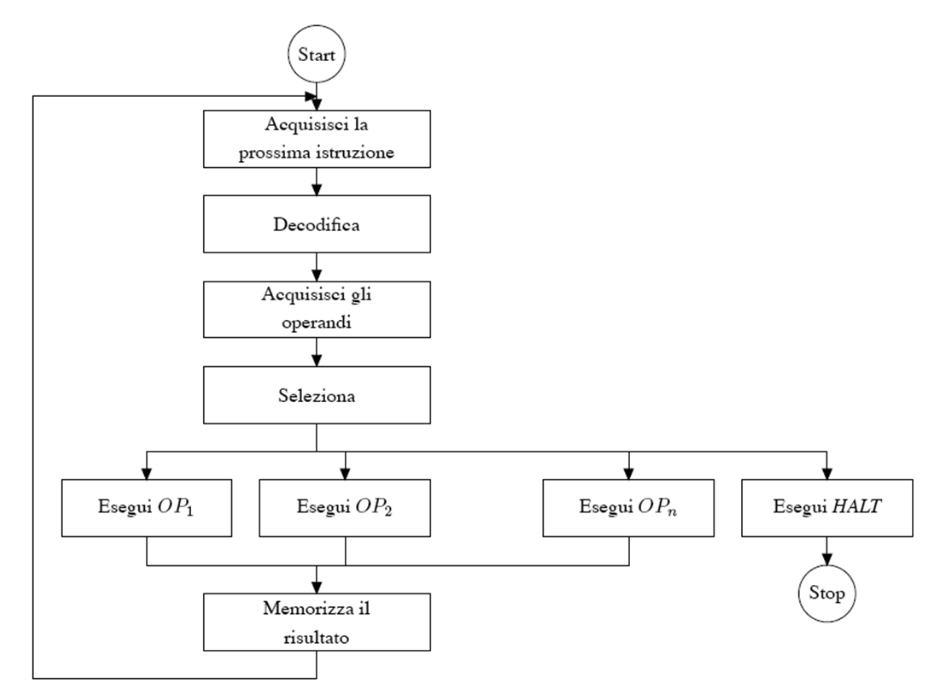
\includegraphics{ciclo_esecuzione_interprete}
		\caption{Ciclo di esecuzione di un generico interprete}
	\end{figure}
	\subsection{Realizzazione di una macchina astratta}
	{
		\definition[Linguaggio macchina]{Data una macchina astratta $\mathcal{M_L}$, il linguaggio $\mathcal{L}$ compreso dall'interprete di $\mathcal{M_L}$ è detto linguaggio macchina di $\mathcal{M_L}$}
	} \\
	Una qualsiasi macchina astratta $\mathcal{M_L}$ per essere effettivamente realizzata dovrà prima o poi utilizzare qualche dispositivo fisico per eseguire le istruzioni di $\mathcal{L}$. Oltre alla realizzazione fisica dei costrutti di $\mathcal{M_L}$ possiamo pensare a realizzazioni che usino invece livelli intermedi fra $\mathcal{M_L}$ e il dispositivo fisico di base e le possibili combinazioni sono:
	\begin{itemize}
		\item simulazione mediante software;
		\item emulazione mediante firmware, ovvero microprogrammi in linguaggi di basso livello.
	\end{itemize}
	Per quanto concerne la realizzazione mediante software, una macchina astratta $\mathcal{M_L}$ viene realizzata nel seguente modo:
	\begin{itemize}
		\item algoritmi e strutture dati di $\mathcal{M_L}$ vengono realizzati in un altro linguaggio $\mathcal{L'}$ già implementato;
		\item $\mathcal{M_L}$ è realizzata mediante programmi in $\mathcal{L'}$ che simulano le funzionalità di $\mathcal{M_L}$;
		\item $\mathcal{M_L}$ è realizzata attraverso la macchina $\mathcal{M'_L}$;
		\item $\mathcal{M'_L}$ è detta macchina \textit{ospite} e si denota con $\mathcal{M\text{o}_{L\text{o}}}$;
		\item l'implementazione di $\mathcal{L}$ sulla macchine ospite avviene mediante una qualche \textit{traduzione} di $\mathcal{L}$ in $\mathcal{L\text{o}}$;
		\item a seconda di come avviene la traduzione si parla di:
		\begin{itemize}
			\item \textbf{implementazione interpretativa};
			\item \textbf{interpretazione compilativa}
		\end{itemize}
	\end{itemize}
	\subsection{Funzioni parziali}
	Una funzione \textit{parziale}
	\[
	f: A \to B
	\]	
	è una corrispondenza tra elementi dell'insieme \textit{A} e quelli dell'insieme \textit{B} tale che , per ogni elemento di \textit{A} esiste uno ed uno solo elemento di \textit{B} che gli corrisponde e che chiamiamo $f(a)$. \\
	Una funzione \textit{parziale} è ancora una corrispondenza tra i due insiemi \textit{A} e \textit{B}. ma può essere indefinita in corrispondenza di qualche elemento del dominio \textit{A}. \\
	La nozione di funzione parziale è fondamentale per noi in quanto i programmi definiscono in modo naturale funzioni parziali, ad esempio:
	\begin{lstlisting}
read(x);
if x==1 then print(x) else
	while (x <> 1) do skip;
	\end{lstlisting}
	calcola la funzione parziale: 
	$f(x) = \begin{cases}
		1 \quad x=1 \\
		\text{indefinita} \quad \text{altrimenti}
	\end{cases}$
	In generale un programma scritto in $\mathcal{L}$ si può vedere come una funzione parziale:
	\[
	\mathcal{P^L}: \mathcal{D} \to \mathcal{D} \mid \mathcal{P^L}(Input) = Output
	\]
	se l'esecuzione di $\mathcal{P^L}$ sul dato di ingresso $Input$ termina e produce come risultato $Output$, mentre la funzione $\mathcal{P^L}$ non è definita se l'esecuzione di essa sul dato di ingresso $Input$ non termina.
	\subsection{Implementazione interpretativa pura}
	{
		\definition[Interprete]{Un interprete per il linguaggio $\mathcal{L}$, scritto nel linguaggio $\mathcal{Lo}$, è un programma che realizza la funzione parziale:
		\[
			\mathcal{I^{L\text{o}}_{L}}: (Prog^{\mathcal{L}} \times \mathcal{D}) \to \mathcal{D} \mid \mathcal{I^{L\text{o}}_{L}(P^L,}Input) = \mathcal{P^L}(Input)
		\]
		}
	}
	Nell'implementazione interpretativa pura di $\mathcal{L}$ non vi è una traduzione esplicita dei programmi scritti in $\mathcal{L}$, vi è solo un procedimento di decodifica dove l'interprete $\mathcal{I^{L\text{o}}_{L}}$, per eseguire un'istruzione di $\mathcal{L}$ la fa corrispondere un insieme di istruzioni di $\mathcal{L}o$. Questa decodifica non è una traduzione perchè il codice corrispondente viene eseguito direttamente e non prodotto in uscita.
	\subsection{Implementazione compilativa pura}
	Nell'implementazione \textit{compilativa pura} l'implementazione di $\mathcal{L}$ avviene traducendo esplicitamente i programmi scritti in $\mathcal{L}$ in $\mathcal{L}o$. In questo contesto $\mathcal{L}$ è detto \textit{linguaggio sorgente} e $\mathcal{L}o$ è detto \textit{linguaggio oggetto}. \\
	Per eseguire un programma $\mathcal{P^L}$ con un dato di input $\mathcal{D}$, dovremmo eseguire $\mathcal{C_{L,L\text{o}}}$ con $\mathcal{P^L}$. Questo produrrà come risultato un programma compilato $\mathcal{P\text{c}^{L\text{o}}}$ scritto in $\mathcal{L}o$. A questo punto potremo eseguire $\mathcal{P\text{c}^{L\text{o}}}$ sulla macchina $\mathcal{M}o_{\mathcal{L}o}$ con il dato di input $\mathcal{D}$ per ottenere il risultato desiderato. \\
	{
		\definition[Compilatore]{Un compilatore da $\mathcal{L}$ a $\mathcal{L}o$ è un programma che realizza una funzione: 
		\[
		\mathcal{C_{L,L\text{o}}}: Prog^{\mathcal{L}} \to Prog^{\mathcal{L}o}
		\]		
		tale che, dato un programma $\mathcal{P^L}$, se
		\[
		\mathcal{C_{L,L\text{o}}(P^L)} = \mathcal{P\text{c}^{L\text{o}}}
		\]
		allora per ogni $Input \in \mathcal{D}$
		\[
		\mathcal{P^L}(Input) = \mathcal{P\text{c}^{L\text{o}}}(Input)
		\]
		}
	}
	A differenza di quanto avviene con l'interpretazione, la fase di compilazione è separata dalla fase di esecuzione. La compilazione, infatti produce come risultato un programma che potremmo eseguire successivamente. 
	\paragraph{Confronto tra le due tecniche} \quad \\
	Analizziamo vantaggi e svantaggi delle due tecniche. Per quanto riguarda l'implementazione interpretativa pura lo svantaggio risiede nella scarsa efficienza. Infatti, dato che non vi è una fase preliminare di traduzione, per eseguire il programma $\mathcal{P^L}$ l'interprete $\mathcal{I^{L\text{o}}_{L}(P^L}$ deve effettuare al momento dell'esecuzione una decodifica dei costrutti del linguaggio $\mathcal{L}$. Quindi ai tempi richiesti dall'esecuzione dalle operazioni del programma si devono sommare anche i tempi necessari alla decodifica. Inoltre, l'interprete per ogni occorrenza di uno stesso comando nel programma l'interprete deve effettuare una nuova decodifica. \\
	Tuttavia, gli svantaggi in termini di efficienza vengono compensanti da vantaggi in termini di \textit{flessibilità}, infatti, interpretare al momento stesso dell'esecuzione i costrutti del programma che vogliamo eseguire permette di interagire in modo diretto con l'esecuzione del programma e questo è particolarmente importante per poter definire in modo semplice strumenti di debugging dei programmi. Inoltre, lo sviluppo di un interprete è più semplice dello sviluppo di un compilatore. \\
	Per quanto concerne l'implementazione compilativa pura, uno dei vantaggi riguarda una maggiore efficienza, in quanto uno stesso comando viene decodificato una sola volta indipendentemente da quante volte verrà eseguito, d'altra parte, però, uno degli svantaggi risiede nella \textit{perdita di informazioni} riguardo alla struttura del programma sorgente, il che rende più difficile l'interazione con il programma a tempo di esecuzione.
	\subsection{Gerarchia di macchine astratte}
	Ipotizziamo una gerarchia di macchine astratte come: $\mathcal{M_{L\text{0}}}, \mathcal{M_{L\text{1}}}, \dots, \mathcal{M_{L\text{n}}}$. \\
	$\mathcal{M_{L\text{i}}}$ è implementata sfruttando il linguaggio della macchina sottostante $\mathcal{M_{L\text{i - 1}}}$ e analogamente, $\mathcal{M_{L\text{i}}}$ fornisce il proprio linguaggio alla macchina sovrastante. \\
	Inoltre, c'è indipendenza tra i livelli, infatti, modifiche interne alle funzionalità di un livello non hanno influenza sugli altri livelli. 
	\begin{figure}[H]
		\centering
		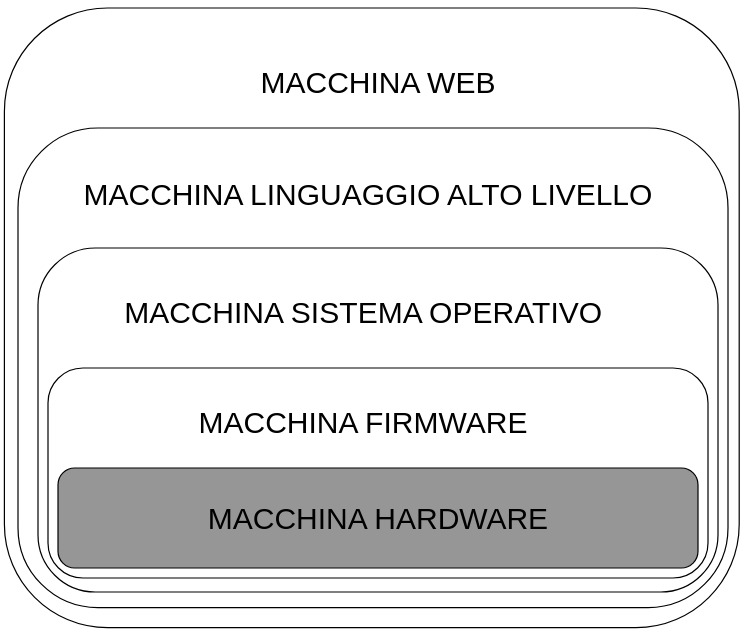
\includegraphics[width=0.7\textwidth]{gerarchia_macchine_astratte}
	\end{figure}
	\section{Programmi e funzioni calcolabili}
	In questa sezione verranno trattate le limitazioni dei programmi che si possono scrivere con i linguaggi di programmazione e vedremo se ci sono dei problemi che non possono essere risolti e capiremo se la risposta a questo quesito dipende dal linguaggio di programmazione utilizzato.
	\subsection{Il problema della fermata}
	Una funzione parziale $f: A \to B$ è calcolabile nel linguaggio $\mathcal{L}$ se esiste un programma $\mathcal{P}$ scritto in $\mathcal{L}$ tale che se $f(a) = b$ allora $\mathcal{P}(a)$ termina e produce come output $b$ altrimenti $\mathcal{P}(a)$ non è definita e va in ciclo.  \\
	Quindi il quesito che ci siamo posti precedentemente riguardo l'esistenza di problemi per i quali non esiste un programma che li risolva riguarda, ora, l'esistenza di funzioni \textbf{non calcolabili}.  \\
	Allora, vogliamo stabilire se un programma termina su un dato input. \\
	Definiamo quindi con $\mathcal{H}$, un programma di debugging, che riceve in ingresso due input: un generico programma $\mathcal{P}$ scritto nel linguaggio $\mathcal{L}$ e un generico input $x$ per tale programma: \\
	\begin{lstlisting}
Boolean H(P, x):
	boolean term;
	if (P(x) termina)
	 	then term = true;
	else 
		term = false;
	return term;
	\end{lstlisting}
	Quindi $\mathcal{H(P}, x)$ ritorna \textit{true} se $\mathcal{P}(x)$ termina e \textit{false} se quest'ultimo va in loop. \\
	Sottolineiamo come $H$ deve terminare sempre e deve funzionare per ogni programma $\mathcal{P^L}$ e ogni input $x$. \\
	Adesso vogliamo dimostrare che non esista alcun programma $\mathcal{H}$ con il comportamento descritto precedentemente. Dimostreremo questo per assurdo, quindi supponendo di avere a disposizione $\mathcal{H}$ e di ricavarne una contraddizione. \\
	Sfruttando $\mathcal{H}$ possiamo scrivere un altro programma $K$, con un solo input che si tratta di un generico programma $\mathcal{P}$:
	\begin{lstlisting}
	if (H(P, P) = false) then print("LOOP");
		else while (true) do print("TERMINA");
	\end{lstlisting}
	Quindi $K$ è la negazione di H, infatti, termina se $P(P)$ non termina e va in loop se $P(P)$ termina. \\
	Eseguiamo ora $K$ sul suo stesso testo, ovvero $K(K)$, il comportamento che si ottiene è il seguente:
	\[
	K(K) = \begin{cases}
		TERMINA \quad K(K) \ \text{non termina} \\
		LOOP \quad K(K) \ \text{termina}
	\end{cases}
	\]
	Ma questo è assurdo perchè $K(K)$ termina se $K(K)$ non termina; e che non termina, quando $K(K)$ termina. \\
	L'assurdo dipende, non da $K$ in se, che è un semplice programma che sfrutta $H$, ma l'assurdo discende dall'aver supposto che esistesse un programma con le caratteristiche di $H$. Quindi $H$ non esiste. \\
	Il problema della fermata è \textbf{indecidibile}, cioè non possiamo costruire un algoritmo che lo risolva, quindi, per rispondere al quesito riguardante l'esistenza di funzioni non calcolabili, la risposta è si e il problema della fermata è un esempio di queste e questo risultato non dipende dal linguaggio $\mathcal{L}$ utilizzato.
	\section{Macchine di Turing}
	Vedere dalle slide
	\section{Introduzione alla teoria dei linguaggi formali}
	Un linguaggio di programmazione è un formalismo artificiale nel quale poter esprimere algoritmi. Il suo studio può far tesoro di alcuni concetti e strumenti sviluppati nell'ultimo secolo dalla linguistica. 
	\subsection{Livelli di descrizione}
	Nella descrizione di un linguaggio si individuano tre grandi ambiti: quello della \textit{grammatica}, quello della \textit{semantica} e quello della \textit{pragmatica}. \\
	La \textit{grammatica} risponde alla domanda "Quali frasi sono corrette?" Una volta che sia definito l'alfabeto del linguaggio ad un primo stadio, quello \textit{lessicale}, utilizzando questo alfabeto, sono individuate le sequenza corrette di simboli che costituiscono le \textit{parole} del linguaggio. Definiti alfabeto e parole, la \textit{sintassi} descrive quali sequenza di parole definiscono frasi legali. La sintassi è una relazione tra segni, tra tutte le possibili sequenze di parole, seleziona un sottoinsieme di sequenza che costituiscono le frasi del linguaggio stesso. \\
	La \textit{semantica} cerca di dare la risposta alla domanda: "Cosa significa frase corretta?" La semantica, dunque, attribuisce un \textit{significato} ad ogni frase corretta. \\
	Al terzo livello, entra in scena l'attore principale, colui che usa un certo linguaggio. La \textit{pragmatica}, si chiede "Come usare una frase corretta e sensata?" Frasi con lo stesso significato possono essere utilizzate in modo diverso da utenti diversi. \\
	Nel caso dei linguaggi di programmazione, a questi tre livelli, se ne aggiunge un quarto, quello dell'\textit{implementazione}, quindi "Come eseguire una frase corretta, in modo da rispettarne la semantica?"
	\subsection{Grammatica e sintassi}
	La grammatica di un linguaggio stabilisce prima alfabeto e lessico, e quindi, definisce, con la sintassi, quali sequenza di simboli corrispondano a frasi ben formato. \\
	Esistono due tipologie di grammatiche:
	\begin{enumerate}
		\item \textbf{regolari};
		\item \textbf{libere da contesto}.
	\end{enumerate}
	L'informatica teorica è la \textbf{scienza degli algoritmi}, in tutti i loro aspetti, poichè è il concetto dell'algoritmo che è comune a tutti i settori dell'informatica. \\
	\begin{figure}[H]
		\centering
		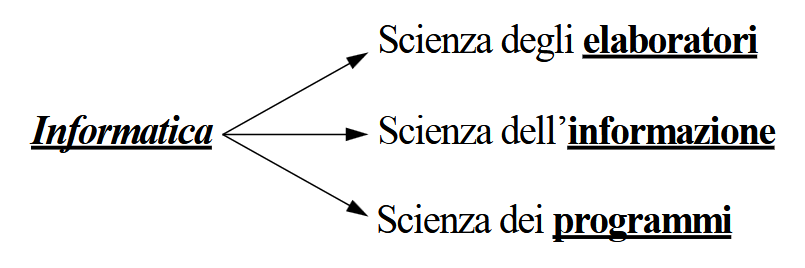
\includegraphics[width=1.00\textwidth]{settori_informatica}
	\end{figure} 
	Gli \textbf{elaboratori} sono macchine che eseguono gli algoritmi, l'\textbf{informazione} è la materia sulla quale lavorano gli algoritmi e i \textbf{programmi} sono gli algoritmi descritti in un particolare linguaggio. \\
	\begin{figure}[H]
		\centering
		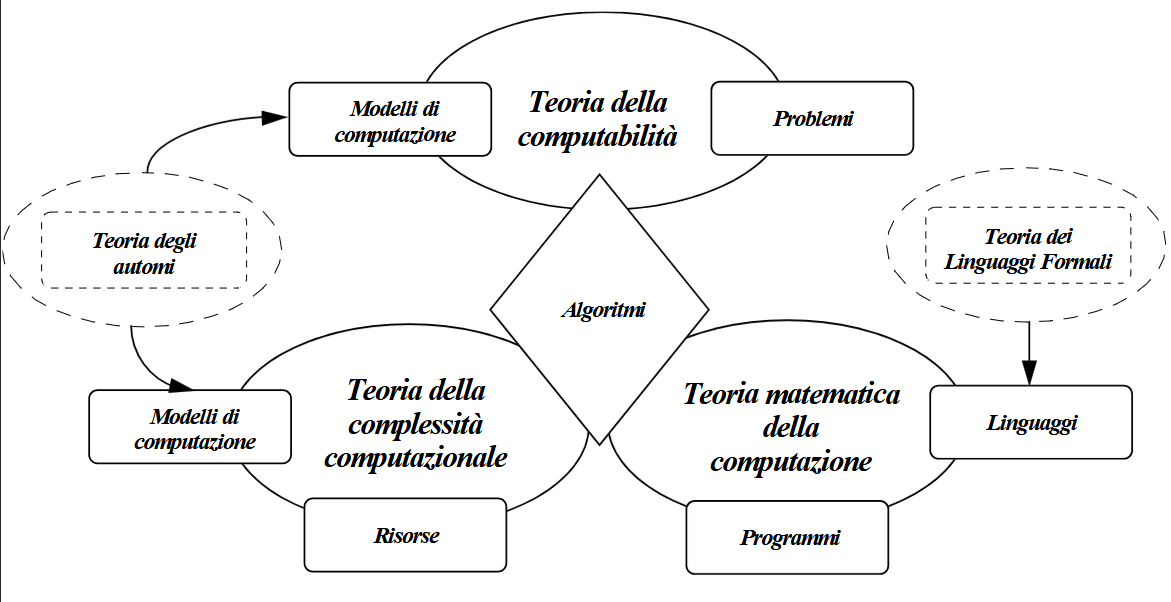
\includegraphics[width=1.00\textwidth]{area_ricerca_informatica_teorica}
	\end{figure}
	Questo schema fornisce una panoramica delle aree di ricerca che ricadono nell'ambito più generale dell'informatica teorica. Queste aree sono:
	\begin{itemize}
		\item \textbf{teoria della computabilità}: essa si occupa dell'esistenza o meno di algoritmi risolutivi di problemi con un determinato modello di computazione, ovvero una macchina astratta. La teoria della computabilità è legata alla \textbf{teoria degli automi} che si occupa della definizione di diverse classi di dispositivi di calcolo e, per ogni classe, dello studio delle proprietà e delle classe di problemi che sono in grado di risolvere. In questa area di ricerca, lavorano più matematici e meno informatici. \\
		Particolarmente produttiva, si è rivelata l'interazione tra la \textit{teoria degli automi} e la \textit{teoria dei linguaggi formali}, in quanto quest'ultima è stata sviluppata e utilizzata dagli informatici teorici in quanto avevano bisogno di descrivere gli algoritmi con linguaggi di programmazione comprensibili dalla macchine, ma non troppo difficili per l'uomo e \textbf{non ambigui}. 
		\item \textbf{teoria matematica della computazione}: è il rapporto tra gli algoritmi e i linguaggi di programmazione ed indica la proprietà dei programmi quali correttezza, completezza e terminazione.
		\item \textbf{teoria delle complessità computazionale}: è il rapporto tra gli algoritmi e le risorse necessarie per eseguirli. Questa è una branca della teoria della computabilità che studia le risorse minime necessarie per la risoluzione di un problema. Inoltre, indica gli aspetti quantitativi del procedimento di soluzione di un problema.
	\end{itemize}
	\subsection{Studio dei linguaggi}
	Come sappiamo, i linguaggi di programmazione vengono usati per scrivere programmi e quindi per comunicare con il computer che sono limitati a comprendere il significato desiderato dei programmi. \\
	In un linguaggio naturale possiamo anche comunicare attraverso frasi mal strutturate e incomplete ma con il computer non è cosi. \\
	I nostri programmi devono aderire rigorosamente a regole stringenti e anche differenze minori vengono rigettate come errate. Ogni frase in un linguaggio dovrebbe essere corretta sia \textbf{semanticamente}, ovvero avere il corretto significato, sia \textbf{sintatticamente} cioè avere la corretta struttura grammaticale. In programmazione, è essenziale che la \textbf{sintassi} sia corretta al fine di comunicare una qualsivoglia semantica. Quindi la sintassi è una \textbf{condizione necessaria} per la semantica ed essa è una \textbf{condizione sufficiente} per la sintassi.
	\paragraph{Sintassi e semantica} \quad \\
	Lo studio della sintassi è lo studio della grammatica, cioè della struttura delle frasi. La frase:
	\[
	The\ man\ hits\ the\ dog
	\]
	può essere analizzata sintatticamente, cioè risolta nelle parti grammaticali componenti, come segue:
	\begin{itemize}
		\item \textit{the man}, la parte nominale;
		\item \textit{hits}, la parte verbale;
		\item \textit{the dog}, la parte nominale.
	\end{itemize}
	ed ogni frase in questa forma è sintatticamente valida in inglese. Quindi, possiamo descrivere un particolare insieme di tali frasi semplici in inglese usando le seguenti regole:
	\begin{itemize}
		\item $<$ frase semplice $>$ ::= $<$ parte nominale $>$ $<$ parte verbale $>$ $<$ parte nominale $>$ 
		\item $<$ parte nominale $>$ ::= $<$ articolo $>$ $<$ nome $>$
		\item $<$ nome $>$ ::= \textbf{$\textit{car}|\textit{man}|\textit{dog}$}
		\item $<$ articolo $>$ ::= \textbf{$\textit{The}|\textit{a}$}
		\item $<$ parte verbale $>$ ::= \textbf{$\textit{hits}|\textit{eats}$}
	\end{itemize}
	Queste regole sono scritte in \textbf{BNF}, Backus Naur Form, un metalinguaggio comunemente usato per descrivere la sintassi dei linguaggi di programmazione. \\
	Tutto ciò si può riassumere nel seguente \textbf{albero di derivazione}:
	\begin{figure}[H]
		\centering
		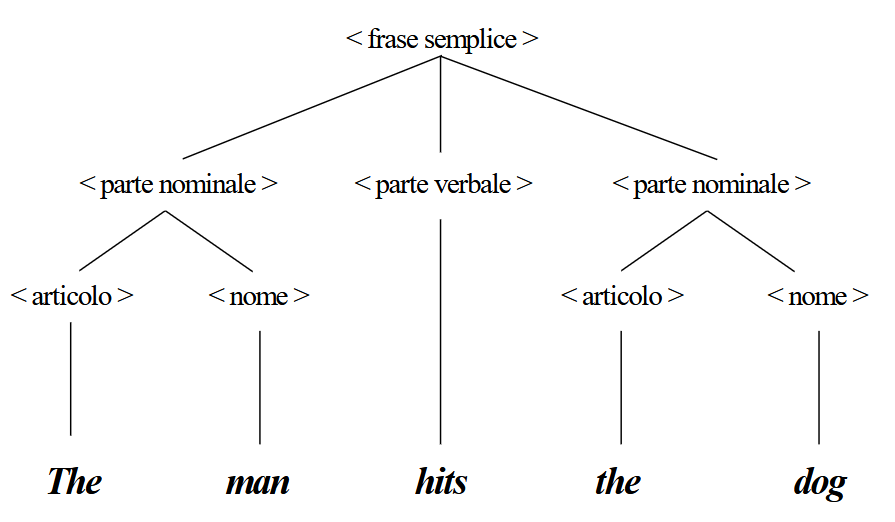
\includegraphics[width=1.00\textwidth]{albero_di_derivazione}
	\end{figure}
	La definizione data di $<$frase semplice$>$ dà luogo a 72 diverse frasi derivabili, sebbene siano tute sintatticamente corrette, in base alla nostra definizione, alcune non hanno un'interpretazione semantica sensata, come ad esempio \textit{The car eats the man}. \\
	Consideriamo la seguente frase, non derivabile da $<$frase semplice$>$:
	\[
	They\ are\ flying\ planes
	\]
	Un'analisi sintattica di questa frase è:
	\begin{itemize}
		\item \textit{They}: pronome;
		\item \textit{are}: verbo;
		\item \textit{flying planes}: parte nominale dove \textit{flying} è l'aggettivo e \textit{planes} è il nome.
	\end{itemize}
	Quest'analisi suggerisce che \textit{they} si riferisce a \textit{planes}, ovvero \textit{aerei nel cielo che volano}. Un'analisi alternativa sarebbe:
	\begin{itemize}
		\item \textit{they}: pronome;
		\item \textit{are flying}: verbo;
		\item \textit{planes}: nome.
	\end{itemize}
	Questa implicherebbe un'interpretazione semantica completamente differente, in cui \textit{they} si riferisce a chiunque sia al controllo dei \textit{planes}, ovvero \textit{essi stanno pilotando degli aerei}. \\
	In questo esempio, l'analisi sintattica è di aiuto all'interpretazione semantica e per quanto sia scelto ad hoc e mostri un fenomeno poco comune nel linguaggio naturale, l'esempio è illustrativo di un concetto importante in computazione. Una fase cruciale nel processo di compilazione di un programma è l'\textbf{analisi sintattica}, come passo essenziale per la sua \textbf{interpretazione semantica}. \\
	\paragraph{Teoria dei linguaggi formali} \quad \\
	Negli anni '50, Noam Chomsky, un linguista americano cerca di descrivere la sintassi del linguaggio naturale secondo semplici \textbf{regole di riscrittura} e \textbf{trasformazione}. Chomsky considera alcune \textbf{restrizioni} sulle regole sintattiche e classifica i linguaggi in base alle restrizione imposte alle regole che generano tali linguaggi. \\
	Una classe importante di regole che generano linguaggi formali che generano linguaggi formali va sotto il nome di \textbf{grammatiche libere da contesto} o \textbf{Context-free grammars} (C.F). \\
	Questa classe è molto importante in quanto lo sviluppo dei primi linguaggi di programmazione di alto livello, che segue di pochi anni il lavoro di Chomsky, dimostra che le grammatiche C.F sono strumenti adeguati a descrivere la sintassi di base di molti linguaggi di programmazione. \\
	Un linguaggio C.F è il linguaggio delle parentesi ben formate che comprende tutte le stringhe di parentesi aperte e chiuse bilanciate correttamente, ad esempio:
	\begin{itemize}
		\item () è ben formata;
		\item (()()) è ben formata;
		\item (()() non è ben formata.
	\end{itemize}
	Questo linguaggio è fondamentale in informatica nelle definizioni delle espressioni. \\
	\textbf{Definizione}:
	\begin{itemize}
		\item La stringa () è ben formata;
		\item se la stringa di simboli \textit{A} è ben formata allora lo è anche (A);
		\item se le stringhe \textit{A} e \textit{B} sono ben formate, allora lo è anche la stringa \textit{AB}.
	\end{itemize}
	In corrispondenza di questa definizione induttiva, possiamo considerare un sistema di riscrittura che genera esattamente l'insieme delle stringhe lecite di parentesi ben formate:
	\begin{enumerate}
		\item S $\to$ ();
		\item S $\to$ (S);
		\item S $\to$ SS
	\end{enumerate}
	Le regole di riscrittura 1,2,3 sono dette \textbf{produzioni} o \textbf{regole di produzione}. \\
	\textbf{Esempio: generazione di (())(()())}:
	\begin{itemize}
		\item \textbf{primo modo}: \\
			\begin{figure}[H]
				\centering
				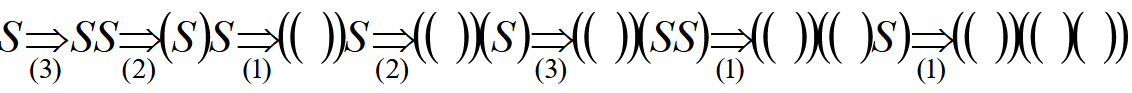
\includegraphics[width=1.0\textwidth]{esempio_derivazione_1}
			\end{figure}
			La corrispondente sequenza di applicazione delle produzioni è: $3 \to 2 \to 1 \to 2 \to 3 \to 1 \to 1$
		\item \textbf{secondo modo}:
		\begin{figure}[H]
			\centering
			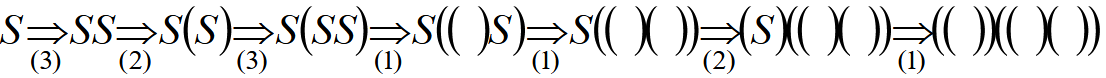
\includegraphics[width=1.00\textwidth]{esempio_derivazione_2}
		\end{figure}
		La corrispondete sequenza di applicazione delle produzioni è: $3 \to 2 \to 3 \to 1 \to 1 \to 2 \to 1$ \\
		Una sequenza di applicazione di regole di produzione prende il nome di \textbf{\textit{derivazione}}.
	\end{itemize}
	Nei due esempi precedenti abbiamo utilizzato la notazione:	
	\begin{align*}
		\alpha \underset{(n)}{\Rightarrow} \beta 
	\end{align*}
	e si legge: "da $\alpha$ si produce direttamente $\beta$ per effetto dell'applicazione della regola di riscrittura $n$", per l'esempio precedente possiamo scrivere:
	\begin{align*}
		S \overset{*}{\Rightarrow} (())(()())
	\end{align*}
	che leggiamo come "S produce (())(()())". \\
	Nelle regole di produzione si è fatto uso di due tipi di simboli: caratteri che possono apparire nelle derivazioni, ma non nelle stringhe finali, detti \textbf{simboli nonterminali} o \textbf{variabili}, come ad esempio il carattere $S$ dell'esempio precedente, e caratteri che possono apparire nelle stringhe finali, detti \textbf{simboli terminali}. \\
	In BNF si usa la seguente notazione: 
	\begin{align*}
		\underset{\to}{S} \quad \underset{::=}{<S>}
	\end{align*}
	\chapter{Grammatiche e linguaggi}
	\section{Linguaggi formali e monoidi liberi}
	Il concetto di \textit{linguaggio formale} è strettamente correlato a quello di \textit{monoide libero}, ovvero generato da un insieme. \\
	{
		\definition[Alfabeto]{Un insieme $X$ finito e non vuoto di simboli è un \textit{\textbf{alfabeto}}}
	}
	{
		\definition[Parola o Stringa]{Una sequenza finita di simboli $x_1x_2\dots x_n$, dove ogni $x_i$ è preso da uno stesso alfabeto $X$ è una \textit{\textbf{parola}} su $X$}
	}
	Ad esempio:
	\begin{itemize}
		\item $X = \{0, 1\}$
		\item $001110$ è una parola su $X$.
	\end{itemize}
	Quindi, una parola è ottenuta concatenando simboli dell'alfabeto. Se una stringa ha $m$ simboli, non necessariamente distinti allora la stringa avrà lunghezza $m$. \\
	La lunghezza di una stringa $w$ è denotata con $|w|$, nell'esempio precedente $001110$ è una stringa di lunghezza 6. \\
	La parola vuota, denotata con $\lambda$, è una stringa priva di simboli ed ha lunghezza 0.
	\[
	|\lambda| = 0
	\]
	{
		\definition[Uguaglianza tra stringhe]{Due stringhe sono uguali se i loro caratteri, letti ordinatamente da sinistra a destra, coincidono}
		\definition[$X^*$]{L'insieme di tutte le stringhe di lunghezza finita su l'alfabeto $X$ si denota con $X^*$}
	}
	Ad esempio:
	\begin{itemize}
		\item $X = \{0, 1\}$
		\item $X^* = \{\lambda, 0, 1, 00, 01, 10, 11, \dots\}$
	\end{itemize}
	$X^*$ ha un numero di elementi che è un infinito numerabile, quindi da questo segue che $\lambda \in X^*\ \forall\ insieme\ X$
	{
		\definition[Concatenazione o prodotto]{Sia $\alpha \in X^*$ una stringa di lunghezza $m$ e $\beta \in X^*$ una stringa di lunghezza $n$, la concatenazione di $\alpha$ e $\beta$, denotata con $\alpha\beta$ o $\alpha \cdot \beta$, è definita come la stringa di lunghezza $m + n$, i cui primi $m$ simboli costituiscono una stringa uguale ad $\alpha$ e gli ultimi $n$ simboli costituiscono una stringa uguale a $\beta$}
	}
	Quindi se $\alpha = x_1x_2\dots x_m$ e $\beta = x_1'x_2'\dots x_n'$ si ha:
	\[
	\alpha\beta = x_1x_2\dots x_mx_1'x_2'\dots x_n'
	\]
	La concatenazione di stringhe su $X$ è una operazione binaria su $X^*$:
	\[
	\cdot: X^* \times X^* \to X^*
	\]
	\begin{itemize}
		\item è \textbf{associativa}: $(\alpha\beta)\gamma=\alpha(\beta\gamma) \quad \forall \alpha, \beta, \gamma \in X^*$
		\item \textbf{non è commutativa}: $\exists \alpha, \beta \in X^* \mid \alpha\beta \neq \beta\alpha$
		\item \textbf{ha elemento neutro $\lambda$}:	 $\lambda\alpha=\alpha\lambda=\alpha \quad \forall \alpha \in X^*$
	\end{itemize}
	Dunque $(X^*, \cdot)$ \textbf{è un monoide non commutativo}. \\
	In base alla definizione di prodotto, ogni parola non vuota $\alpha=x_1x_2\dots x_n$, si può scrivere in uno ed un solo modo come prodotto di parole di lunghezza 1, cioè elementi di $X$, quindi il confronto fra due parole avviene confrontando i singoli caratteri che compongono le stringhe, secondo la relazione data nella definizione dell'alfabeto, ad esempio se $X = \{a, b\}$ e $a < b$ allora $aa < ab$. \\
	Questo si esprime dicendo che:
	\begin{itemize}
		\item $(X^*, \cdot)$ è il monoide libero generato dall'insieme $X$.
	\end{itemize}
	{
		\definition[Prefisso, Suffisso]{Se $\gamma \in X^*$ è della forma $\gamma = \alpha\beta$, ove $\alpha, \beta \in X^*$, allora $\alpha$ è un \textit{prefisso} di $\gamma$ e $\beta$ è un \textit{suffisso} di $\gamma$}
		\definition[Sottostringa]{Se $\delta, \beta \in X^*$ e $\delta$ è della forma $\delta=\alpha\beta\gamma$, ove $\alpha,\gamma \in X^*$ allora $\beta$ è una sottostringa di $\delta$}
	}
	Ad esempio:
	\begin{itemize}
		\item Sia $\gamma = 00110$. Allora:
		\item $\{\lambda, 0, 00, 001, 0011, \gamma\}$ è l'insieme dei prefissi di $\gamma$
		\item $\{\lambda, 0, 10, 110, 0110, \gamma\}$ è l'insieme dei suffissi di $\gamma$
		\item $\{\lambda, 0, 1, 00, 01, 11, 001, 011, 110, 0011, 0110, \gamma\}$ è l'insieme delle sottostringhe di $\gamma$
	\end{itemize}
	{
		\definition[Potenza di una stringa]{Data una striga $\alpha$ su $X$, la potenza h-esima di $a$ è definita induttivamente come segue:
		\[
		\alpha^h = \begin{cases}
			\lambda \quad \quad \quad  h = 0 \\
			\alpha\alpha^{h-1} \quad \text{altrimenti}
		\end{cases}
		\]
		con $h=0,1,2, \dots$
		}
	} \\
	La potenza h-esima di una stringa è un caso speciale di concatenamento in quanto la si ottiene concatenando una stringa $h$ volte con se stessa.
	{
		\definition[Potenza di un alfabeto]{
			Sia $X$ un alfabeto, poniamo:
			\begin{enumerate}
				\item $X^1 = X$
				\item $X^2 = \{x_1x_2 \mid x_1,x_2 \in X, x_1x_2 \equiv x_1 \cdot x_2\}$
				\item $X^3 = \{x_1x_2x_3 \mid x_1x_2 \in X^2, x_3 \in X, x_1x_2x_3 \equiv x_1x_2 \cdot x_3\}$
				\item \dots
				\item $X^i = \{x_1\dots x_{i-1}x_i \mid x_1\dots x_{i - 1} \in X^{i - 1}, x_1 \in X, x_1\dots x_i \equiv x_1 \dots x_{i-1} \cdot x_i\}$
			\end{enumerate}
		}
	}
	Se $i \geq 2$ si ha: 
	\[
	X^+ = X \cup X^2 \cup \dots \cup X^i = \bigcup_{i=1}^{+\infty}X^i
	\]
	Se $\lambda$ è la parola vuota e prendiamo un $w \in X^+$ tale che $w \cdot \lambda = \lambda \cdot w= w$ si ha:
	\[
	X^* = \{\lambda\} \cup X^+
	\]
	$X^*$ si chiama \textit{chiusura riflessiva transitiva} di $X$. \\
	Inoltre, si ha:
	\[
	X^h = \begin{cases}
		\{\lambda\} \quad \quad \quad h=0 \\
		XX^{h-1} \quad \text{altrimenti}
	\end{cases}
	\]
	{
		\definition[Linguaggio formale]{Un \textit{linguaggio formale L} su un alfabeto \textit{X} è un sottoinsieme di $X^*$
		\[
		L \subseteq X^*
		\]
		}
	}
	Ad esempio:
	\begin{itemize}
		\item Il linguaggio delle parentesi ben formate è un linguaggio formale in quanto, denotato con $M$ tale linguaggio si ha: \[
			M \subset \{(,)\}^*
		\]
	\end{itemize}
	I linguaggi formali possono essere di natura molto diversa l'uno dall'altro. \\
	Un linguaggio di programmazione può essere costruito a partire dall'alfabeto $X$ dei simboli sulla tastiera. \\
	L'insieme, finito o infinito, dei programmi ben costruiti sintatticamente costituisce un linguaggio. \\
	Consideriamo l'insieme dei teoremi di una teoria matematica. I teoremi sono particolari stringhe di simboli del nostro alfabeto. L'insieme dei teoremi ben formati rappresenta un linguaggio. Ad esempio, la stringa $ab=ba$ non è un teorema della teoria dei gruppi, ma della teoria dei gruppi abeliani.
	\section{Generazione e riconoscimento di linguaggi formali}
	A noi interessano i linguaggi formali da 2 punti di vista:
	\begin{itemize}
		\item \textbf{Descrittivo o Generativo}
		\item \textbf{Riconoscitivo}
	\end{itemize}
	\subsection{Generazione dei linguaggi formali}
	Come possiamo generare gli elementi di un dato linguaggio $L$? Un linguaggio \textit{finito} può essere generato per \textit{estensione}, ossia per elencazione degli elementi. Un linguaggio \textit{infinito} non è elencabile. Questi sono i più interessanti perchè devono essere specificati necessariamente attraverso una \textit{proprietà} che ne caratterizza gli elementi, che ne definisce l'\textit{intensione}. Tale proprietà può essere vista come una regola da seguire per generare gli elementi del linguaggio. Il vero problema è trovare la/e regola/e generativa/e di un linguaggio in quanto non  è possibile memorizzare tutte le frasi del linguaggio. \\
	Ad esempio:
	\begin{itemize}
		\item Non è possibile elencare tutti i teoremi della teoria dei gruppi, perchè sono infiniti teoremi realizzabili combinando quelli noti.
		\item Un libro di teoria dei gruppi non è l'elencazione dei teoremi, ma fornisce una serie di assiomi e le regole con le quali, a partire dagli assiomi, è possibile costruire tutti i teoremi della teoria dei gruppi. 
	\end{itemize}
	Nel nostro caso, per descrivere la regola di produzione di un linguaggio, utilizzeremo una notazione insiemistica, ad esempio, sia $L$ il linguaggio su 
	$X = \{0\}$ costituito da tutte e sole le stringhe che hanno un numero pari di 0, cioè: 
	\[
	L = \{\lambda, 00, 0000, 000000, \dots\}
	\]
	La regola di produzione di $L$ viene espressa come segue: 
	\[
	L = \{\lambda\} \cup \{w^n \mid w = 00, n = 1,2, \dots\}
	\]
	che può essere semplificata come: $L = \{00\}^*$
	\subsection{Riconoscimento dei linguaggi formali} 
	Come possiamo riconoscere gli elementi di un dato linguaggio $L$? Questo secondo punto di vista ha come obiettivo la costruzione di "macchine" in grado di decidere/stabilire se una stringa è un elemento di $L$ oppure no. Si intende costruire una macchinetta cui dare in ingresso una data parola e che produce una tra due possibili risposte: $si \equiv \in L$ e $no \equiv \notin L$. \\
	\begin{figure}[H]
		\centering
		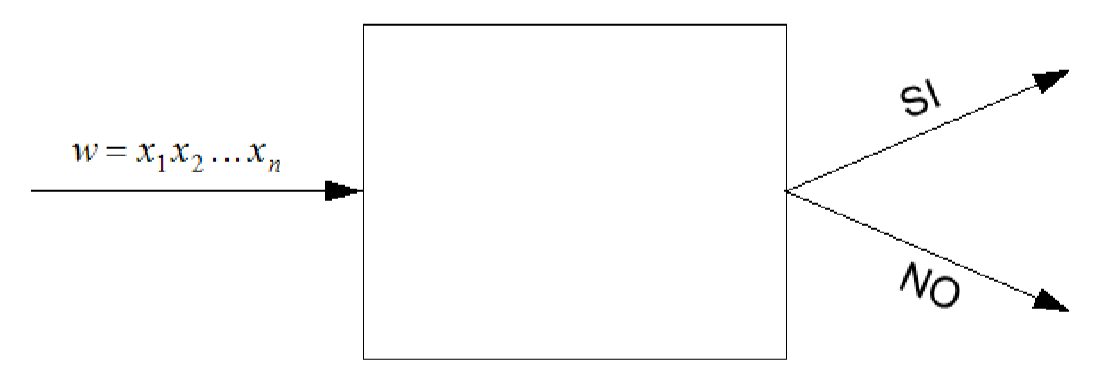
\includegraphics[width=1.00\textwidth]{riconoscimento_linguaggio}
	\end{figure}
	Ad esempio, l'esecuzione di un programma errato sintatticamente viene inibita. Questo è indice dell'esistenza di una macchinetta che stabilisce se il programma appartiene o no all'insieme dei programmi sintatticamente ben costruiti. \\
	Sia dato l'alfabeto: $X = \{0, 1, 2, 3, 4, 5, 6, 7, 8, 9, +, -\}$. \\
	Voglio generare il linguaggio $L$ dei numeri interi relativi. Ovviamente: $L \subseteq X^*$. \\
	Più precisamente, $L \subset X^*$ poichè ad esempio: $1++-5 \notin L$. \\
	Non possiamo elencare gli elementi di $L$, pertanto dobbiamo cercare una serie di regole mediante le quali è possibile produrre tutti e soli gli elementi di $L$. \\
	Assumiamo, per semplicità, che un numero relativo sia costituito da una serie di cifre precedute da + o -. \\
	Le produzione, scritte in BNF, sono:
	\begin{itemize}
		\item $< S > ::= + < I > | - < I >$
		\item $< I > ::= < D > | < I >< D >$
		\item $< D > ::= 0|1|2|3|4|5|6|7|8|9$
	\end{itemize}
	Queste regole generano tutti gli interi relativi purchè partiamo dal simbolo nonterminale $S$. \\
	$I$ è simbolo nonterminale, abbreviato $NT$, anche detto \textit{categoria sintattica}, che sta ad indicare e da cui si genera la classe dei numeri interi. \\
	$I$ è definito ricorsivamente o come una cifra oppure come un intero seguito da una cifra. \\
	Ogni intero relativo è generato da queste regole e niente che non sia un intero relativo può essere generato da queste regole. \\
	Dagli esempi visti, possiamo trarre le seguenti conclusioni. Per generare un linguaggio sono necessari:
	\begin{itemize}
			\item un insieme $X$ di simboli primitivi con cui si formano le parole del linguaggio, detto \textit{alfabeto dei simboli terminali} o \textit{alfabeto terminale}
			\item un insieme $V$ di simboli ausiliari o variabili con cui si identificano le categorie sintattiche del linguaggio, detto \textit{alfabeto dei simboli nonterminali} o \textit{alfabeto nonterminale} o \textit{alfabeto delle variabili}
			\item un simbolo speciale $S$, scelto tra i nonterminali, da cui far partire la generazione delle parole del linguaggio. Tale simbolo è detto \textit{assioma} o \textit{scopo} o \textit{simbolo distintivo} o \textit{simbolo di partenza} o \textit{simbolo iniziale}
			\item un insieme $P$ di \textit{produzioni}, espresse in un formalismo quali regole di riscrittura, BNF (a ::= b), carte sintattiche, ...
	\end{itemize}
	\section{Definizione di Grammatica generativa o a struttura di frase o a forma di frase}
	{
		\definition[Grammatica generativa]{
			Una \textit{\textbf{grammatica generativa}} o \textit{a struttura di frase G} è una quadrupla:
			\[
			G = (X, V, S, P)
			\]
			ove:
			\begin{itemize}
				\item $X$ è l'\textit{alfabeto terminale} per la grammatica;
				\item $V$ è l'\textit{alfabeto nonterminale} o delle variabili per la grammatica;
				\item $S$ è il \textit{simbolo di partenza} per la grammatica;
				\item $P$ è l'insieme delle \textit{produzioni} della grammatica
			\end{itemize}
			e inoltre valgono le seguenti condizioni:
			\[
			X \cap V = \emptyset \quad S \in V
			\]
		}
		\definition[Produzione]{Una \textit{produzione} è una coppia $(v, w)$ ove $v \in (X \cup V)^+$ e $v$ ha come sottostringa un $NT \iff v \in (X \cup V)^*V(X \cup V)^*$ e $w \in (X \cup V)^*$ dove $w$ può essere anche $\lambda$. \\
		Un elemento di $P$ viene comunemente scritto nella forma:
		\[
		v \to w
		\]
		e una produzione deve, in qualche modo, riscrivere un $NT$.
		} 
	} \\
	\textbf{Esempio di una grammatica}: la grammatica per il linguaggio delle parentesi ben formate è la seguente:
	\[
	G = (\{(,)\}, \{S\}, S, \{S \to (), S \to (S), S \to SS\})
	\] 
	La grammatica per il linguaggio dei numero interi relativi è la seguente:
	\[
	G = (\{0, \dots, 9, +, -\}, \{S, I, D\}, S, \{S \to +I, S \to -I, I \to D, I \to ID, D \to 0, \dots, D \to 9\})
	\]
	\paragraph{Definizione di derivazione o produzione diretta} \quad \\
	Sia $G = (X, V, S, P)$ una grammatica e siano $y$ e $z$ due stringhe finite di simboli in $X \cup V$ tali che:
	\[
	y=\gamma\alpha\delta \quad z=\gamma\beta\delta \quad y \in (X \cup V)^+, z \in (X \cup V)^* \quad \alpha,\beta,\gamma,\delta \in (X \cup V)^*
	\]
	Scriviamo:
	\[
	y \Rightarrow z
	\]
	e diciamo che $y$ \textbf{produce direttamente} $z$ o che $z$ è \textbf{derivata direttamente} da $y$ se:
	\[
	\alpha \to \beta \in P
	\]
	ossia se esiste in $G$ una produzione $\alpha \to \beta$. \\
	Inoltre, scriviamo:
	\[
	y \overset{*}{\Rightarrow} z
	\]
	e diciamo che $y$ \textbf{produce} $z$ o che $z$ è \textbf{derivabile} da $y$ se $y=z$ oppure se esiste una sequenza di stringhe $w_1, w_2, \dots, w_n$, con $w_1, w_2, \dots, w_{n-1} \in (X \cup V)^+, w_n \in (X \cup V)^*$ e $w_1= y$  e $w_n=z$ tali che $\forall i,\ i = 1, 2, \dots n-1: w_1 \Rightarrow w_{i+1}$, cioè: \\
	$y \overset{*}{\Rightarrow} z = \begin{cases}
		y = z \\
		w_1 = y \Rightarrow w_2 \Rightarrow w_3 \Rightarrow \dots \Rightarrow w_{n-1} \Rightarrow w_n = z
	\end{cases}$ \\
	La notazione di derivazione diretta stabilisce una relazione binaria in $(X \cup V)^*$. Date due stringhe $y$ e $z$, il simbolo $\Rightarrow$ può esserci o meno; dipende dall'esistenza di una produzione. Allora possiamo definire una composizione di relazioni:
	\[
	y \overset{2}{\Rightarrow} z \overset{def}{\iff} \exists w \mid y \Rightarrow w\ e\ w \Rightarrow z
	\]
	dove 2 è il numero necessario di trascrizioni necessarie per passare da $y$ a $z$, ossia la \textbf{lunghezza della derivazione}. \\
	Da ciò si ha:
	\[
	\overset{*}{\Rightarrow} = I\ \cup \Rightarrow \cup \overset{2}{\Rightarrow} \cup \overset{3}{\Rightarrow} \cup \cdots
	\]
	ove $I$ è la relazione identica e $\overset{n}{\Rightarrow}$ indica la composizione della relazione $\Rightarrow$ $n$ volte con se stessa.
	\begin{itemize}
		\item $\overset{*}{\Rightarrow}$: è la \textbf{chiusura riflessiva e transitiva} della relazione di derivazione diretta;
		\item $\overset{+}{\Rightarrow}$: è la \textbf{chiusura transitiva} della stessa relazione.
	\end{itemize}
	\paragraph{Definizione di linguaggio generato da una grammatica} \quad \\
	Sia $G=(X, V, S, P)$ una grammatica. Il \textbf{linguaggio generato da $G$}, denotato con $L(G)$, è l'insieme delle stringhe di terminali derivabili dal simbolo di partenza $S$.
	\[
	L(G) = \{w \in X^* \mid S \underset{G}{\overset{*}{\Rightarrow}} w\}
	\]
	Sono, dunque, parole di $L(G)$ le stringhe che:
	\begin{itemize}
		\item consistono di soli terminali;
		\item possono essere derivate da $S$ in $G$.
	\end{itemize}
	\paragraph{Definizione di forma di frase} \quad \\
	Sia $G = (X, V, S, P)$ una grammatica. Una stringa $w$, $w \in (X \cup V)^*$, è una \textbf{forma di frase} di $G$ se
	\[
	S \underset{G}{\overset{*}{\Rightarrow}} w
	\] 
	Alle forme di frasi si applicano le stesse definizioni, come quella di potenza, e gli stessi operatori, come la concatenazione, dati per le stringhe
	\paragraph{Definizione di grammatiche equivalenti} \quad \\
	Due grammatiche $G$ e $G'$ si dicono \textbf{equivalenti} se generano lo stesso linguaggio, ossia se:
	\[
	L(G) = L(G')
	\]
	\begin{tikzpicture}
	
	% Definizione dei colori
	\definecolor{lightblue}{RGB}{171,171,255}
	
	% Primo insieme (cerchio per le grammatiche)
	\filldraw[fill=lightblue!80, draw=gray!50] (0,0) circle (3.5cm);
	\node at (-3.2,3) {Insieme di tutte};
	\node at (-3.2,2.3) {le possibili};
	\node at (-3.2,1.6) {grammatiche $G$};
	
	% Secondo insieme (rettangolo per i linguaggi)
	\filldraw[fill=lightblue!80, draw=gray!50, rounded corners] (7,0) rectangle (12,4);
	\node at (10.5,5.7) {Insieme di tutti};
	\node at (10.5,5) {possibili};
	\node at (10.5,4.3) {linguaggi $L$};
	
	% Elementi all'interno del cerchio delle grammatiche
	\draw[draw=gray!70] (0,1) ellipse (0.8cm and 1.5cm);
	\node at (0,1.7) {$G$};
	\node at (0,0.3) {$G'$};
	\node at (0,-2) {$G''$};
	
	% Frecce e mapping
	\draw[->, thick] (0.7,1.7) -- (8,2.5) node[midway, above] {};
	\draw[->, thick] (0.7,0.3) -- (8,2) node[midway, above] {};
	\node at (9.5,2.3) {$L(G)=L(G')$};
	
	\draw[->, thick] (0.7,-2) -- (9,0) node[midway, above] {};
	\node at (9.5,0.3) {$L(G'')$};	
	
	\end{tikzpicture}
	\textbf{Esempio:} Sia $G = (X, V, S, P)$ ove:
	\[
	X = \{a, b\} \quad V = \{S\} \quad P = \{S \overset{(1)}{\to} aSb, S \overset{(2)}{\to} ab\}
	\]
	Determiniamo $L(G)$. \\
	$ab \in L(G)$ poichè $S \underset{(2)}{\Rightarrow} ab$ \\
	Se numeriamo le produzioni, possiamo indicare direttamente la produzione usata al di sotto del simbolo $\Rightarrow$. 
	\begin{itemize}
		\item $a^2b^2 \in L(G)$ poichè $S \underset{(1)}{\Rightarrow} aSb\underset{(2)}{\Rightarrow}a^2b^2$ 
		\item $a^3b^3 \in L(G)$ poichè $S \overset{3}{\Rightarrow}a^3b^3$
	\end{itemize}
	\[
	\{a^nb^n \mid n > 0\} \subseteq L(G)
	\]
	Inoltre, qualsiasi derivazione da $S$ in $G$ produce frasi terminali del tipo $a^nb^n$. Dunque $L(G) \subseteq \{a^nb^n \mid n > 0\}$ e quindi:
	\[
	L(G) = \{a^nb^n \mid n > 0\}
	\]
	Per rendere più concisa la descrizione di una grammatica, spesso ci limiteremo ad indicarne solo le produzioni qualora sia chiaro il simbolo di partenza e quali siano i nonterminali e i terminali. \\
	Inoltre, ometteremo l'indicazione della grammatica dalla simbologia di derivazione e derivazione diretta quando sia chiaro dal contesto a quale grammatica si fa riferimento. \\
	Ad esempio, sia data la seguente grammatica:
	\[
	S \to \overset{(1)}{A}|\overset{(2)}{B} \quad A \to \overset{(3)}{aA}|\overset{(4)}{a} \quad B \to \overset{(5)}{bB}|\overset{(6)}{b}
	\]
	Determinare $L(G)$. \\
	Non sappiamo se applicare $S \to \overset{(1)}{A}$ oppure $S \to \overset{(2)}{B}$ inizialmente. I meccanismi di costruzione di un linguaggio sono generalmente \textbf{non deterministici}, poichè può non essere univoca la sostituzione da operare ad una forma di frase se uno stesso NT si trova a sinistra di 2 o più produzioni, come illustrato nella figura:
	\begin{figure}[H]
		\centering
		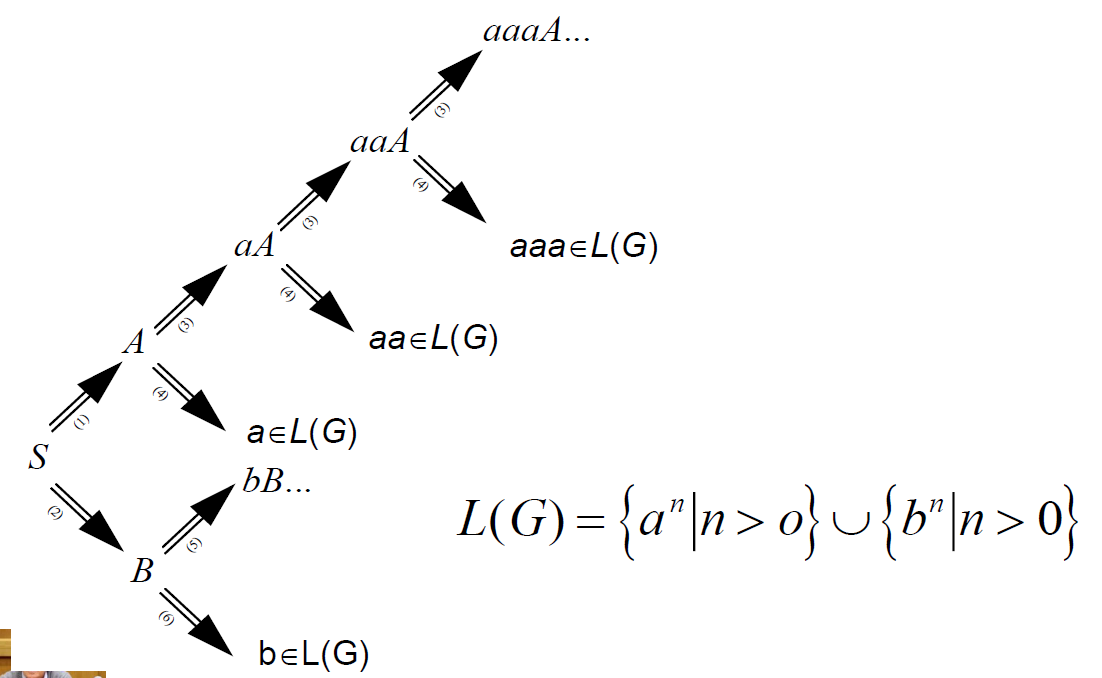
\includegraphics[width=1.00\textwidth]{generazione_linguaggio}
	\end{figure}
	Dunque, una grammatica è uno \textbf{strumento generativo} di un linguaggio perchè, data una qualsiasi parola di quel linguaggio, possiamo risalire mediante le produzioni al simbolo di partenza della grammatica. \\
	Viceversa, dato il simbolo di partenza di una grammatica, seguendo uno qualsiasi dei cammini dell'albero di derivazione, si produce una parola "valida" del linguaggio. \\
	In generale, dato un linguaggio $L$ ed una grammatica $G$, \textbf{non esiste un algoritmo} in grado di dimostrare che la grammatica genera il linguaggio, ossia che $L = L(G)$. \\
	Più specificatamente, non esiste un algoritmo che stabilisce se una data stringa è generata o no dalla grammatica presa in considerazione. \\
	Quindi:
	{
		\theorem{Il problema di dimostrare la correttezza di una grammatica non è risolubile algoritmicamente, in generale.}
	} \\
	In molti casi importanti, però, è possibile dimostrare per induzione che una particolare grammatica genera proprio un particolare linguaggio. \\
	Queste dimostrazioni ci consentono di stabilire se, data una grammatica $G$ ed un linguaggio $L$, risulta:
	\begin{itemize}
		\item $w \in L(G) \Rightarrow w \in L$ quindi $L(G) \subseteq L$ \\
		Ovvero, questo ci dice se la grammatica $G$ genera solo stringhe appartenenti al linguaggio $L$, quindi verifica la proprietà di \textbf{coerenza} o \textbf{consistenza} di $G$.
		\item $w \in L \Rightarrow w \in L(G)$ quindi $L \subseteq L(G)$ \\
		Ovvero, questo ci dice se il linguaggio $L$ comprende solo parole generabili dalla grammatica $G$, quindi verifica la proprietà di \textbf{completezza} di $G$.
	\end{itemize}
	Per dimostrare queste due proposizioni si utilizza il principio d'induzione che può essere di due forme:
	\begin{enumerate}
		\item Sia $n_0$ un intero e sia $P = P(n)$ un enunciato che ha senso per ogni intero $n \geq n_0$. Se:
		\begin{itemize}
			\item $P(n_0)$ è vero
			\item $\forall n > n_0, P(n-1)$ vero implica $P(n)$ vero
		\end{itemize}
		allora $P(n)$ vero per tutti gli $n \geq n_0$
		\item \textbf{Forma: Noetheriana} \\
		Sia $n_0$ un intero e sia $P=P(n)$ un enunciato che ha senso per ogni intero maggiore o uguale ad $n_0$. Se:
		\begin{itemize}
			\item $P(n_0)$ è vero;
			\item $\forall n, m \quad n>m\geq n_0$, $P(m)$ vero implica $P(n)$ vero
		\end{itemize}
		allora $P(n)$ vero per tutti gli $n \geq n_0$
	\end{enumerate}
	\chapter{Linguaggi liberi da contesto e linguaggi dipendenti da contesto}
	\section{Grammatica e linguaggi liberi da contesto} 
	{
		\definition[Grammatica libera da contesto]{Una grammatica $G = (X, V, S, P)$ è \textit{libera da contesto} o \textit{context-free, C.F} se, per ogni produzione, 
		\[
		v \to w
		\]
		$v$ è un nonterminale.
		}
		$G$ è libera da contesto $\overset{def}{\iff} \forall v \to w \in P \mid v \in V$
		\definition[Linguaggio libero da contesto]{Un linguaggio $L$ su un alfabeto $X$ è \textit{libero da contesto} se può essere generato da una grammatica libera da contesto \\
		$L$ libero da contesto $\overset{def}{\iff} \exists G$ libera da contesto tale che $L(G) = L$}
	}
	La maggior parte dei linguaggi di programmazione sono  C.F. Il termine C.F nasce dal fatto che la sostituzione di un \textit{NT} non è condizionata dal contesto ossia dai caratteri adiacenti in cui compare.  \\
	Un $NT\ A$ in una forma di frase può essere sempre sostituito usando una produzione del tipo $A \to \beta$ e la sostituzione risulta sempre valida. \\
	Viceversa, se $L = L(G)$ e $G$ \textbf{non} è C.F, \textbf{non} possiamo concludere che $L$ non è C.F perchè non possiamo escluder che esista una grammatica C.F $G'$ per cui $L = L(G')$.
	\textbf{Esempi di linguaggi C.F}:
	\begin{itemize}
		\item Il linguaggio delle parentesi ben formate;
		\item Il linguaggio dei numeri interi relativi;
		\item Il linguaggio $L = \{a^nb^n \mid n > 0\}$
		\item Il linguaggio delle stringhe con ugual numero di 0 e di 1.
		\item Il linguaggio $L = \{a^nb^{2n} \mid n > 0\}$
	\end{itemize}
	\section{Grammatiche e linguaggi dipendenti da contesto}
	{
		\definition[Grammatica dipendente da contesto]{Una grammatica $G = (X,V,S,P)$ è \textit{dipendente da contesto} o \textit{context-sensitive, C.S} se ogni produzione è in una delle seguenti forme:
		\begin{enumerate}
			\item $yAz \to ywz$ con $A \in V$, $y,z \in (X \cup V)^*$, $w \in (X \cup V)^+$ che si legge: $A$ può essere sostituita con $w$ nel contesto $y-z$, contesto sinistro $y$ e contesto destro $z$.
			\item $S \to \lambda$ purchè $S$ non compaia nella parte destra di alcuna produzione 
		\end{enumerate}
		}
		\definition[Linguaggio dipendente da contesto]{
			Un linguaggio $L$ è \textit{dipendente da contesto} se può essere generato da una grammatica dipendente da contesto. \\
			$L$ dipendete da contesto $\overset{def}{\iff}\exists G$ dipendente da contesto tale che $L(G) = L$
		}
	}
	\section{Relazione tra linguaggi C.F e C.S}
	\begin{figure}[H]
		\centering
		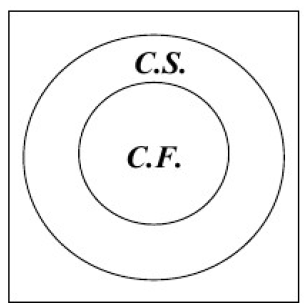
\includegraphics[width=0.75\textwidth]{relazione_CF_CS}
		\caption{Linguaggi formali}
	\end{figure}
	Tale relazione sussiste perchè le regole di produzione C.S sono una generalizzazione di quelle C.F. \\
	Le produzioni C.F sono un caso particolare delle produzioni di tipo $yAz \to ywz$ delle grammatiche C.S, che si verifica quando: $y=z=\lambda$ quindi quando contesto destro e sinistro sono equivalenti alla parola vuota, ma c'è un'eccezione. \\
	Osservando con attenzione la definizione di grammatica C.F si nota che, $w \in (X \cup V)^*$ mentre nella definizione di grammatica C.S, $w \in (X \cup V)^+$. \\
	Dunque le grammatiche C.F ammettono produzioni del tipo $A \to \lambda$ con $A$ che può anche non essere il simbolo iniziale, mentre le grammatiche C.S non ammettono tali produzioni. \\
	Queste tipologie di produzioni verranno chiamate \textit{\textbf{$\lambda-produzioni$} o \textit{\textbf{$\lambda-regole$}}} \\
	\textbf{Esempi di produzioni contestuali}:
	\begin{itemize}
		\item $bC \to bc$
		\item $baACbA \to baAabA$
	\end{itemize}
	\textbf{Esempio di grammatica contestuale:}
	\begin{itemize}
		\item $S \to \lambda | bC$
		\item $bC \to bc$
	\end{itemize}
	\textbf{Esempio di produzione non C.S né C.F}
	\begin{itemize}
		\item $CB \to BC$ \\
		Questa produzione non è né C.S né C.F. Questa si chiama produzione \textbf{monotona} perchè del tipo $v \to w$ con $|v| \leq |w|$
	\end{itemize}
	\section{Grammatiche e linguaggi monotoni}
	{
		\definition[Grammatica monotona]{
			Una grammatica $G=(X, V, S, P)$ è \textbf{monotona} se ogni sua produzione è monotona, cioè se
				\[
				\forall v \to w \in P \mid |v| \leq |w|
				\]
			}
		\definition[Linguaggio monotono]{
			Un linguaggio $L$ è \textbf{monotono} se può essere generato da una grammatica monotona. \\
			$L$ monotono $\overset{def}{\iff} \exists G$ monotona tale che $L(G) = L$
		}
	}
	\textbf{Esempio di produzioni monotone}:
	\begin{itemize}
		\item $AB \to CDEF$
		\item $CB \to BC$
	\end{itemize}
	Una produzione monotona può essere sostituita da una sequenza di produzioni contestuali senza alterare il linguaggio generato.
	Infatti $AB \to CDEF$ può essere sostituito dalle seguenti produzioni contestuali:
	\begin{itemize}
		\item $AB \to AG$
		\item $AG \to CG$ 
		\item $CG \to CDEF$
	\end{itemize}
	Oppure $CB \to BC$ può essere sostituita dalle seguenti produzioni contestuali:
	\begin{itemize}
		\item $CB \to XB$
		\item $XB \to XC$
		\item $XC \to BC$
	\end{itemize}
	oppure:
	\begin{itemize}
		\item $CB \to X_1B$
		\item $X_1B \to X_1X_2$
		\item $X_1X_2 \to X_1C$
		\item $X_1C \to BC$
	\end{itemize}
	{
	\theorem[Relazione linguaggi contestuali e monotoni]{
		La classe dei linguaggi contestuali coincide con la classe dei linguaggi monotoni:
		\begin{figure}[H]
			\centering
			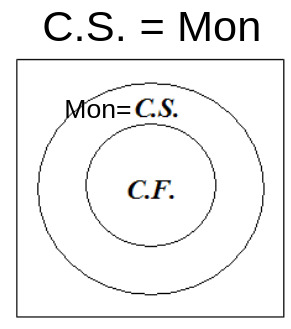
\includegraphics[width=0.75\textwidth]{linguaggi_monotoni_contestuali}
		\end{figure}
		Il teorema è il seguente: \\
		Sia $G$ una grammatica monotona, cioè tale che ogni produzione di $G$ è della forma $v \to w$ con $|v| \leq |w|$, eccetto che ci può essere un'unica $\lambda-produzione$: $S \to \lambda$ se $S$ non appare alla destra di una produzione. Esiste allora una grammatica C.S $G'$ equivalente a $G$, cioè tale che $L(G) = L(G')$. \\
		Tale teorema può essere enunciato anche nel seguente modo: \\
		Un linguaggio $L$ è dipendente da contesto se e solo se esiste una grammatica $G$ tale che $L = L(G)$ ed ogni produzione di $G$ nella forma $u \to v$ ha la proprietà che $0 < |u| \leq |v|$, con una sola eccezione: se $\lambda \in L(G)$ allora $S \to \lambda$ è una produzione di $G$ ed in tal caso $S$ non può comparire nella parte destra di altre produzioni. \\
		\proof{
			\begin{itemize}
				\item $\Rightarrow)$ Banale. \\
				Se $L$ è dipendente da contesto allora, per definizione, esiste $G$ dipendente da contesto tale che $L = L(G)$. \\
				$L$ è C.S $\overset{def}{\iff} \exists G$ C.S $\mid L = L(G)$. \\
				Allora ogni produzione di $G$ è in una delle due forme:
				\begin{enumerate}
					\item $yAz \to ywz$ con $A \in V$, $y,z \in (X \cup V)^*, w \in (X \cup V)^+$
					\item $S \to \lambda$ con $S$ che non compare nella parte destra di alcuna produzione.
				\end{enumerate}
				Dunque, ogni produzione di $G$ verifica la condizione $u \to v$ con $0< |u| \leq |v|$, se è del primo tipo, mentre se è del secondo tipo con $S$ che non compare a destra di alcuna produzione, ricade nell'eccezione. Pertanto $G$ è la grammatica cercata.
				\item $\Leftarrow)$ \\
				Sia $G$ una grammatica in cui ogni produzione è nella forma $u \to v$ con $0 < |u| \leq |v|$. Senza ledere la generalità della dimostrazione, possiamo supporre che una generica produzione di $G$ abbia il formato: 
				\[
				A_1A_2\dots A_m\to B_1B_2 \dots B_n \quad m \leq n
				\]
				Fare questa assunzione è legittimo in quanto, se $A_j$ fosse un terminale potremmo sostituirlo nella produzione con un nuovo nonterminale ed aggiungere la produzione $A_j' \to A_j$. \\
				Denotiamo con $C_1, C_2, \dots, C_m$ $m$ simboli non terminali non presenti in $G$ che rappresentano le nostre variabili di comodo. \\
				Utilizziamo le $C_k, k=1,2,\dots, m$ per costruire nuove regole contestuali che riscrivono la stringa $A_1A_2\dots A_m$ con $B_1B_2\dots B_n$. \\
				$A_1A_2\dots A_m \to C_1A_2 \dots A_m$ \\
				$C_1A_2 \dots A_m \to C_1C_2A_3 \dots A_,m$ \\
				\dots \\
				$C_1C_2\dots C_{m-1}A_m \to C_1C_2\dots C_{m-1}C_mB_{m+1}\dots B_n$ \\
				$C_1C_2 \dots C_{m-1}C_mB_{m+1}\dots B_n \to C_1\dots C_{m-1}B_mB_{m+1}\dots B_n$ \\
				\dots \\
				$C_1B_2\dots B_n \to B_1B_2\dots B_n$ \\
				La nuova grammatica che incorpora queste produzioni è contestuale e si può dimostrare che $L(G) = L(G')$
			\end{itemize}
		
		}
	}
	}
	\textbf{Esempio:} Sia $ABC \to DEFGH$
	\begin{enumerate}
		\item $ABC \to C_1BC$
		\item $C_1BC \to C_1C_2C$
		\item $C_1C_2C \to C_1C_2C_3GH$
		\item $C_1C_2C_3GH \to C_1C_2FGH$
		\item $C_1C_2FGH \to C_1EFGH$
		\item $C_1EFGH \to DEFGH$
	\end{enumerate}
	\chapter{Linguaggi liberi da contesto}
	\section{Alberi di derivazione}
	Le derivazioni di una grammatica libera da contesto possono essere rappresentate da \textit{alberi} detti \textbf{\textit{alberi di derivazione}}. \\
	La sequenza delle regole sintattiche utilizzate per generare una stringa $w$ da una grammatica $G$ di simbolo iniziale $S$ definisce la \textit{struttura} di $w$, che potrebbe essere rappresentata da una delle derivazioni $S \overset{*}{\Rightarrow} w$. Al fine di disporre di una rappresentazione univoca, si preferisce ricorrere agli alberi di derivazione. \\
	{
		\definition[Albero]{Un \textbf{\textit{albero}} è un grafo orientato, aciclico, connesso e avente al massimo un arco entrante in ciascun nodo. \\
		La definizione rigorosa di albero è la seguente:
		\begin{itemize}
			\item Un \textit{albero T} è un insieme finito, non vuoto di vertici, chiamati nodi, tali che:
			\begin{itemize}
				\item esiste un vertice speciale, detto \textit{radice} dell'albero;
				\item esiste una partizione $T_1, T_2, \dots, T_m$ con $m \geq 0$, degli altri vertici, tale che esista un ordinamento $T_1, T_2, \dots, T_m$ e ogni sottoinsieme di vertici $T_i$ con $1 \leq i \leq m$ sia a sua volta un albero
			\end{itemize} 
			
		\end{itemize}
		Questa definizione è di tipo ricorsivo, ma non è circolare in quanto ogni sottoalbero $T_i$ contiene meno vertici dell'albero $T$. \\
		$T_1, T_2, \dots, T_m$ sono detti \textit{sottoalberi} di $T$. I vertici privi di discendenti sono le \textit{foglie} dell'albero, gli altri sono i \textit{nodi interni}.
		\\
		La stringa dei simboli che etichettano le foglie di un albero \textit{T}, letti nell'ordine da sinistra a destra, prende il nome di \textbf{\textit{frontiera}} di $T$.
		}
		\definition[Partizione]{Gli insiemi, non vuoti, $T_1, T_2, \dots, T_m$ con $m \geq 0$ costituiscono una \textit{partizione} di un insieme, non vuoto, $T$ se:
		\begin{itemize}
			\item $T_1 \cap T_j = \emptyset$ per $i \neq j, i, j = 1,2,\dots, m$ 
			\item $\mathlarger{\bigcup_{i=1}^{m}}T_i = T$
		\end{itemize}
		}
		\definition[Albero di derivazione]{Sia $G = (X, V, S, P)$ una grammatica C.F e $w \in X^*$ una stringa derivabile da $S$ in $G$, $S \overset{*}{\Rightarrow} w$.	\\
		Dicesi \textbf{\textit{albero di derivazione}} per $w$ l'albero $T_w$ avente le seguenti proprietà:
		\begin{enumerate}
			\item la radice è etichettata con il simbolo iniziale $S$; 
			\item ogni nodo interno, nodo non foglia, è etichettato con un simbolo di $V$;
			\item ogni nodo foglia è etichettato con un simbolo di $X$ o con $\lambda$;
			\item se un nodo $N$ è etichettato con $A$, ed $N$ ha $k$ discendenti diretti $N_1, N_2, \dots, N_k$, etichettati con i simboli $A_1, A_2, \dots, A_k$ rispettivamente, allora la produzione:
			\[
			A \to A_1A_2\dots A_k
			\] 
			\begin{center}
				\begin{tikzpicture}
					% Nodo principale A
					\node (A) at (0,3) {$A$};
					
					% Nodi figli
					\node (A1) at (-2,0) {$A_1$};
					\node (A2) at (-0.5,0) {$A_2$};
					\node (Adots) at (1,0) {$\ldots$};
					\node (Ak) at (2.5,0) {$A_k$};
					
					% Linee di connessione
					\draw (A) -- (A1);
					\draw (A) -- (A2);
					\draw[dashed] (A) -- (Adots);
					\draw (A) -- (Ak);
				\end{tikzpicture}
			\end{center}
			deve appartenere a $P$;
			\item la stringa $w$ può essere ottenuta leggendo e concatenando le foglie dell'albero da sinistra a destra.
		\end{enumerate}
		}
		\definition[Lunghezza di un cammino]{
			Dato un albero di derivazione, la \textbf{\textit{lunghezza di un cammino}} dalla radice ad una foglia è data dal numero di nonterminali su quel cammino
		}
		\definition[Altezza o profondità]{
			L'\textbf{\textit{altezza}} di un albero è data dalla lunghezza del suo cammino più lungo.
		}
	} 
	Un albero di derivazione non impone alcun ordine sull'applicazione delle produzioni in una derivazione. In altri termini, \textit{data una derivazione, esiste uno ed un solo albero di derivazione} che la rappresenta, mentre \textit{un albero di derivazione rappresenta in generale più derivazi(oni}, in funzione dell'ordine col quale si espandono i non terminali.\\
	\textbf{Guardare esempio dalle slide}.
	\section{Principio di sostituzione di sottoalberi}
	{
		\definition[Derivazione destra (sinistra)]{Data una grammatica $G = (X, V, S, P)$, diremo che una derivazione $S \overset{*}{\Rightarrow} w$, ove:
		\[
		S \Rightarrow w_1 \Rightarrow w_2 \Rightarrow \dots \Rightarrow w_n = w
		\]
		\[
		w_i =y_iAz_i \quad w_{i+1}=y_iw_iz_i \quad i=1,2,\dots, n-1
		\]
		è destra (sinistra) se, per ogni $i, i=1,2,\dots, n-1$, risulta: 
		\[
		z_i \in X^*  \quad (y_i \in X^*)
		\]
		In altre parole in una \textbf{\textit{derivazione destra (sinistra)}} ad ogni passo si espande il nonterminale posto più a destra (sinistra).
		}
		
	} 
	\textbf{Esempio:} Riconsideriamo la grammatica che genera tutte e sole le stringhe che hanno un ugual numero di 1 e di 0. 
	\[
	S \to 0B|1A 
	\]
	\[
	A \to 0|0S|1AA
	\]
	\[
	B\to1|1S|0BB
	\]
	Consideriamo la stringa 0011. Una possibile derivazione è:
	\[
	S \Rightarrow 0B \Rightarrow 00BB \Rightarrow 001B \Rightarrow 0011
	\]
	Un'altra possibile è:
	\[
	S \Rightarrow 0B \Rightarrow 00BB \Rightarrow 00B1 \Rightarrow 0011
	\]
	Il non determinismo insito nella derivazione scompare quando si considera il relativo albero di derivazione. \\
	\begin{center}
		\begin{tikzpicture}[level distance=1.5cm, sibling distance=2cm]
			% Primo livello
			\node (S) {$S$}
			child {node (0a) {$0$}}
			child {node (B) {$B$}
				% Secondo livello sotto B
				child {node (0b) {$0$}}
				child {node (Ba) {$B$}
					% Terzo livello sotto il secondo B
					child {node (1a) {$1$}}
				}
				child {node (Bb) {$B$}
					% Terzo livello sotto il terzo B
					child {node (1b) {$1$}}
				}
			};
		\end{tikzpicture}
	\end{center}
	Consideriamo ora il sottoalbero con radice nel nodo con profondità minore etichettato con una $B$:
	\begin{figure}[H]
		\centering
		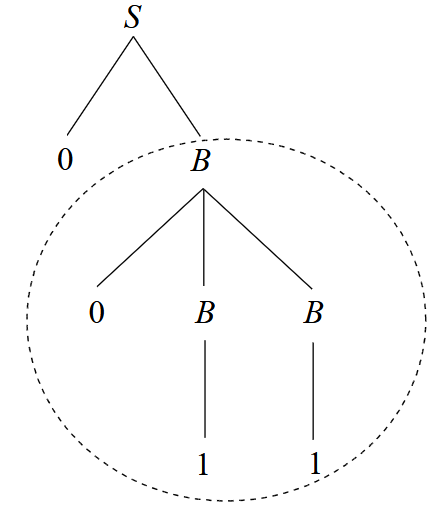
\includegraphics[width=0.50\textwidth]{sostituzione_alberi}
	\end{figure}
	Cosa accade se un qualsiasi sottoalbero con radice il nodo etichettato con una $B$ viene sostituito con il sottoalbero cerchiato nella figura precedente? \\
	Il nuovo albero è ancora un albero di derivazione e il nuovo albero di derivazione è rappresentato nella seguente figura:
	\begin{center}
		\begin{tikzpicture}[
			level 1/.style={sibling distance=4cm},
			level 2/.style={sibling distance=3cm},
			level 3/.style={sibling distance=2cm},
			level distance=1.8cm
			]
			% Primo livello
			\node (S) {$S$}
			child {node (0a) {$0$}}
			child {node (B1) {$B$}
				% Secondo livello sotto il primo B
				child {node (0b) {$0$}}
				child {node (B2) {$B$}
					% Terzo livello sotto il secondo B
					child {node (0c) {$0$}}
					child {node (B3) {$B$}
						% Quarto livello sotto il terzo B
						child {node (1a) {$1$}}
					}
					child {node (B4) {$B$}
						% Quarto livello sotto il quarto B
						child {node (1b) {$1$}}
					}
				}
				child {node (B5) {$B$}
					% Terzo livello sotto il quinto B
					child {node (1c) {$1$}}
				}
			};
		\end{tikzpicture}
		 \\
		per cui: $S \overset{*}{\Rightarrow} 000111$
	\end{center}
	Possiamo ripetere indefinitamente questo processo di sostituzione di sottoalberi, ottenendo parole del linguaggio di lunghezza crescente:
	\[
	\begin{array}{l}
		0011\phantom{0011} \quad |w|=4 \\
		000111\phantom{01} \quad |w|=6 \\
		00001111 \quad |w|=8 \\
		\dots \\
		00^n11^n \quad |w|=2n+2 \quad n=1,2,\dots
	\end{array}
	\]
	La lunghezza cresce in maniera costante. \\
	Nelle grammatiche C.F, dunque, possiamo sostituire alberi più piccoli con alberi di dimensioni maggiori, purchè abbiano la stessa radice, più precisamente, purchè i nodi radice siano etichettati con lo stesso $NT$, ottenendo ancora alberi di derivazione validi. \\
	Una caratteristica dei linguaggi C.F, che discende direttamente dal processo descritto in precedenza, è che la lunghezza delle parole cresce in maniera costante. \\
	Dunque, se una grammatica genera parole la cui lunghezza cresce in maniera esponenziale (o lineare o quadratica o cubica o ...) allora il linguaggio generato non è libero, vedi $L = {a^nb^nc^n | n > 0}$. \\
	Generalizziamo ora il discorso: supponiamo di avere un albero di derivazione $T_z$ per una stringa $z$ di terminali generata da una grammatica C.F $G$, e supponiamo inoltre che il simbolo $NT\ A$ compaia due volte su uno stesso cammino. La situazione è rappresentata graficamente in figura:
	\begin{figure}[H]
		\centering
		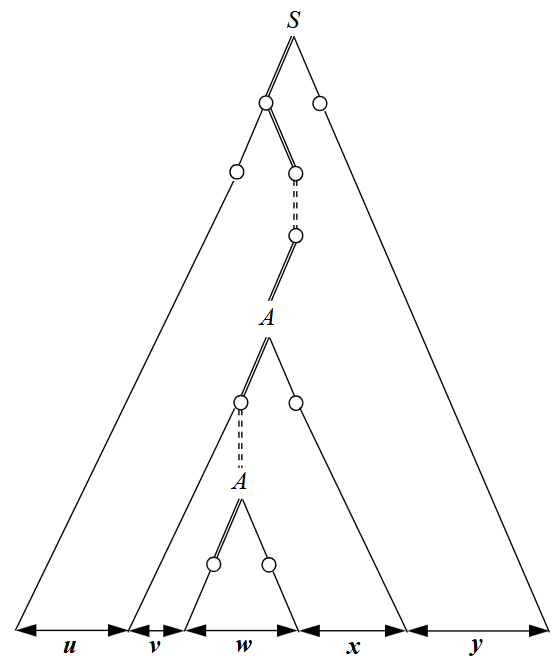
\includegraphics[width=0.75\textwidth]{teorema_sostituzione_alberi}
	\end{figure}
	Il sottoalbero più in basso con radice nel nodo etichettato con una $A$ genera la sottostringa $w$, mentre quello più in alto genera la sottostringa $vwx$. Poichè la $G$ è C.F., sostituendo il sottoalbero più in alto con quello più in basso si ottiene ancora una derivazione valida Il \textit{nuovo albero} genera la \textit{stringa} $uwy$. \\
	Se effetuiamo la sostituzione inversa, il sottoalbero più in basso viene rimpiazzatoda quello più in alto, otteniamo un albero di derivazione lecito per la stringa $uvvwxxy$ ossia $uv^2wx^2y$. Ripetendo questa sostituzione un numero finito di volte, si ottiene l'insieme di stringhe:
	\[
	\{uv^nwx^ny | n \geq 0\}
	\]
	{
		\proposition{Ogni linguaggio C.F infinito deve contenere almeno un sottoinsieme infinito di stringhe della forma:
		\[
		uv^nwx^ny \quad n \geq 0
		\]
		}
		\lemma{Sia $G = (X, V, S, P)$ una grammatica C.F e supponiamo che:
		\[
		m = max\{|v| \mid A \to v \in P\}
		\]
		Sia $T_w$ un albero di derivazione per una stringa $w$ di $L(G)$. Se l'altezza di $T_w$ è al più uguale ad un intero $j$, allora: $|w| \leq m^j$ \\
		In formule: $height(T_w) \leq j \Rightarrow |w| \leq m^j$
		Dove $m$ rappresenta la produzione più lunga e quindi l'ariabilità dell'albero e quindi notiamo che la lunghezza della stringa cresce in maniera esponenziale rispetto all'altezza dell'albero.
		\proof{La dimostrazione vale per un albero di derivazione che abbia come radice un qualunque simbolo $NT$, non necessariamente $S$. \\
		Procediamo per induzione su  $j$. 
		\begin{itemize}
			\item \textbf{Passo base: \quad $j=1$} \\
			$T_w$ rappresenta un'unica produzione, dunque la parola generata è composta al più da $m$ caratteri terminali e si ha: $|w| \leq m$
			\item \textbf{Passo induttivo:} \\
			Supponiamo che il lemma valga per ogni albero di altezza al più uguale a $j$ e la cui radice sia un simbolo $NT$ e dimostriamolo per un albero di altezza $j+1$. \\
			Supponiamo che il livello più alto dell'albero rappresenti la produzione $A \to v$, dove $v=v_1v_2\dots v_k$, $|v|=k$, $k \leq m$. \\
			Ogni simbolo $v_i, i=1,2,\dots,k$ di $v$ può essere radice di un sottoalbero di altezza al più uguale a $j$, poichè $T_w$ ha altezza uguale a $j+1$ (un $v_i$ potrebbe anche essere un terminale). \\
			Dunque, per ipotesi di induzione, ciascuno di questi alberi ha al più $m^j$ foglie. Poichè $|v|=k\leq m$, la stringa $w$, frontiera dell'albero $T_w$, ha lunghezza:
			\[
			|w| \leq m^j+m^j+\dots+m^j = |v|\cdot m^j=k\cdot m^j \leq m \cdot m^j = m^{j+1}
			\]
		\end{itemize}
		}
		}
	}
	\section{Pumping Lemma per i linguaggi liberi da contesto o teorema $uvwxy$}
	{
	\theorem[Pumping Lemma]{
		Sia $L$ un linguaggio libero da contesto. Allora esiste una costante $p$, che dipende solo da $L$, tale che se $z$ è una parola di $L$ di lunghezza maggiore di $p\ (|z| > p)$, allora $z$ può essere scritta come $uvwxy$ in modo tale che:
		\begin{enumerate}
			\item $|vwx| \leq p$
			\item al più uno tra $v$ e $x$ è la parola vuota $(vx \neq \lambda)$
			\item $\forall i, i \geq 0 \mid uv^iwx^iy \in L$
		\end{enumerate}
	}
	}
	Dato un linguaggio generato da una grammatica che non è C.F, non possiamo immediatamente escludere che non esiste una grammatica C.F che generi lo stesso linguaggio. Se un linguaggio infinito non rispecchia le proprietà del Pumping Lemma allora non può essere generato da una grammatica C.F. \\
	Il Pumping Lemma per i linguaggi liberi fornisce una \textbf{condizione necessaria} affinché un linguaggio sia libero.\[
	L\ \text{libero } \implies \exists p, \dots
	\]
	Dunque può essere utilizzato per dimostrare che un linguaggio non è libero con una dimostrazione per assurdo. \[
	\centernot{\exists}p, \dots \implies L\ \text{non è libero}
	\]
	{
	\proof[Pumping Lemma]{
		Sia $G = (X, V, S, P)$ una grammatica C.F che genera $L$. Denotiamo con $m$ il numero di simboli della più lunga parte destra di una produzione di $G$: \[
		m = max\{|v| \mid A \to v \in P\}
		\]
		Denotiamo con $k$ la cardinalità dell'alfabeto nonterminale di $G$:
		\[
		k = |V|
		\]
		Poniamo $p = m^{k + 1}$ e sia $z \in L$, con $|z| > p$\\
		Per il lemma precedente:
		\[
		[(height(T_z) \leq j \implies |z| \leq m^j)\ \iff (|z| > m^j \implies height(T_z) > j)]
		\]
		Se $|z| > p=m^{k + 1}$ allora ogni albero di derivazione per $z$ deve avere altezza maggiore di $k + 1$. \\
		Dunque, in ogni albero di derivazione per $z$ deve esistere almeno un cammino di lunghezza non inferiore a $k + 2$. \\
		Poichè $k=|V|$, almeno due $NT$ devono comparire duplicati su quel cammino o un $NT$ deve essere ripetuto 3 o più volte sul cammino. Senza ledere la generalità della dimostrazione, denotiamo con $A$ il $NT$ che compare duplicato per ultimo su quel cammino. Non vi sono pertanto altri $NT$ ripetuti almeno due volte al di sotto della $A$ più in alto. \\
		Questa considerazione implica che il cammino dalla $A$ più in alto della coppia ad una foglia ha lunghezza al più $k + 1$. \\
		Indichiamo con $vwx$ la sottostringa derivata dal sottoalbero avente radice nella $A$ più alta della coppia, ove $w$ è la sottostringa derivata dal sottoalbero avente radice nella $A$ più bassa della coppia. \\
		Dal Lemma, si ha:
		\[
		|vwx| \leq m^{k + 1} = p
		\]
		per cui risulta dimostrata la prima proprietà del Pumping Lemma. \\
		Scriviamo $z$ nella forma $uvwxy$, ed applichiamo il principio di sostituzione di sottoalberi. Se sostituiamo al sottoalbero avente radice nella $A$ più alta della coppia quello avente radice nella $A$ più bassa, otteniamo un albero di derivazione per la stringa:
		\[
		uwy=uv^0wx^0y
		\]
		che è la terza proprietà per $i = 0$. \\
		Se operiamo la sostituzione inversa, otteniamo un albero di derivazione per la stringa $uvvwxxy=uv^2wx^2y$ che è la terza proprietà per $i = 2$. \\
		Se ripetiamo la suddetta sostituzione $i-1$ volte, la stringa derivata è:$uv^iwx^iy$ per cui la terza proprietà risulta dimostrata. \\
		La seconda proprietà può essere dimostrata per assurdo. \\
		Sia $v=x=\lambda$. \\
		La sostituzione del sottoalbero avente radice nella $A$ più alta della coppia con quello avente radice nella $A$ più bassa della coppia non provoca alcun cambiamento nella stringa $z$ derivata dall'intero albero. Ma tale sostituzione provoca la diminuzione della lunghezza del cammino che dalla $A$ più in alto porta ad una foglia. Dunque, anche il cammino di lunghezza non inferiore a $k+2$ nell'albero di derivazione per $z$ risulta accorciato. In questo modo abbiamo ottenuto un albero di derivazione per $z$ con altezza almeno uguale a $k + 1$. Ma questo è assurdo per il Lemma.
	}
	}
\section{Grammatica ambigua}
{
\definition[Grammatica ambigua]{Una grammatica $G$ libera da contesto è \textbf{ambigua} se esiste una stringa $x$ in $L(G)$ che ha due alberi di derivazione differenti. \\
In modo alternativo, $G$ è ambigua se esiste una stringa $x \in L(G)$ che ha due derivazioni sinistre o destre distinte.}
}
La seguente grammatica libera da contesto:
\[
G_2 = (X, V, S, P)
\]
\[
X = \{a, +\} \quad V = \{S\} \quad P = \{S \to S + S, S \to a\}
\]
è ambigua. Infatti la stringa $w = a + a + a$ in $L(G_2)$ ha due differenti alberi di derivazione:
\begin{figure}[H]
	\centering
	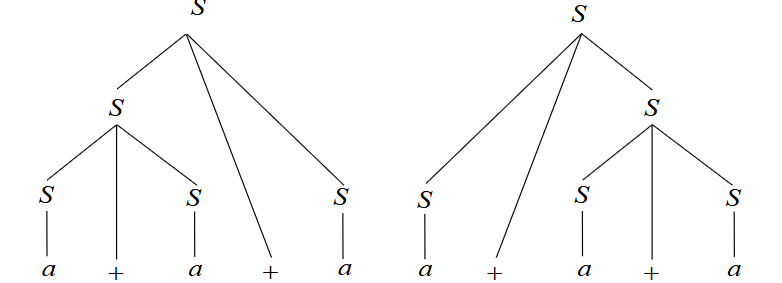
\includegraphics[width=1.00\textwidth]{grammatica_ambigua}
\end{figure}
Nel linguaggio naturale, l'ambiguità è un fenomeno intrinseco, che si verifica frequentemente. \\
Agli effetti delle applicazioni ai linguaggi di programmazione, l'ambiguità è una proprietà negativa. Infatti, il significato di una frase può essere definito come una funzione del suo albero di derivazione. \\
Inoltre, se esiste più di un albero di derivazione per una stessa frase, essa può avere un significato non univoco. Si preferisce quindi cercare una grammatica differente che, pur generando lo stesso linguaggio, non sia ambigua. L'unico vantaggio delle grammatiche ambigue, risulta essere il minore numero di regole che possono avere rispetto ad una grammatica non ambigua. \\
Ad esempio, il linguaggio precedente può essere generato anche dalla seguente grammatica:
\[
G_3 = (X, V, S, P)
\]
\[
X = \{a, +\} \quad V = \{S\} \quad P = \{S \to S + a, S \to a\}
\]
$G_3$ non è ambigua e inoltre: $L(G_2)=L(G_3)=\{aw \mid w \in \{+a\}^*\}$. \\
Esistono però dei linguaggi, detti \textbf{inerentemente ambigui}, per i quali tutte le grammatiche che li generano risultano ambigue. \\
\section{Linguaggio inerentemente ambiguo}
{
	\definition[Linguaggio inerentemente ambiguo]{Un linguaggio $L$ è \textit{\textbf{inerentemente ambiguo}} se ogni grammatica che lo genera è ambigua
	\[
	(\forall G)\ L = L(G):G\ \text{ambigua}
	\]
	}
}
Un linguaggio inerentemente ambiguo è: 
\[
L = \{a^ib^jc^k \mid (i = j \vee j = k)\}
\]
Intuitivamente, ci si rende conto di ciò pensando che in ogni grammatica che genera $L$ devono esistere due diversi insiemi di regole per produrre le stringe $a^ib^ic^k$ e le stringhe $a^ib^jc^j$. Le stringhe $a^ib^ic^i$ saranno necessariamente prodotte in due modi distinti, con distinti alberi di derivazione e conseguente ambiguità. \\
Vedere dal pdf altri esempi.
\chapter{Grammatiche e macchine}
\section{Classificazione delle grammatiche secondo Chomsky}
{
\definition[Gerarchia di Chomsky]{Sia $G = (X, V, S, P)$ una grammatica. Dalla definizione di grammatica, si ha:
\[
P = \{v \to w \mid v \in (X \cup V)^*V(X \cup V)^*, w \in (X \cup V)^*\}
\]
A seconda delle restrizioni imposte sulle regole di produzione, si distinguono le varie classi di grammatiche. 
\begin{itemize}
	\item \textbf{Tipo '0'}: Quando le stringhe che appaiono nella produzione $v \to w$ non sono soggette ad alcuna limitazione. 
	\item \textbf{Tipo '1' - Dipendente da contesto}: quando le produzioni sono limitate alla forma:
	\begin{enumerate}[(1)]
		\item $yAz \to ywz$ con $A \in V, \quad y,z \in (X \cup V)^*, \quad w \in (X \cup V)^+$
		\item $S \to \lambda$ purchè $S$ non compaia nella parte destra di alcune produzione.
 	\end{enumerate}
 	\item \textbf{Tipo '2' - Libera da contesto}: quando le produzioni sono limitate alla forma:
 	\[
 	v \to w \quad v \in V
 	\]
 	\item \textbf{Tipo '3' - Lineare destra}: quando le produzioni sono limitate alla forma:
   	\begin{enumerate}[(1)]
 		\item $A \to bC \quad A,C \in V \ e\ b \in X$
		\item $A \to b\phantom{C} \quad A \in V \ e\ b \in X \cup \{\lambda\}$
 	\end{enumerate}
\end{itemize}
}
}

Una grammatica di tipo '3' è detta \textit{lineare destra} perchè il $NT$, se c'è, compare nella parte destra della produzione. Un linguaggio generato da tale grammatica è detto di tipo '3' o \textit{lineare destro}. \\
\textbf{Esempi di linguaggi lineari destri}: \\
Consideriamo la grammatica $G_1$:
\[
S \to \lambda|0|0S|1|1S
\]
$G_1$ è lineare destra. $L(G_1) = {0, 1}^*$ ovvero l'insieme di tutte le stringhe binarie. \\
Consideriamo la grammatica $G_2$:
\[
S \to \lambda|0S|1T
\]
\[
T \to 0T|1S
\]
$G_2$ è lineare destra e $L(G_2) = \{w \in {0, 1}^* \mid w\ \text{ha un numero pari di 1}\}$
\subsection{Gerarchia dei linguaggi}
Dimostriamo formalmente che le quattro classi di linguaggi viste costituiscono una gerarchia. \\
\begin{figure}[H]
	\centering
	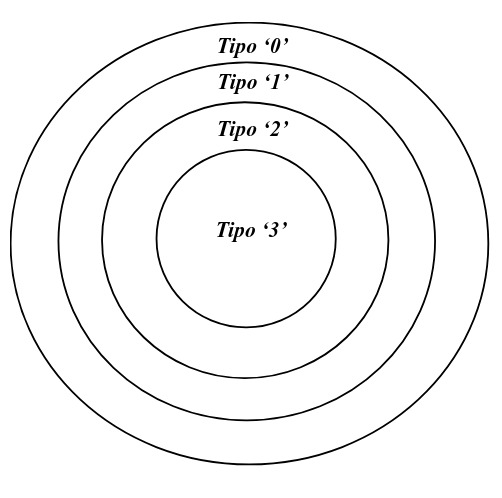
\includegraphics[width=.5\textwidth]{gerarchia_linguaggi}
\end{figure}
{
	\theorem[Teorema della gerarchia]{
		Denotiamo con \[
		\mathcal{L}_i = \{L \subset X^* \mid L = L(G), G\ \text{di tipo $i$}\}\]
		Ovvero la classe dei linguaggi di tipo $i$. \\
		La gerarchia di Chomsky è una gerarchia in senso stretto di classi di linguaggi:\[
			\mathcal{L}_3\underset{\neq}{\subset}\mathcal{L}_2 \underset{\neq}{\subset} \mathcal{L}_1 \underset{\neq}{\subset} \mathcal{L}_0
		\]
	}
	\proof[Teorema della gerarchia]{ \quad
	\begin{itemize}
		\item $\mathcal{L}_3 \underset{\neq}{\subset} \mathcal{L}_2$  \\
		Per dimostrare che la classe di linguaggi $\mathcal{L}_3$ è \textit{inclusa propriamente} nella classe di linguaggi $\mathcal{L}_2$ si deve dimostrare che ogni linguaggio di tipo '3' può essere generato da una grammatica di tipo '2' e che esiste almeno un linguaggio C.F di tipo '2'che non può essere generato da una grammatica di tipo '3'.
		\begin{itemize}
			\item $\mathcal{L}_3 \subseteq \mathcal{L}_2$ discende dalle definizioni di linguaggio di tipo '3' e di grammatica di tipo '2'. Infatti, si osserva facilmente che ogni grammatica di tipo '3' è anche una grammatica di tipo '2'.
			\item $\mathcal{L}_3 \neq \mathcal{L}_2$: posponiamo questa dimostrazione. \\
			Mostreremo che $L = \{a^kb^k \mid k > 0\}$ non è di tipo '3'.
		\end{itemize}
		\item $\mathcal{L}_2 \underset{\neq}{\subset} \mathcal{L}_1$ \\
		Abbiamo già osservato che le produzioni C.F sono un caso particolare delle produzioni C.S con l'unica eccezione rappresentata dalle produzioni:
		\[
		A \to \lambda \quad A \neq S
		\]
		che sono C.F ma \textbf{non} C.S. Dunque:
		\[
		\forall L: L \in \mathcal{L}_2 \overset{def}{\iff} \exists G, \text{G è C.F} : L = L(G)
		\]
		Se $A \to \lambda, A \in V \backslash \{S\}$ non è una produzione di G, allora G è anche C.S e l'asserto è dimostrato. Il problema sorge se G ha almeno una $\lambda$-produzione. In tal caso, ci avvaliamo del seguente risultato:
		\lemma[Stringa vuota]{
		Sia $G = (X, V, S, P)$ una grammatica C.F con almeno una $\lambda$-produzione. Allora esiste una grammatica C.F G' tale che:
		\begin{enumerate}[i)]
			\item $L(G)=L(G')$ 
			\item se $\lambda \notin L(G)$ allora in $G'$ non esistono produzioni del tipo $A \to \lambda$
			\item se $\lambda \in L(G)$ allora in $G'$ esiste un'unica produzione $S' \to \lambda$, ove $S'$ è il simbolo iniziale di $G'$ ed $S'$ non compare nella parte destra di alcuna produzione di $G'$.
		\end{enumerate}
		}
		Riprendiamo al dimostrazione di $\mathcal{L}_2 \underset{\neq}{\subset}\mathcal{L}_1$
		\[
		\forall L: L \in \mathcal{L}_2 \overset{def}{\iff} \exists G, \text{G è C.F} : L = L(G)
		\]
		Se G ha almeno una $\lambda$-produzione, utilizziamo il Lemma della stringa vuota per determinare una grammatica C.F G' equivalente a G, ma priva di $\lambda$-produzioni, al più, in G' compare la produzione $S'\to \lambda$, ed $S'$ non compare nella parte destra di alcuna produzione di $G'$ e allora $G'$ è di tipo '1'. \\
		Questo dimostra che $\mathcal{L}_2 \subseteq \mathcal{L}_1$. \\
		Per dimostrare $\mathcal{L}_2 \neq \mathcal{L}_1$ ci avvaliamo del linguaggio:
		\[
		L = \{a^nb^nc^n \mid n > 0\}
		\]
		che è di tipo '1' ma non di tipo '2'. Si osservi che, per asserire che $L$ è di tipo '1', ci siamo avvalsi del teorema che stabilisce l'equivalenza delle classi di linguaggi contestuali e monotoni. 
		\item $\mathcal{L}_1 \underset{\neq}{\subset}\mathcal{L}_0$ \\
		Non lo dimostriamo formalmente. La dimostrazione comporta la conoscenza delgi automi limitati lineari e delle macchine di Turing che riconoscono linguaggi di tipo '0' o ricorsivamente enumerabili. Ci limitiamo ad osservare che $\mathcal{L}_1 \subseteq \mathcal{L}_0$ discende direttamente dalle definizioni di linguaggi di tipo '1' e di grammatica di tipo '0'.
	\end{itemize}
	}
}
\section{Operazioni sui linguaggi}
Siano $L_1$ ed $L_2$ due linguaggi definiti su uno stesso alfabeto $X\ (L_1, L_2 \subseteq X^*)$. 
\begin{itemize}
	\item L'\textit{\textbf{unione}} di $L_1$ ed $L_2$ è:
	\[
	L_1 \cup L_2 = \{w \mid w \in L_1 \vee w \in L_2 \}
	\]
	\item La \textit{\textbf{concatenazione}} di $L_1$ ed $L_2$ anche detta \textit{il prodotto di $L_1$ ed $L_2$ o $L_1$ punto $L_2$} è:
	\[
	L_1 \cdot L_2 = \{w \mid w_1w_2, \quad w_1 \in L_1, \quad w_2 \in L_2\}
	\]
	\item L'\textit{\textbf{iterazione}} di $L_1$ o \textit{chiusura riflessiva transitiva} di $L_1$ rispetto all'operazione di concatenazione, anche detta \textit{stellatura di $L_1$} o \textit{$L_1$ star} o \textit{chiusura di Kleene} è: 
	\[
	L_1^* = \{w \mid w = w_1w_2\dots w_n, \quad n \geq 0 \ e\ \forall i: w_i \in L_1\}
	\]
	\item Il \textit{\textbf{complemento}} di $L_1$ è:
	\[
	\overline{L_1} = X^* - L_1
	\]
	\item L'\textit{\textbf{intersezione}} di $L_1$ e $L_2$ è:
	\[
	L_1 \cap L_2 = \{w \mid w \in L_1 \wedge w \in L_2\}
	\]
\end{itemize}
\subsection{Proprietà dei linguaggi}
Dati $L_1, L_2, L_3 \subseteq X^* \quad (\equiv L_1, L_2, L_3 \in 2^{X^*})$, risulta:
\begin{itemize}
	\item $(L_1 \cdot L_2) \cdot L_3 = L_1 \cdot (L_2 \cdot L_3)$
	\item $L_1 \cdot L_2 \neq L_2 \cdot L_1$
	\item $L_1 \cdot \{\lambda\} = \{\lambda\} \cdot L_1 = L_1$
\end{itemize}
$\{\lambda\}$ è l'elemento neutro rispetto all'operazione di concatenazione di linguaggi. \\
Dunque anche $(2^{X^*}, \cdot)$ è un monoide:
\begin{itemize}
	\item $L_1 \cdot \emptyset = \emptyset \cdot L_1 = \emptyset$ \quad $\emptyset$ è l'elemento assorbente
	\item Se $\lambda \in L_1 \quad$ \begin{align*}
		L_2 \subseteq L_1 \cdot L_2 \\
		L_2 \subseteq L_2 \cdot L_1
	\end{align*}
	\item Se $\lambda \in L_2 \quad $ \begin{align*}
		L_1 \subseteq L_1 \cdot L_2 \\
		L_1 \subseteq L_2 \cdot L_1
	\end{align*}
	\end{itemize}
	\section{Potenza di un linguaggio}
	{
		\definition[Potenza di un linguaggio]{Sia $L$ un linguaggio definito su un alfabeto $X$. Dicesi \textbf{\textit{potenza n-esima}} di $L$, e si denota con $L^n$, $n \geq 0$, il seguente linguaggio:
		\[
		L^n = \begin{cases}
			\{\lambda\} \quad \quad n = 0 \\
			L^{n-1}L \quad n \neq 0
		\end{cases}
		\]
		Posto:
		\[
		L^+ = \bigcup_{i \geq 1}L^i
		\]
		si ha:
		\[
		L^* = \{\lambda\} \cup L^+ = L^0 \cup L^+ = \bigcup_{i \geq 0}L^i
		\]
		}
	}
	$L^+$ è detta chiusura transitiva rispetto alla operazione di concatenazione. \\
	Dunque si ha:
	
	\[	L^0 = \{\lambda\} \]
	\[	L^1 = L^0 \cdot L = L \]
	\[	L^2 = L^1 \cdot L = (L^0 \cdot L)\cdot L \]
	\[	L^3 = L^2 \cdot L = (L^1 \cdot L) \cdot L = ((L^0 \cdot L) \cdot L) \cdot L \]
	Quindi, sia $L$ un linguaggio definito su un alfabeto $X$. Si ha:
	\[
	L^* = \bigcup_{i \geq 0}L^i = \{\lambda\} \cup L \cup L^2 \cup L^3 \cup \dots
	\]
	\section{Proprietà di chiusa delle classi di linguaggi}
	{
		\subsection{Teoremi di chiusura su unione, concatenazione e iterazione}
		\definition[Linguaggi definito su $X$]{
		$L$ è un \textit{\textbf{linguaggio}} definito su $X \overset{def}{\iff} L \subseteq X^* \iff L \in 2^{X^*}$ 
		}
		\definition[Classe di linguaggi]{$\mathcal{L}$ è una \textit{\textbf{classe di linguaggi}} su $X \overset{def}{\iff} \mathcal{L} \subseteq 2^{X^*} \iff \mathcal{L} \in 2^{2^{X^*}}$
		}
		\definition[Chiusura]{Sia $\mathcal{L}$ una classe di linguaggi su $X$. \\
		Sia $\alpha$ un'operazione binaria sui linguaggi di $\mathcal{L}$: 
		\[
		\alpha: 2^{X^*} \times 2^{X^*} \to 2^{X^*}, \quad (L_1, L_2) \mapsto \alpha(L_1, L_2)
		\]
		Sia $\beta$ un'operazione unaria sui linguaggi di $\mathcal{L}$:
		\[
		\beta: 2^{X^*} \to 2^{X^*}, \quad L \mapsto \beta(L)
		\]
		}
		$\mathcal{L}$ è \textbf{chiusa} rispetto ad $\alpha \overset{def}{\iff} \forall L_1, L_2 \in \mathcal{L} : \alpha(L_1, L_2) \in \mathcal{L}$ \\
		$\mathcal{L}$ è \textbf{chiusa} rispetto ad $\beta \overset{def}{\iff} \forall L_1 \in \mathcal{L} : \beta(L_1) \in \mathcal{L}$
		\theorem[Teorema di chiusura]{
		La classe dei linguaggi di tipo $i, i=0,1,2,3$ è chiusa rispetto alle operazioni di \textit{unione, concatenazione} ed \textit{iterazione}.\\
		\proof{La dimostrazione di questo teorema è \textit{\textbf{costruttiva}}. \\
		Siano $L_1$ ed $L_2$ due linguaggi:
		\[
		L_1 = L(G_1) \quad G_1 = (X, V_1, S_1, P_1)
		\]
		\[
		L_2 = L(G_2) \quad G_2 = (X, V_2, S_2, P_2)
		\]
		Assumiamo che $V_1 \cap V_2 = \emptyset \quad S \notin V_1 \cup V_2$ e nel caso in cui questa assunzione non sia vera, rinominiamo i nonterminali in comune. \\
		Poniamo:
		\[
		V = V_1 \cup V_2 \cup \{S\}
		\] 
		Lo schema generale della dimostrazione è il seguente:
		\begin{itemize}
			\item consideriamo un'operazione alla volta, denotata con $\alpha$;
			\item date $G_1$ e $G_2$, costruiamo $G$;
			\item si dimostra che, se $G_1$ e $G_2$ sono di tipo $i$, allora $G$ è di tipo $i$;
			\item si dimostra che $L(G) = \alpha(L_1, L_2)$ e dunque la classe di linguaggi $\mathcal{L}_i$ è chiusa rispetto alla operazione di $\alpha$.
		\end{itemize}
		\begin{enumerate}
			\item \textbf{Unione}: \\
			Costruiamo la grammatica: $G_3 = (X, V, S, P_3)$ ove:
			\[
			P_3 = \{S \to S_1, S \to S_2\} \cup P_1 \cup P_2
			\] 
			Osserviamo che, se $G_1$ e $G_2$ sono entrambe di tipo $i, i = 0, 1, 2$ lo è anche $G_3$. In ciascuno di questi casi, si ha:
			\[
			L(G_3) = L_1 \cup L_2
			\]
			Infatti una derivazione da $S$ in $G_3$ deve necessariamente iniziare o con:
			\begin{itemize}
				\item $S \Rightarrow S_1$ ed in tal caso può generare unicamente parole di $L(G_1)$
				\item $S \Rightarrow S_2$ ed in tal caso genera una parola di $L(G_2)$
			\end{itemize}
			Dunque, risulta dimostrato che $\mathcal{L}_0, \mathcal{L}_1, \mathcal{L}_2$ sono chiuse rispetto all'unione. \\
			Però, se $G_1$ e $G_2$ sono di tipo '3', $G_3$ non è lineare destra, perchè le produzioni $S \to S_1$ ed $S \to S_2$ non sono ammesse. \\
			Per avere ancora produzioni lineari destre che simulino il passo iniziale di una derivazione in $G_1$ ed anche il passo iniziale di una derivazione in $G_2$, costruiamo la grammatica $G_4 = (X, V, S, P_4)$ ove:
			\[
			P_4 = \{S \to w \mid S_1 \to w \in P_1\} \cup \{S \to w \mid S_2 \to w \in P_2\} \cup P_1 \cup P_2
			\]
			$G_4$ è lineare destra se $G_1$ e $G_2$ lo sono e inoltre:
			\[
			L(G_4) = L_1 \cup L_2 
			\]
			ed $\mathcal{L}_3$ è chiusa rispetto all'unione.
			\item \textbf{Concatenazione}: \\
			Costruiamo la grammatica: $G_5 = (X, V, S, P_5)$ ove:
			\[
			P_5 = \{S \to S_1S_2\} \cup P_1 \cup P_2
			\]
			Osserviamo che, se $G_1$ e $G_2$ sono entrambe di tipo $i, i = 0, 1, 2$ lo è anche $G_5$. \\
			Se $G_1$ e $G_2$ sono C.F, cioè di tipo '2', allora si ha:
			\[
			L(G_5) = L_1 \cdot L_2
			\]
			in quanto ogni derivazione da $S$ in $G_5$ ha la seguente "struttura":
			\[
			S \Rightarrow S_1S_2 \underset{G_1}{\overset{*}{\Rightarrow}} w_1S_2 \underset{G_1}{\overset{*}{\Rightarrow}} w_1w_2
			\]
			ove, evidentemente, si ha:
			\[
			S_1 \overset{*}{\Rightarrow} w_1 \quad S_2 \overset{*}{\Rightarrow} w_2
			\]
			Il seguente controesempio mostra che la condizione che $G_1$ e $G_2$ siano di tipo '2' è fondamentale per la validità di:
			\[
			L(G_5) = L_1\cdot L_2
			\]
			\textbf{Controesempio:} Consideriamo $G_1$ con $P_1 = \{S \to b\}$ e $G_2$ con $P_2 = \{bS_2 \to bb\}$. Da cui $L_1 = L(G_1) = \{b\}$ ed $L_2 = L(G_2) = \emptyset$. \\
			Dunque $L_1 \cdot L_2 = \emptyset$. \\
			Se costruiamo $G_5$ si ha: $P_5 = \{ S \to S_1S_2, S_1 \to b, S_2 \to bS_2\}$ ed $L(G_5) \neq \emptyset$ in quanto $S \overset{*}{\underset{G_5}{\Rightarrow}} bb$ attraverso la seguente derivazione: 
			\[
			S \Rightarrow S_1S_2 \Rightarrow bS_2 \Rightarrow bb
			\]
			Dunque la $G_5$ va bene solo per le grammatiche di tipo '2' e risulta dimostrato che $\mathcal{L}_2$ è chiusa rispetto alla concatenazione. \\
			La dimostrazione fatta non va bene per le grammatiche di tipo '0' e di tipo '1', in quanto entrambe queste classi di grammatiche presentano produzioni dipendenti da contesto. \\
			In presenza di grammatiche di tali tipo è necessario impedire che le derivazioni da $S_2$ si servano di precedenti derivazioni da $S_1$ e/o viceversa. In altri termini, è necessario evitare \textbf{interferenza tra derivazioni} da $S_1$ e derivazione da $S_2$ nella definizione dei contesti. È possibile ottenere ciò considerando copie distinte di $X$ in derivazioni distinte, in modo che nessun $NT$ derivato da $S_1$ possa far uso di parte di una forma di frase derivata da $S_2$ come contesto per l'applicazione di una produzione e viceversa. \\
			Siano pertanto:
			\[
			X'=\{x' \mid x \in X\} \quad X'' = \{x'' \mid x \in X\}
			\]
			due copie distinte di $X$ tali che:
			\[
			X' \cap X'' = \emptyset \quad X' \cap X = \emptyset \quad X' \cap V = \emptyset \quad X'' \cap X = \emptyset \quad X''\cap V = \emptyset
			\]
			e sia $P_1'$ l'insieme delle produzioni ottenute da $P_1$ sostituendo ogni occorrenza di un terminale $x$ in $X$ con il corrispondente nonterminale $x'\in X': P_1' = P_1\Big[\sfrac{x'}{x} \Big]$. \\
			Similmente, sia $P_2''$ l'insieme delle produzione ottenute da $P_2$ sostituendo ogni occorrenza di un terminale $x$ in $X$ con il corrispondente $x''$ in $X'': P_2'' = \Big[\sfrac{x''}{x}\Big]$. \\
			Costruiamo la grammatica: $G_6 = (X, V \cup X'\cup X'', S, P_6)$ ove:
			\[
			P_6 \{S \to S_1S_2\} \cup P_1'\cup P_2'' \cup \{x'\to x \mid x \in X\} \cup \{x'' \to x \mid x \in X\}
			\]
			Se $G_1$ e $G_2$ sono entrambe di tipo $i, i=0,1$ lo è anche $G_6$. \\
			Inoltre, si ha: $L(G_6) = L_1 \cdot L_2$. \\
			Il controesempio visto prima non dà più problemi:
			\[
			P_1' = \{S_1 \to b' \} \quad P_2'' = \{b''S_2 \to b''b''\}
			\]
			e:
			\[
			G_6 = (X, V \cup \{b'\} \cup \{b'' \}, S, P_6)
			\]
			dove:
			\[
			P_6 = \{S \to S_1S_2, S_1 \to b', b''S_2 \to b''b'', b' \to b, b'' \to b\}
			\]
			Risulta così dimostrato che $\mathcal{L}_0$ e $\mathcal{L}_1$ sono chiuse rispetto alla concatenazione. \\
			È immediato osservare che, se $G_1$ e $G_2$ sono di tipo '3' nè $G_5$ nè $G_6$ sono di tipo '3', per la produzione $S \to S_1S_2$. \\
			Osserviamo che, data una grammatica di tipo '3', ogni forma di frase derivata dal simbolo iniziale di tale grammatica ha due peculiarità:
			\begin{enumerate}[(1)]
				\item in essa compare al più un NT
				\item se in essa compare un NT, questo è il simbolo più a destra
			\end{enumerate}
			Modifichiamo pertanto ogni produzione del tipo $A \to b$ in $G_1$ in modo che essa non costituisca l'ultima produzione applicata in una derivazione da $S_1$ in $G_1$, ma possa innescare una derivazione da $S_2$ in $G_2$. Poniamo dunque a destra della $b$ il simbolo iniziale $S_2$ in $G_2$. \\
			Le produzioni del tipo $A \to b$ in $G_1$ vengono trasformate in: $A \to bS_2$. Costruiamo dunque la grammatica:
			\[
			G_7 = (X, V - \{S\}, S_1, P_7)
			\]
			ove:
			\[P_7 = \{A \to bB \mid A \to bB \in P_1\} \cup \{A\to bS_2 \mid A \to b \in  P_1, b \neq \lambda\} \cup \]
			\[\ \cup\ \{ A \to bS_2 \mid A \to bB \in  P_1, B \to \lambda \in P\}\]
			\[\phantom{P_7 =} \cup \{ S_1 \to w \mid S_2 \to w \in P_2, S_1 \to \lambda\in P_1\} \cup P_2\]
			La terzultima e penultima produzione sono state inserite per garantire la correttezza della grammatica generata, anche in presenza di $\lambda$-produzioni in $G_1$. \\
			$G_7$ è di tipo '3' se $G_1$ e $G_2$ lo sono ed inoltre:
			\[
			L(G_7) = L_1 \cdot L_2
			\]
			ed $\mathcal{L}_3$ è chiusa rispetto alla concatenazione. 
 			\item \textbf{Iterazione}: \\
 			Costruiamo la grammatica $G_8 = (X, V_1 \cup \{S\}, S, P_8)$ ove:
 			\[
 			P_8 = \{S \to \lambda, S \to S_1S\} \cup P_1
 			\]
 			Data la grammatica $G_1=\{X, V_1, S_1, P_1\}$ che genera $L_1$. la grammatica $G_8$ genera la parola vuota $\lambda$ e tutte le parole che si possono ottenere per concatenazione di parole generate da $S_1$ in $G_1$. Si ha infatti:
 			\[
 			S \overset{n}{\underset{G_8}{\Rightarrow}}S_1S_1\dots S_1S \Rightarrow S_1S_1\dots S_1 \overset{*}{\Rightarrow} w_1w_2\dots w_n
 			\]
 			con $w_i \in L_1, i = 1, 2, \dots, n$. \\
 			Vediamo per quali classi di grammatiche la $G_8$ è la grammatica che stiamo cercando:
 			\begin{itemize}
 				\item se $G_1$ è di tipo '3', $G_8$ non è di tipo '3', perchè non è lineare destra;
 				\item se $G_1$ è di tipo '2', $G_8$ è di tipo '2' e si ha: $:L(G_8) = L_1^*$;
 				\item se $G_1$ è di tipo '1', $G_8$ non è di tipo 1, perchè $S$ compare nella parte destra della produzione $S \to S_1S$ ed $S \to \lambda$ è una produzione in $P_8$: possiamo trasformare facilmente $G_8$ nella grammatica equivalente a $G_8'$, definita come segue:
 				\[
 				G_8'= \{X, V_1 \cup {S, S'}, S,P_8'\}
 				\]
 				\[
 				P_8' = \{S \to \lambda | S', S'\to S_1 | S_1S'\} \cup P_1
 				\]
 				ma $G_8'$ incorre nello stesso problema di interferenza nella definizione dei contesti visto per la concatenazione.
 				\item se $G_1$ è di tipo '0', lo è anche $G_8$, ma si incorre nello stesso problema di interferenza nella definizione dei contesti visto nella dimostrazione per la concatenazione.
 			\end{itemize}
 			Il problema dell'interferenza dei contesti, comune agli ultimi due casi $G_1$ di tipo $i, i=0,1$ esiste ancora come mostrato nel seguente controesempio: \\
 			\textbf{Controesempio:} Consideriamo $G_1$ con $P_1 = \{S_1 \to b, bS_1 \to bc\}$ allora $L_1 = L(G) = \{b\}$ e $L_1^* = \{b\}^*$. \\
 			Quindi:
 			\[
 			P_8 = \{S \to \lambda|S', S'\to S_1|S_1S', S_1 \to b, bS_1 \to bc\}
 			\]
 			Se consideriamo la derivazione:
 			\[
 			S \Rightarrow S'\Rightarrow S_1S' \Rightarrow S_1S_1 \Rightarrow bS_1 \Rightarrow bc
 			\]
 			si ottiene che $bc \in L(G_8')$ e quindi $L(G_8') \neq L_1^*$. \\
 			Il problema dell'interferenza dei contesti può essere risolto nel seguente modo. Eliminiamo le produzioni del tipo $S_1 \to \lambda$ e utilizziamo gli insiemi ausiliari $X'$ e $X''$ di $NT$ per evitare interferenze:
 			\[
 			X' = \{x' | x \in X\} \quad X''=\{x'' \mid x \in X\}
 			\]
 			\[
 			X'\cap X'' = \emptyset \quad X'\cap X = \emptyset \quad X' \cap V_1 = \emptyset
 			\]
 			\[
 			X'' \cap X = \emptyset \quad X'' \cap V_1 = \emptyset
 			\]
 			Consideriamo due copie di $G_1$:
 			\[
 			G_1'=\{X, V_1 \cup X', S_1, P_1'\}
 			\]
 			\[
 			G_1''=\{X, V_1 \cup X'', S_2, P_1''\}
 			\]
 			ove:
 			\[ P_1' = P_1\Big[\sfrac{x'}{x} \Big] \quad  P_1''= P_1\Big[\sfrac{x''}{x} \Big]\] 
 			Infine, combiniamo $G_1'$ e $G_1''$ con produzioni che costruiscono sequenze finite di copie di $S_1$ ed $S_2$ che si alternano, in modo da ottenere $L_1^*$. \\
 			Dunque, al grammatica che otteniamo è:
 			\[
 			G_9 = \{X, V_1 \cup X' \cup X'' \cup \{S,S_1, S_1', S_2, S'\}, S, P_9\}
 			\]
 			ove:
 			\[
 			P_9 = \{S \to \lambda|S_1'|S_2', S_1 \to S_1 | S_1S_2', S_2' \to S_2|S_2S_1'\} 
 			\]
 			\[
 			\phantom{P_9 =\ }
 			\cup P_1' \cup P_1'' \cup \{x' \to x\mid x\in X\} \cup \{x'' \to x \mid x\in X\}
 			\]
 			se $G_1$ è di tipo $i, i = 0,1$ lo è anche $G_9$ e si ha $L(G_9) = L_1^*$ e risulta dimostrato che $\mathcal{L}_0$ e $\mathcal{L}_1$ sono chiuse rispetto all'iterazione. \\
 			Resta da dimostrare che $L_3$ è chiusa rispetto all'iterazione. Per costruire la nuova grammatica, introduciamo dapprima un nuovo simbolo iniziale $S$ e la produzione $S \to \lambda$ che genera la stringa vuota. \\
 			Inoltre, eliminiamo da $P_1$, se c'era, la produzione $S_1 \to \lambda$ ed aggiungiamo una produzione $S \to w$ per ogni produzione iniziale $S_1 \to w$ in $P_1$. \\
 			Infine, per ogni produzione la cui parte destra contiene solo un terminale, del tipo $A \to b$, nell'insieme delle produzioni che stiamo costruendo, aggiungiamo la produzione $A \to bS$ in modo che, avendo derivata una forma di frase del tipo $w_1w_2\dots w_j'A$ tale che ogni sottostringa $w_1, w_2, \dots, w_j = w_j'b$ è una parola di $L_1$, abbiamo la possibilità di terminare la derivazione con $w_1w_2\dots w_j$ o di continuarla generando la forma di frase $w_1w_2 \dots w_jS$ che consente di generare una parola più lunga di $L_1^*$. \\
 			Si noti che, per garantire la correttezza della grammatica generata anche in presenta di $\lambda-$produzioni in $G_1$, occorre aggiungere una produzione $A \to bS$ per ogni produzione $A \to bB$ nell'insieme delle produzioni che stiamo costruendo, quando $B \to \lambda$ è una pura una produzione di tale insieme, alla stregua di quando fatto per la concatenazione in $\mathcal{L}_3$. \\
 			Costruiamo dunque la grammatica: $G_{10} = \{X, V_1 \cup \{S\}, S, P_10\}$, ove:
 			\[
 			P_{10} = \{S \to \lambda\} \cup (P_1 - \{S_1 \to \lambda\}) \cup \{S \to w \mid S_1 \to w \in P_1\} \cup
 			\]
 			\[
 			\phantom{P_{10} =\ }
 			\cup \{A \to bS \mid A \to b \in P_{10}, b \neq \lambda\} \cup
 			\]
 			\[
 			\phantom{P_{10} =\ }
 			\cup \{A \to bS \mid A \to bB \in P_{10} , B\to \lambda \in P_{10}\}
 			\]
 			Se $G_1$è di tipo '3', lo è anche $G_{10}$ e si ha: $L(G_{10}) = L_1^*$ e risulta dimostrato che $\mathcal{L}_3$ è chiusa rispetto all'iterazione.
		\end{enumerate}
		}
		}
	}
	Riassumiamo le modalità di costruzione che generano i linguaggi \textit{unione, concatenazione, iterazione} di $L_1$ ed $L_2$ nella tavola che segue:
	\begin{figure}[H]
		\centering
		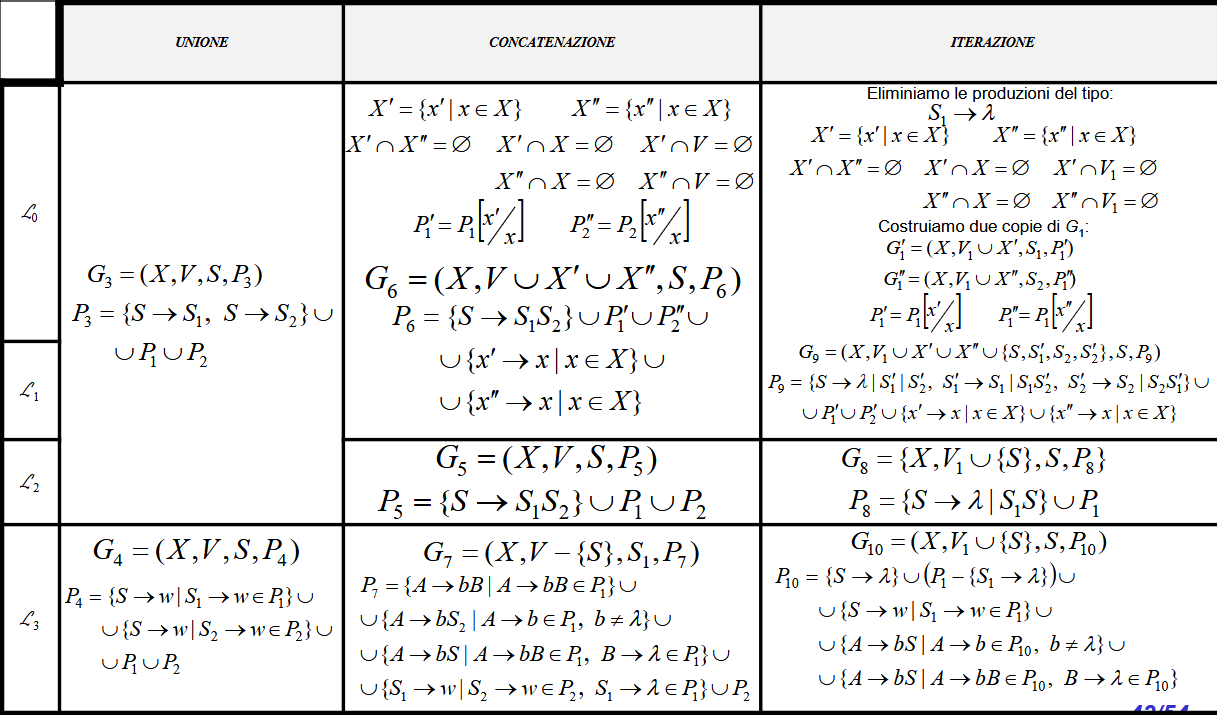
\includegraphics[width=1.00\textwidth]{teoremi_chiusura}
	\end{figure}
	\subsection{Altri teoremi di chiusura}
	\begin{itemize}
		\item La classe dei linguaggi \textit{lineari destri}, di tipo '3'\textbf{chiusa} rispetto al \textit{complemento} e all'\textit{intersezione};
		\item La classe dei linguaggi \textit{non contestuali}, di tipo '2', \textbf{non è chiusa} rispetto al \textit{complemento} e all'\textit{intersezione};
		\item La classe dei linguaggi \textit{contestuali}, di tipo '1' è \textbf{chiusa} rispetto al \textit{complemento} e all'\textit{intersezione};
		\item La classe dei linguaggi di tipo '0' \textbf{non è chiusa} rispetto al \textit{complemento}.
	\end{itemize}
	{
	\proof{
		\begin{itemize}
			\item La classe dei linguaggi \textit{lineari destri}, di tipo '3'\textbf{chiusa} rispetto al \textit{complemento} e all'\textit{intersezione}. \\
			Dimostreremo prossimamente la chiusura di $\mathcal{L}_3$ rispetto al complemento. Dimostriamola rispetto all'intersezione: \\
			Per le leggi di De Morgan:
			\[
			L_1 \cap L_2 = \overline{\overline{L_1} \cup \overline{L_2}}
			\]
			La chiusura di $\mathcal{L}_3$ rispetto all'intersezione discende direttamente da questo risultato.
			\item La classe dei linguaggi \textit{non contestuali}, di tipo '2', \textbf{non è chiusa} rispetto al \textit{complemento} e all'\textit{intersezione}. \\
			Consideriamo i linguaggi:
			\[
			L_1 = \{a^nb^nc^m \mid n, m > 0\} \quad L_2 = \{a^nb^mc^m\mid n, m > 0\}
			\]
			$L_1$ e $L_2$ sono linguaggi liberi, mentre $L_1 \cap L_2$ non lo è:
			\[
			L_1 \cap L_2 = \{a^kb^kc^k \mid k>0\}
			\]
			Il complemento è: $L_1 \cap L_2 = \overline{\overline{L_1} \cup \overline{L_2}}$. \\
			Dunque se $L_1, L_2 \in \mathcal{L}_2$ e se $\mathcal{L}_2$ fosse chiusa rispetto al complemento, $\mathcal{L}_2$ sarebbe chiusa rispetto all'intersezione. 
			\item La classe dei linguaggi \textit{contestuali}, di tipo '1' è \textbf{chiusa} rispetto al \textit{complemento} e all'\textit{intersezione}. \\
			Un risultato recente ha stabilito che $\mathcal{L}_1$ è chiusa rispetto al complemento e quindi all'intersezione. Non se ne conosce la dimostrazione.
			\item La classe dei linguaggi di tipo '0' \textbf{non è chiusa} rispetto al \textit{complemento}. \\
			Non lo dimostriamo.
		\end{itemize}
	}
	}
	\section{Operazione di riflessione}
	{
	\definition[Stringa riflessa]{Sia $w$ una parola su un alfabeto $X = \{x_1, x_2, \dots, x_k\}, w=x_{i_1}, x_{i_2}, \dots,x_{i_{n-1}}, x_{i_n}$. Dicesi \textit{\textbf{stringa riflessa o riflessione}} di $w$ la stringa:
	\[
	w^R = x_{i_n}x_{i_{n-1}}\dots x_{i_2}x_{i_1}
	\]
	}
	\definition[Operazione di riflessione]{Sia $w$una parola su un alfabeto $X = \{x_1, x_2, \dots, x_k\}$ e sia $w^R$ la stringa riflessa di $w$. L'operazione che trasforma $w$ in $w^R$ è detta \textit{\textbf{operazione di riflessione}}}.	
	
	\definition[Parola palindromica]{Un \textit{\textbf{palindromo}} o \textit{\textbf{parola palindromica}} è una parola la cui lettura a ritroso riproduce la parola di partenza:
	\[
	w\ \text{palindromo} \overset{def}{\iff} w = w^R	
	\]
	Un palindromo è dunque una parola che coincide con la sua riflessione.
	}
	}
	I palindromi, su un qualunque alfabeto, sono di due tipi:
	\begin{itemize}
		\item palindromi di lunghezza pari: hanno un asse di simmetria costituito dalla parola vuota;
		\item palindromi di lunghezza dispari: hanno un asse di simmetria costituito da uno dei simbolo dell'alfabeto.
	\end{itemize}
	Più precisamente, si ha la seguente caratterizzazione:
	{
	\theorem{
	Sia $w$ una parola su un alfabeto $X$. $w$ è palindromo se e solo se:
	\[
	w = \alpha x \alpha^R, x \ in X \cup \{\lambda\}
	\]
	Ad esempio:
	\begin{itemize}
		\item $w = alla \quad \alpha = al \quad x = \lambda \quad \alpha^R=la$
		\item $w = radar \quad \alpha = ra \quad x = d \quad \alpha^R = ar$
	\end{itemize}
	}
	\theorem{
	La classe dei linguaggi non contestuali, di tipo '2' è chiusa rispetto all'operazione di riflessione. 
	\proof{
	Sia $G_1 = (X, V_1,S_1, P_1)$ una grammatica non contestuale. \\
	Dobbiamo dimostrare che:
	\[
	L(G_1)\ \text{non contestuale} \Rightarrow (L(G_1))^R = \{w^R \mid L(G_1)\}\ \text{è non contestuale}
	\]
	Costruiamo la grammatica: $G_{11} = (X, V_1, S_1, P_{11})$ ove:
	\[
	P_{11} = \{A \to w^R \mid A \to w \in P_1\}
	\]
	Risulta allora: $L(G_{11}) = (L(G_1))^R$. \\
	Quindi se in $P_1$ abbiamo la produzione: $A \to BaC$ in $P_{11}$ avremo la produzione: $A\to CaB$
	}
	}
	}
	
	\begin{figure}[H]
		\centering
		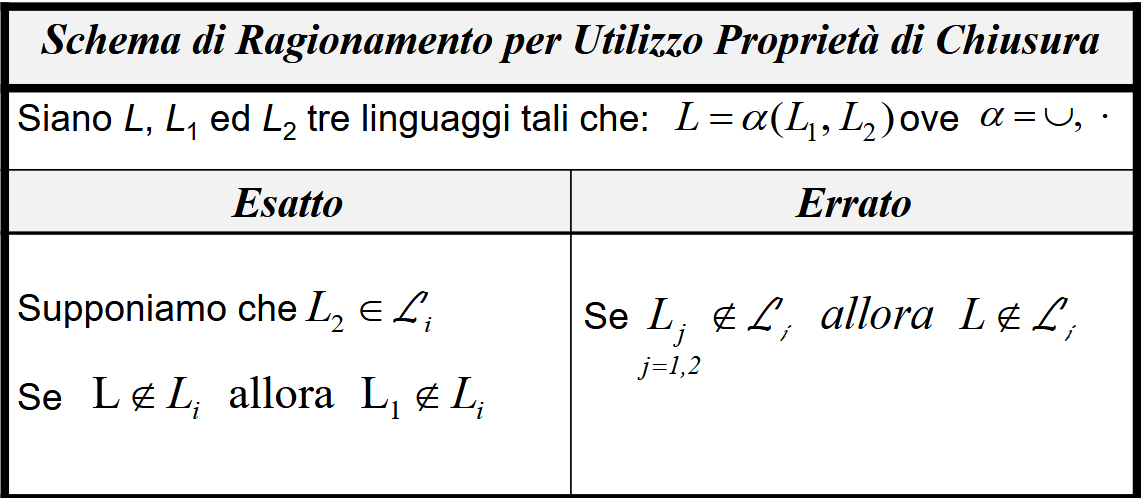
\includegraphics[width=1.00\textwidth]{schema_di_ragionamento_chiusura}
	\end{figure}
	\chapter{Automi a stati finiti}
	\section{Automi a stati finiti deterministici}
	{
		\definition[Automa a stati finiti o accettore a stati finiti o FSA]{
			Sia $X$ un alfabeto. Un \textbf{automa a stati finiti (FSA)} è una quadrupla:
			\[
				M = (Q, \delta, q_0, F)
			\]
			ove:
			\begin{itemize}
				\item $X$ è detto \textbf{alfabeto di ingresso};
				\item $Q$ è un insieme finito e non vuoto di \textbf{stati};
				\item $\delta$ è una funzione da in $Q$, detta \textbf{funzione di transizione}:
				\[
				\delta: Q \times X \to Q
				\]
				\item $q_0$ è lo \textbf{stato iniziale};
				\item $F \subseteq Q$ è l'insieme degli \textbf{stati di accettazione} o \textbf{finali}.
			\end{itemize}
		}
	}
	Talora i valori della funzione di transizione $\delta$ non sono definiti per tutte le coppie (stato-simbolo di ingresso) (q, x). In tal caso, si dice che $\delta$ è una \textbf{funzione parziale} o definita parzialmente. Questo significa che la lettura di $x$ dà luogo in $q$ ad un comportamento dell'automa che non si ritiene utile descrivere ai fini del riconoscimento (nel senso che produrrebbe stringhe non accettate). \\
	Evidentemente questo fatto può essere descritto in modo equivalente, seguendo la definizione data di automa a stati finiti, passando da $q$, per effetto di $x$, in uno stato dal quale non si possa mai raggiungere uno stato finale, detto \textbf{stato di pozza}.  \\
	\subsection{Rappresentazione di FSA}
	Un FSA può essere rappresentato mediante:
	\begin{itemize}
		\item \textit{\textbf{Grado degli Stati} o \textbf{Diagramma di Transizione} o \textbf{Diagramma di Stato}} \\
		È una rappresentazione grafica in cui:
		\begin{itemize}
			\item ogni stato $q \in Q$ è rappresentato da un cerchio (nodo) con etichetta $q$; 
			\item lo stato iniziale (nodo $q_0$) ha un arco orientato entrante libero, ovvero non proviene da nessun altro nodo;
			\item per ogni stato $q \in Q$ e per ogni simbolo $x$ dell'alfabeto di ingresso, $x \in X$, se $\delta(q, x) = q'$, esiste un arco orientato etichettato con $x$ uscente dal nodo $q$ ed entrante nel nodo $q'$.
			\begin{center}
			
			\begin{tikzpicture}[
				> = stealth,
				shorten > = 1pt,
				auto,
				node distance = 3cm
				]
				
				% Define states
				\node[state] (q) {$q$};
				\node[state] (qprime) [right of=q] {$q'$};
				
				% Define transitions
				\draw[->] (q) to node {$x$} (qprime);
				
			\end{tikzpicture}
			\end{center}
		\end{itemize}
		\item \textbf{\textit{Tavola di transizione}}: \\
		È una tabella in cui sono riportati gli stati sulle righe e i simboli dell'alfabeto di ingresso sulle colonne. \\
		Per ogni coppia (stato-ingresso)si legge nella tavola lo stato successivo:
		\begin{tabular}{c|ccccc}
			$\delta$ & $x_1$ & $x_2$ & $\ldots$ & $\ldots$ & $x_n$ \\
			\hline
			$q_0$ & $q_0^1$ & $q_0^2$ & $\ldots$ & $\ldots$ & $q_0^n$ \\
			$q_1$ & $q_1^1$ & $q_1^2$ & $\ldots$ & $\ldots$ & $q_1^n$ \\
			$\ldots$ & $\ldots$ & $\ldots$ & $\ldots$ & $\ldots$ & $\ldots$ \\
			$\ldots$ & $\ldots$ & $\ldots$ & $\ldots$ & $\ldots$ & $\ldots$ \\
			$q_m$ & $q_m^1$ & $q_m^2$ & $\ldots$ & $\ldots$ & $q_m^n$ \\
		\end{tabular} \\
		dove l'alfabeto di ingresso e l'insieme degli stati sono rispettivamente: $X = \{x_1, x_2, \dots, x_n\}$ e $Q = \{q_0, q_1, \dots, q_m\}$. Quindi si ha che: $\delta(q_i, x_j) = {q_i}^j$ con $q_i, {q_i}^j \in Q$ e $x_j \in X$.
	\end{itemize}
	Si può definire un'estensione della funzione transizione $\delta$ come segue:
	{
		\definition[$\delta^*$ per FSA]{
		Dato un FSA $M = (Q, \delta, q_0, F)$ con alfabeto di ingresso $X$, definiamo per induzione la funzione:
		\[
		\delta^*: Q \times X^* \to Q
		\]
		tale che $\delta^*(q, w)$, per $q \in Q$ e $w \in X^*$, sia lo stato in cui $M$ si porta avendo in ingresso la parola $w$ su $X$ e partendo dallo stato $q$. \\
		$\begin{cases}
			\delta^*(q,\lambda) = q \\
			\delta^*(q,wx) = \delta(\delta^*(q, w), x) 	
		\end{cases}$
		per ogni $q \in Q$, $x \in X$, $w\in X^*$
		}
	}
	La figura sottostante riporta una descrizione grafica della definizione precedente:
	\begin{center}
		\begin{tikzpicture}[
			> = stealth,
			shorten > = 1pt,
			auto,
			node distance = 3cm
			]
			
			% Define states
			\node[state] (q) {$q$};
			\node[state, ellipse] (delta) [right of=q] {$\delta^*(q,w)$};
			\node[state] (final) [right of=delta] {};
			
			% Define transitions
			\draw[->] (q) to node {$w$} (delta);
			\draw[->] (delta) to node {$x$} (final);
			\draw[->] (q) to[bend left=45] node {$w\,x$} (final);
			
		\end{tikzpicture}
	\end{center}
	{
		\definition[Parola accettata]{
		Sia $M = (Q, \delta, q_0, F)$ un FSA con alfabeto di ingresso $X$. Una parola $w \in X^*$ è \textbf{accettata} o \textbf{riconosciuta} da $M$ se, partendo dallo stato iniziale $q_0$, lo stato $q$ in cui l'automa si porta alla fine della sequenza di ingresso $w$ è uno stato finale.
		\[
		w\text{ accettata} \overset{def}{\iff} \delta^*(q_0, w) \in F
		\]
		}
		\definition[Linguaggio accettato]{
		Sia $M = (Q, \delta, q_0, F)$ un FSA con alfabeto di ingresso $X$. Il \textbf{linguaggio accettato} o \textbf{riconosciuto} da $M$ è il seguente sottoinsieme di $X^*$:
		\[
		T(M) = \{w \in X^* \mid \delta^*(q_0, w) \in F\}
		\]
		ovvero l'insieme delle parole accettate da $M$.
		}
		\definition[FSA equivalenti]{
		Sia $M_1 = (Q_1, \delta_1, q_1, F_1)$ e $M_2 = (Q_2, \delta_2, q_2, F_2)$ due FSA di alfabeto di ingresso $X$. $M_1$ ed $M_2$ si dicono \textbf{equivalenti} se:
		\[
		T(M_1) = T(M_2)
		\]
		}
		\definition[Linguaggi a stati finiti]{
		Dato un alfabeto $X$, un linguaggio $L$ su $X$ è un \textbf{linguaggio a stati finiti} o (FSL - Finite State Language) se esiste un FSA $M$ con alfabeto di ingresso $X$ tale che $L = T(M)$
		}
		\definition[Classe dei linguaggi a stati finiti]{La \textbf{classe dei linguaggi a stati finiti} è definita come segue:
		\[
		\mathcal{L}_{FSL} = \{L \in 2^{X^*} \mid \exists M, M \text{ è un FSA}: L = T(M)\}
		\]
		}
	}
	{
		\theorem{I linguaggi a stati finiti sono \textbf{chiusi} rispetto al \textbf{complemento}
		\proof{
		Sia $L \in \mathcal{L}_{FSL}$ un linguaggio a stati finiti sull'alfabeto $X$. \\
		Dalla definizione di linguaggio a stati finiti, $L = T(M)$, ove $M = (Q, \delta, q_0, F).$ \\
		Consideriamo il complemento di $L: \overline{L} = X^* - L$ e l'automa a stati finiti $\overline{M} = (Q, \delta, q_0, Q - F)$. Si ha: $\overline{L}=T(\overline{M})$ e questo si dimostra per induzione sulla lunghezza di una parola $w$. \\
		$M$ è un automa a stati finiti con funzione di transizione $\delta$ \textbf{definita totalmente} sul proprio dominio.
		}
		}
	}
	\section{Automi a stati finiti non deterministico o accettore a stati finiti non deterministico}
	{
	\definition[Automa a stati finiti non deterministico]{
	Un \textbf{automa a stati finiti non deterministico} (NDA) con alfabeto di ingresso $X$ è una quadrupla:
	\[M = (Q, \delta, q_0, F)\]
	ove:
	\begin{itemize}
		\item per $Q, q_0, F$ valgono le definizioni date per gli FSA;
		\item $\delta: Q \times X \to 2^Q$ è la funzione di transizione che assegna ad ogni coppia $(q, x)$ un insieme $\delta(q, x) \subseteq Q$ di possibili stati successivi.
	\end{itemize}
	}
	}
	Un NDA è un FSA con l'unica eccezione che, in corrispondenza di una coppia $(q,x)$, vi è un insieme di stati in cui l'automa può transitare. \\
	Come per gli FSA si può definire un'estensione della funzione di transizione $\delta$ come segue:
	{
		\definition[$\delta^*$ per NDA]{
		Dato un NDA $M = (Q, \delta, q_0, F)$ con alfabeto di ingresso \textit{X}, definiamo per induzione la funzione: 
		\[
		\delta^*: 2^Q \times X^* \to 2^Q
		\]
		$\begin{cases}
			\delta^*(p, \lambda) = p \\
			\delta^*(p, wx) = \mathlarger{\bigcup_{q \in \delta^*(p, w)}}
		\end{cases} \quad \forall p \in 2^Q\ (p \subset Q), x \in X, w \in X^*$ 
		}
	}
	Analogamente a quanto fatto per gli FSA, si dovrebbero riformulare le definizioni di parola accettata e di linguaggio accettato da un NDA. \\
	La complicazione, rinveniente dalla computazione non deterministica dello stato successivo in cui un NDA transita, comporta che una stessa parola può indurre cammini multipli attraverso un NDA, alcuni che terminano in stati di accettazione, altri che terminano in stati di non accettazione.
	{
	\definition[Parola accettata da un NDA]{
	Sia $M = (Q, \delta, q_0, F)$ un NDA con alfabeto di ingresso $X$. Una parola $w \in X^*$ è \textbf{accettata} da $M$ se, partendo dallo stato iniziale $q_0$, esiste almeno un modo per $M$ di portarsi in uno stato di accettazione alla fine della sequenza di ingresso $w$. In formule:
	\[
	w\ accettata\ \overset{def}{\iff} \exists p: p \in \delta^*(\{q_0\}, w) \cap F \iff \delta^*(\{q_0\}) \cap F \neq \emptyset
	\]
	}
	}
	Vedere gli esempi dalle slide. \\
	{
	\definition[Linguaggio accettato da un NDA]{
	Sia $M = (Q, \delta, q_0, F)$ un NDA con alfabeto di ingresso $X$. Il \textbf{linguaggio accettato} o \textbf{riconosciuto} da $M$ è l'insieme della parole su $X$ accettate da $M$:
	\[
	T(M) = \{w \in X^* \mid \delta^*(\{q_0\}, w) \cap F \neq \emptyset\}
	\]
	}
	ovvero l'insieme della parole $w$ per le quali esiste almeno un cammino, etichettato con lettere di $w$ nell'ordine da sinistra a destra, attraverso il diagramma degli stati che porta $M$ dallo stato iniziale ad uno degli stati di accettazione.
	\definition[NDA equivalenti]{
	Siano $M_1 = (Q_1, \delta_1, q_1, F_1)$ ed $M_2 = (Q_2, \delta_2, q_2, F_2)$ due NDA di alfabeto di ingresso $X$. $M_1$ ed $M_2$ si dicono \textbf{equivalenti} se:
	\[
	T(M_1) = T(M_2)
	\]
	}
	\definition[Classe dei linguaggi riconosciuti da automi a stati finiti non deterministici]{
	Di seguito la definizione della \textbf{classe dei linguaggi riconosciuti da automi a stati finiti non deterministici: 
	\[
	\mathcal{L}_{NDL} = \{L \in 2^{X^*} \mid \exists M, M \text{è un NDA}: L = T(M)\}
	\]
	}
	}
	}
	\section{Equivalenza delle classi di linguaggi accettati da automi a stati finiti deterministici e non deterministici}
	{
	\theorem[Equivalenza delle classi di linguaggi accettati da automi a stati finiti deterministici e non deterministici]{
	\begin{itemize}
		\item Le classi di linguaggi $\mathcal{L}_{FSL}$ e $\mathcal{L}_{NDL}$ sono equivalenti ($1^a$ formulazione).
		\item Sia $L$ un linguaggio su $X$. $L$ è un linguaggio a stati finiti se e solo se $L = T(M)$ per qualche NDA $M$ ($2^a$ formulazione)
	\end{itemize} 
	\proof[$2^a$ formulazione] \quad \\
	$\implies)$ Sia $L \in 2^{X^*}$ ed $L \in \mathcal{L}_{FSL}$. Dalla definizione di linguaggi a stati finiti si ha: 
	\[
	\exists M_1: M_1 \text{ è un FSA, } M_1 = (Q_1, \delta_1, F_1)
	\]
	con alfabeto di ingresso $X: L = T(M_1)$. \\
	Sulla base di $M_1$, definiamo il seguente $NDA$ con alfabeto di ingresso $X$:
	\[
	M_2 = (Q_2, \delta_2, q_2, F_2)
	\]
	ove:
	\begin{itemize}
		\item $Q_2 = Q_1$;
		\item $\delta_2$ è cosi definita:
		\[
		\delta_2: Q_2 \times X \to 2^{Q_2},
		\]
		\[
		\delta_2(q,x) = \{q_1(q, x)\} \quad \forall q \in Q_2 = Q_1, x \in X
		\]
		\item $q_2 = q_1$;
		\item $F_2 = F_1$.
	\end{itemize}
	$M_2$ è un NDA ed inoltre accetta lo stesso linguaggio accettato da $M_1$, ossia si ha: $T(M_2) = T(M_1)$. \\
	$\Leftarrow)$ Sia $L \in 2^{X^*}$ ed $L \in \mathcal{L}_{NDL}$. Dalla definizione della classe di linguaggi $\mathcal{L}_{NDL}$, si ha:
	\[
	\exists M, \text{M è un NDA, } M = (Q, \delta, q_0, F)
	\]
	con alfabeto di ingresso $X: L=T(M)$. \\
	Si può definire allora il seguente algoritmo per la costruzione di un FSA equivalente all'NDA $M$: \\
	Sia $M = (Q, \delta, q_0, F)$ un automa a stati finiti non deterministico di alfabeto di ingresso $X$. $M$ può essere trasformato in un automa deterministico $M'$ di alfabeto di ingresso $X$ come segue: $M'=(Q', \delta', q_0', F')$ ove:
	\begin{itemize}
		\item $Q'=2^Q$
		\item $q_0'=\{q_0\}$
		\item $F' = \{ p \subseteq Q \mid p \cap F \neq \emptyset\}$
		\item $\delta': Q'\times X \to Q' \quad \forall q'= \{q_1, q_2, \dots, q_i\} \in Q', \forall x \in X$:
		\[
		\delta'(q', x) = \delta'(\{q_1, q_2, \dots, q_i\}, x) = \mathlarger{\bigcup_{j=1}^i\delta}(q_j, x) = \mathlarger{\bigcup_{q \in q'}}\delta(q, x).
		\]
	\end{itemize}
	Si può dimostrare che $M'$ è equivalente a $M$, ossia che:
	\[
	T(M')=T(M)
	\]
	}
	}
	\chapter{Linguaggi regolari, espressioni regolari e teorema di Kleene}
	\begin{figure}[H]
		\centering
		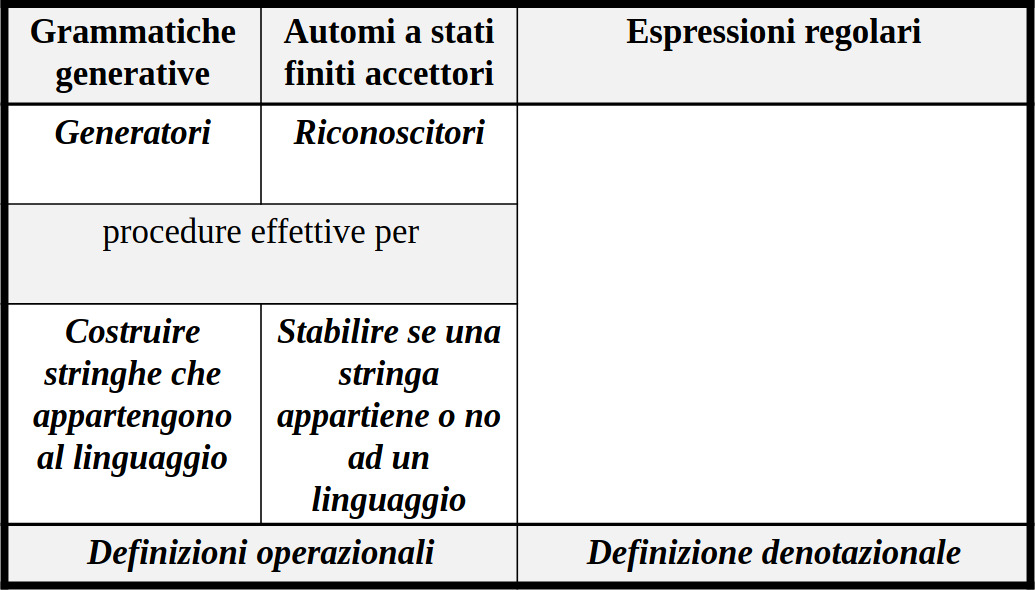
\includegraphics[width=1.00\textwidth]{descrizione_linguaggi_destri}
		\caption{Descrizione algebrica dei linguaggi lineari destri}
	\end{figure}
	\section{Linguaggi regolari ed espressioni regolari}
	{
	\definition[Linguaggio regolare]{
	Sia $X$ un alfabeto. Un linguaggio $L \subset X^*$ è \textbf{regolare} se:
	\begin{itemize}
		\item $L$ è finito, $(|L| = k, k$ intero)
	\end{itemize}
	oppure se:
	\begin{itemize}
		\item $L$ può essere ottenuto per induzione, sulla costruzione, utilizzando una delle seguenti operazioni:
		\begin{itemize}
			\item $L = L_1 \cup L_2$, con $L_1, L_2$ regolari;
			\item $L = L_1 \cdot L_2$, con $L_1, L_2$ regolari;
			\item $L = L_1^*$ con $L_1$ regolare.
		\end{itemize}
	\end{itemize}
	Si noti che $\emptyset$ e $\{\lambda\}$ sono linguaggi regolari. \\
	Denotiamo con $\mathcal{L}_{REG}$ la classe dei linguaggi regolari.
	}
	\definition[Espressione regolare]{Sia $X$ un alfabeto. Una stringa $R$ di alfabeto $X \cup \{\lambda, +, *, \cdot, \emptyset, (, )\}$, con $X \cap \{\lambda, +, *, \cdot, \emptyset, (, )\} = \emptyset$ è una \textbf{espressione regolare} di alfabeto $X$ se e solo se vale una delle seguente condizioni:
	\begin{itemize}
		\item $R = \emptyset$
		\item $R = \lambda$ 
		\item $R = a$, $\forall a \in X$
		\item $R = (R_1 + R_2)$ con $R_1, R_2$ espressioni regolari di alfabeto $X$
		\item $R = (R_1 \cdot R_2)$ con $R_1, R_2$ espressioni regolari di alfabeto $X$
		\item $R = (R_1)^*$ con $R_1$ espressione regolare di alfabeto $X$
	\end{itemize}
	}
	}
	Ad ogni espressione regolare $R$ corrisponde un linguaggio regolare $S(R)$ definito nel seguente modo: \\
	\begin{tabular}{|c|c|}
		\hline
		\textbf{\textit{Espressione regolare}} & \textbf{\textit{Linguaggio regolare corrispondente}}  \\
		\hline
		$\emptyset$ & $\emptyset$ \\
		\hline
		$\lambda$ & $\{\lambda\}$ \\
		\hline
		$a$ & $\{a\}$ \\
		\hline
		$(R_1 + R_2)$ & $S(R_1) \cup S(R_2)$ \\
		\hline
		$(R_1 \cdot R_2)$ & $S(R_1) \cdot S(R_2)$ \\
		\hline
		$(R_1)^*$ & $(S(R_1))^*$ \\
		\hline
	\end{tabular}
	{
		\definition[Linguaggio regolare]{Un linguaggio su $X$ è regolare se e solo se corrisponde ad una espressione regolare su $X$. Quindi, denotato con $\mathfrak{R}$ l'insieme delle espressioni regolari di alfabeto $X$, definiamo la funzione:
		\[
		S: \mathfrak{R} \to 2^{X^*}
		\]
		che ad ogni espressione regolare $R$ associa il corrispondente linguaggio regolare $S(R)$. Si ha dunque: \[
		\mathcal{L}_{REG} = \{L \in 2^{X^*} \mid \exists R \in \mathfrak{R}, L = S(R)\}
		\]
		}
	}
	Un linguaggio regolare può essere descritto da più di una espressione regolare, ossia $S: \mathfrak{R} \to 2^{X^*}$ non è una funzione iniettiva. \\
	Ad esempio il linguaggio costituito da tutte le parole su $X = \{a, b\}$ con $a$ e $b$ che si alternano e che hanno come suffisso e prefisso $b$ può essere descritto sia dall'espressione regolare:
	\[
	b\cdot(ab)^*
	\]
	sia da:
	\[
	(ba)^*b
	\]
	{
	\definition[Espressioni regolari equivalenti]{
	Due espressioni regolari $R_1$ e $R_2$ su $X$ sono \textbf{equivalenti}, ovvero $R_1 = R_2 \iff S(R_1) = S(R_2)$
	}
	}
	\subsection{Proprietà delle espressioni regolari}
	Siano $R_1, R_2$ ed $R_3$ espressioni regolari di alfabeto $X$, risulta:
	\begin{enumerate}
		\item $(R_1 + R_2) + R_3 = R_1 + (R_2 + R_3) = R_1 + R_2 + R_3$ \textbf{proprietà associativa} 
		\item $R_1 + R_2 = R_2 + R_1$ \textbf{proprietà commutativa}
		\item $R_1 + \emptyset = \emptyset + R_1 = R_1$ ovvero $\emptyset$ è l'elemento neutro rispetto all'operazione $+$
		\item $R_1 + R_1 = R_1$ \textbf{proprietà idempotenza} 
		\item $(R_1 \cdot R_2) \cdot R_3 = R_1 \cdot (R_2 \cdot R_3) = R_1 \cdot R_2 \cdot R_3$ \textbf{proprietà associativa}
		\item $R_1 \cdot R_2 \neq R_2 \cdot R_1$
		\item $R_1 \cdot \lambda = \lambda \cdot R_1 = R_1$ ovvero $\lambda$ è l'elemento neutro rispetto all'operazione $\cdot$
		\item $R_1 \cdot \emptyset = \emptyset \cdot R_1 = \emptyset$ ovvero $\emptyset$ è l'elemento assorbente rispetto all'operazione $\cdot$
		\item $R_1 \cdot (R_2 + R_3) = (R_1 \cdot R_2) + (R_1 \cdot R_3)$ \textbf{proprietà distributiva sinistra}
		\item $(R_1 + R_2) \cdot R_3 = (R_1 \cdot R_3) + (R_2 \cdot R_3)$ \textbf{proprietà distributiva destra}
		\item $(R_1)^* = (R_1)^* \cdot (R_1)^* = ((R_1)^*)^* = (\lambda + R_1)^*$
		\item $(\emptyset)^* = (\lambda)^* = \lambda$
		\item $(R_1)^* = \lambda + R_1 + R_1^2 + \dots + R_1^n + (R_1^{n+ 1} \cdot R_1^*)$ \\
		\textbf{Caso particolare:} \\
		$(R_1)^* = \lambda + R_1 \cdot R_1^* = \lambda + R_1^* \cdot R_1$
		\item $(R_1 + R_2)^* = (R_1^* + R_2^*)^* = (R_1^* \cdot R_2^*)^* = (R_1^* \cdot R_2)^* \cdot R_1^* = R_1^* \cdot (R_2 \cdot R_1^*)^*$
		\item $(R_1 + R_2)^* \neq R_1^* + R_2^*$
		\item $R_1^* \cdot R_1 = R_1 \cdot R_1^*$
		\item $R_1 \cdot (R_2 \cdot R_1)^* = (R_1 \cdot R_2)^* \cdot R_1$
		\item $(R_1^* \cdot R_2)^* = \lambda + (R_1 + R_2)^* \cdot R_2$
		\item $(R_1 \cdot R_2^*)^* = \lambda + R_1 \cdot (R_1 + R_2)^*$
		\item Supponiamo che: $\lambda \notin S(R_2)$ \\
		$R_1 = R_2 \cdot R_1 + R_3 \iff R_1 = R_2^* \cdot R_3$ \\
		$R_1 = R_1 \cdot R_2 + R_3 \iff R_1 = R_3 \cdot R_2^*$ 
	\end{enumerate}
	Dimostriamo la proprietà 17 mediante la tecnica di \textbf{riparsificazione}: 
	\[
	R_1 \cdot (R_2 \cdot R_1)^* = (R_1 \cdot R_2)^* \cdot R_1
	\]
	Si consideri dunque la parola:
	\[
	w \in S(R_1 \cdot (R_2 \cdot R_1)^*), w = r_1^0(r_2^1 \cdot r_1^1) \cdot (r_2^2 \cdot r_1^2) \cdot \dots \cdot (r_2^n \cdot r_1^n), n \geq 0
	\]
	ove:
	\[
	r_1^i \in S(R_1) \quad i = 0, 1, 2, \dots, n
	\]
	\[
	r_2^j \in S(R_2) \quad j = 0, 1, 2, \dots, n
	\]
	Riparsificando $w$ ed utilizzando la proprietà associativa della concatenazione, si ha: $w = (r_1^0 \cdot r_2^1) \cdot (r_1^1 \cdot r_2^2) \cdot \dots \cdot (r_1^{n-1} \cdot r_2^n) \cdot r_1^n$, dunque $w \in S((R_1 \cdot R_2)^*\cdot R_1)$ da cui: $S(R_1 \cdot (R_2 \cdot R_1)^*) \subseteq S((R_1 \cdot R_2)^*\cdot R_1)$ \\
	In modo analogo si dimostra: $S(R_1 \cdot (R_2 \cdot R_1)^*) \supseteq S((R_1 \cdot R_2)^* \cdot R_1)$ \\
	Un'altra tecnica comune per dimostrare tali proprietà è semplicemente quella di utilizzare proprietà già note. \\
	Mostreremo ora come si usano le proprietà delle espressioni regolari per provare l'equivalenza di espressioni regolari. \\
	\textbf{Esercizio: applicazione delle proprietà per semplificare espressioni regolari} \\
	Dimostrare la seguente equivalenza:
	\[
	(b + aa^*b) + (b + aa^*b) \cdot (a + ba^*b) \cdot (a + ba^*b) = a^*b \cdot (a + ba^*b)^*
	\]
	$(b + aa^*b) + (b + aa^*b) \cdot (a + ba^*b) \cdot (a + ba^*b) = (b + aa^*b) \cdot [\lambda + (a + ba^*b)^*(a + ba^*b)]$ \\
	Per la proprietà 13. $(R_1)^* = \lambda + R_1 \cdot R_1^* = \lambda + R_1^* + R_1$, quindi: \\
	$(b + aa^*b) \cdot [\lambda + (a + ba^*b)^*(a + ba^*b)] = (b + aa^*b) \cdot (a + ba^*b)^* = (\lambda + aa^*)\cdot b \cdot (a + ba^*b)^* = a^*b \cdot (a + ba^*b)^*$
	\section{Teorema di Kleene}
	{
		\theorem[Teorema di Kleene]{
		$\mathcal{L}_3 \equiv \mathcal{L}_{FSL} \equiv \mathcal{L}_{REG}$ \\
		Equivalenza tra: linguaggi lineari destri, linguaggi a stati finiti, linguaggi regolari. \\
		\begin{figure}[H]
			\centering
			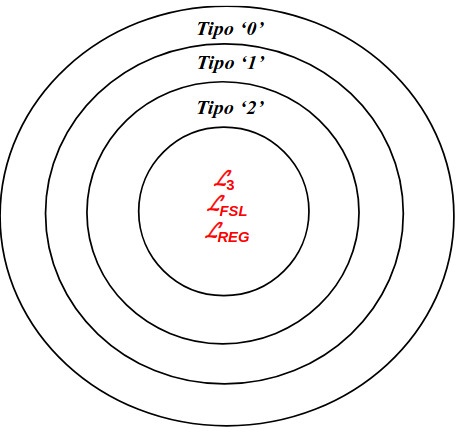
\includegraphics[width=0.40\textwidth]{teorema_kleene}
		\end{figure}
		\proof[Dimostrazione teorema di Kleene]{
		Lo schema della dimostrazione è il seguente:
		\begin{itemize}
			\item $\mathcal{L}_3 \subset \mathcal{L}_{FSL} \quad (\mathcal{L}_{FSL} \subset \mathcal{L}_3)$
			\item $\mathcal{L}_{FSL} \subset \mathcal{L}_{REG}$
			\item $\mathcal{L}_{REG} \subset \mathcal{L}_3$
		\end{itemize}
		\begin{itemize}
			\item $\mathcal{L}_3 \subset \mathcal{L}_{FSL}$ \\
			Sia $L \in \mathcal{L}_3 \iff \exists G = (X, V, S, P), G$ di tipo '3': $L(G) = L$ \\
			Vogliamo costruire un automa a stati finiti:
			\[
			M = (Q, \delta, q_0, F) \text{ tale che } T(M) = L(G)
			\]
			Allo scopo si fornisce il seguente algoritmo per la costruzione di un automa a stati finiti non deterministico che riconosce il linguaggio generato da una fissata grammatica lineare destra. \\
			Data una grammatica lineare destra: 
			\[
			G = (X, V, S, P)
			\]
			l'automa accettore a stati finiti equivalente $T(M) = L(G)$ viene costruito come segue:
			\[
			M = (Q, \delta, q_0, F)
			\]
			\begin{itemize}
				\item $X$ come alfabeto di ingresso;
				\item $Q = V \cup \{q\}, q \notin V$
				\item $q_0 = S$
				\item $F = \{q\} \cup \{B \mid B \to \lambda \in P\}$
				\item $\delta: Q \times X \to 2^Q \quad$ \begin{align*}
					V. a \quad \forall B \to aC \in P, C \in \delta(B, a) \\
					V. b \quad \forall B \to a \in P, q \in \delta(B, a)
				\end{align*}
			\end{itemize}
			L'algoritmo può generare un automa non deterministico per effetto dei passi $V.a$ e $V.b$. Si può facilmente constatare che, se: $w = x_1x_2\dots x_n \in L(G)$ $w$ può essere generata da una derivazione del tipo: 
			\[
			S \Rightarrow x_1X_2 \Rightarrow x_1x_2X_3 \Rightarrow \dots \Rightarrow x_1x_2\dots x_{i-1}X_i \Rightarrow x_1x_2\dots x_i
			\]
			Dalla definizione data, l'automa $M$, esaminando la stringa $w = x_1x_2\dots x_n$ compie una serie di mosse che lo portano dallo stato $S$ ad $X_1, X_2, \dots , X_i$ e $q$; pertanto $L(G) \subseteq T(M)$. \\
			In modo del tutto analogo, ogni $w$ in $T(M)$ comporta una sequenza di mosse dell'automa a cui corrisponde una derivazione in $G$, e pertanto $T(M) \subseteq L(G)$ \\
			Se ne deduce che: $L(G) = T(M)$ \\
			Sebbene non sia strettamente necessario per la dimostrazione del Teorema di Kleene, per il suo interesse pratico si riporta di seguito l'algoritmo per la costruzione di una grammatica lineare destra che genera il linguaggio accettato da un automa a stati finiti. \\
			Tale algoritmo costruisce una dimostrazione costruttiva del seguente risultato:
			\[
			\mathcal{L}_{FSL} \subset \mathcal{L}_3
			\]
			Sia dato un automa accettore a stati finiti: 
			\[
			M = (Q, \delta, q_0, F)
			\]
			con alfabeto di ingresso $X$. \\
			La grammatica lineare destra $G$ equivalente a $M$, ossia tale che $L(G) = T(M)$, si costruisce come segue:
			\begin{itemize}
				\item $X = $ alfabeto di ingresso di $M$
				\item $V = Q$
				\item $S = q_0$
				\item $P = \{q \to xq' \mid q' \in \delta(q, x)\} \cup \{q \to x \mid \delta(q, x) \in F\} \cup \{q_0 \to \lambda \mid q_0 \in F\}$
			\end{itemize}
		\end{itemize}
		}
		}
	}
	\section{Pumping Lemma per i linguaggi regolari}
	{
	\theorem[Pumping Lemma per i linguaggi regolari]{
	Sia $M = (Q, \delta, q_0, F)$ un automa accettore a stati finiti con $n$ stati ($|Q| = n$) e sia $z \in T(M), |z| \geq n$. \\
	Allora $z$ può essere scritta come $uvw$ e $uv^*w \subset T(M)$ ossia $\forall i, i \geq 0: uv^iw \in T(M)$. \\
	Una formulazione alternativa è la seguente: \\
	Sia $L = T(M)$ un linguaggio regolare con $M = (Q, \delta, q_0, F)$ un automa accettore a stati finiti. \\
	Allora $\exists n = |Q| \mid \forall z \in L, |z| \geq n: z = uvw$ e:
	\begin{itemize}
		\item $|uv| \leq n$
		\item $v \neq \lambda$
		\item $uv^iw \in L, \forall i, i \geq 0$
	\end{itemize} 
	\proof{
	Sia $z = x_1x_2\dots x_k, z \in T(M)$ \\
	Possiamo rappresentare il comportamento dell'automa $M$, con ingresso $z$, come segue: 
	\begin{figure}[H]
		\centering
		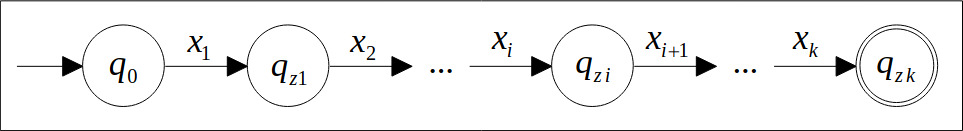
\includegraphics[width=1.00\textwidth]{pumping_lemma_liberi}
	\end{figure}
	Se si ha: $|z| \geq n$, nella figura devono comparire almeno $n+1$ stati ma, poichè $M$ ha solo $n$ stati distinti, almeno uno stato tra $q_0, q_{z1}, q_{z2}, \dots, q_{zk}$ deve comparire due volte. \\
	Supponiamo che si abbia: $q_{zi} = q_{zj}, i < j$. \\
	Si ha dunque la situazione rappresentata in figura:  
	\begin{figure}[H]
		\centering
		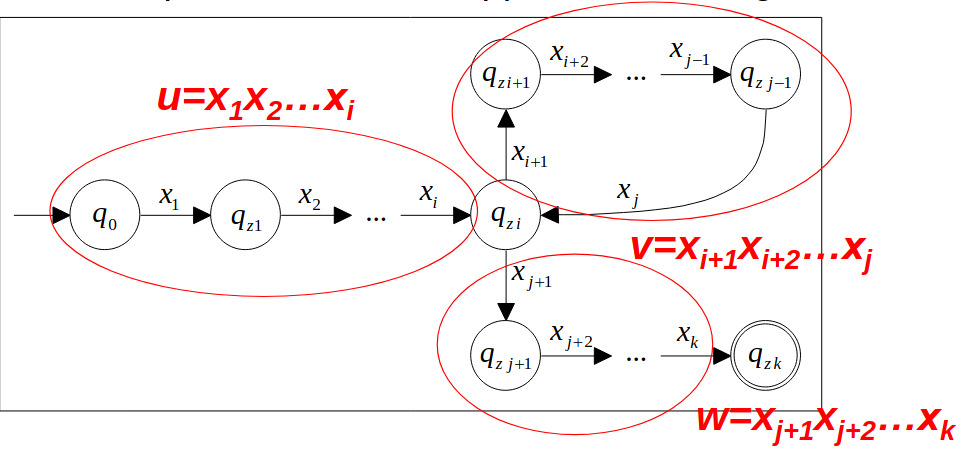
\includegraphics[width=1.00\textwidth]{dim_pumping_lemma_regolari}
	\end{figure}
	Possiamo scrivere $z$ nella forma: $z = uvw$. \\
	Poichè $z \in T(M)$, l'automa $M$, per effetto dell'ingresso di $z=uvw$, si porta per definizione in uno stato finale $(\delta^*(q_0, z)\in F)$. \\
	Ma è immediato osservare che tale stato è lo stesso in cui $M$ si porta per effetto dell'ingresso delle parole $uw$, $uv^2w, \dots, uv^iw, i \geq 0$. \\
	Dunque si ha: $uv^iw \in T(M), i \geq 0$.
	}
	}
	}
	\section{Proprietà decidibili dei linguaggi regolari} 
	Dato $M = (Q, \delta, q_0, F)$ con alfabeto di ingresso $X$: 
	\begin{itemize}
		\item $T(M) = \emptyset$ è decidibile \\
		Per dimostrarlo bisogna provare per tutte le parole $w \in X^*: |w| < |Q|$ 
		\item $T(M) = \infty$ \\
		Per dimostrarlo bisogna provare per tutte le parole $w \in X^*: |Q| \leq |w| < 2^|Q|$
	\end{itemize}
	Dati $M_1 = (Q', \delta', q_0', F')$ e $M_2 = (Q'' , \delta'', q_0'', F'')$ con alfabeto di ingresso $X$:
	\begin{itemize}
		\item $T(M_1) = T(M_2)$ è decidibile. \\
		La dimostrazione discende dalla prima proprietà decidibile in quanto:
		\begin{itemize}
			\item $T(M_1) \backslash T(M_2) = \emptyset$ è decidibile
			\item $T(M_2) \backslash T(M_1) = \emptyset$ è decidibile
		\end{itemize}
		e la classe dei linguaggi regolari è chiusa rispetto alle operazioni di intersezione e complemento.
	\end{itemize} 
	\chapter{Modello di un compilatore}
	La costruzione di un compilatore per un linguaggio di programmazione è un'operazione abbastanza complessa. La complessità dipende principalmente dal linguaggio sorgente. \\
	Un compilatore traduce il programma sorgente in programma oggetto. Le azioni che compie sono:
	\begin{itemize}
		\item \textbf{Analisi} del programma sorgente;
		\item \textbf{Sintesi} del programma oggetto.
	\end{itemize}
	\begin{figure}[H]
		\centering
		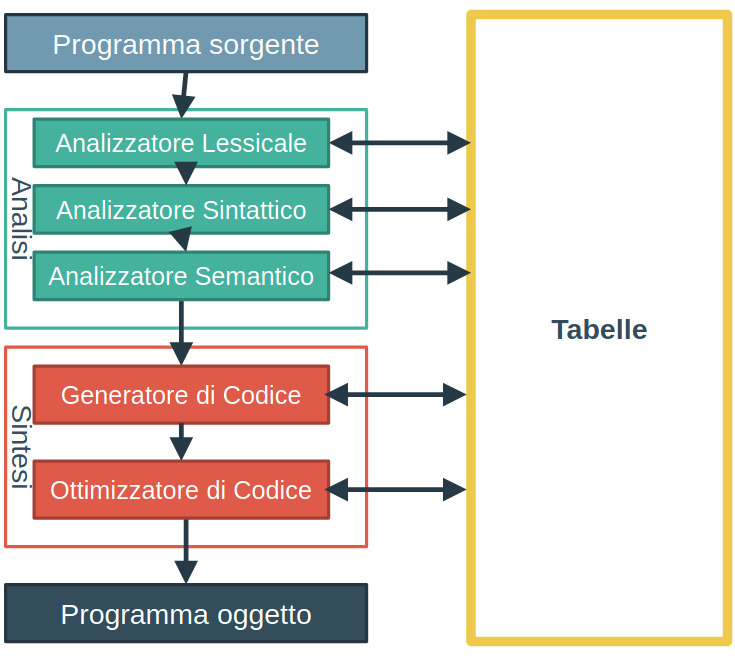
\includegraphics[width=1.00\textwidth]{modello_funzionale_compilatore}
		\caption{Modello funzionale di un compilatore}
	\end{figure}
	Un programma sorgente è una stringa di simboli, ad esempio:
	\[
	\text{if A $>$ B then X:=Y;}
	\]
	\section{Analizzatore lessicale (scanner)}
	Un analizzatore lessicale prende in \textbf{input} un programma sorgente, esamina il programma per individuare i simboli (token), che lo compongono classificando parole chiave, identificatori, operatori, costanti, ecc. \\
	Per ragioni di efficienza ad ogni classe di token è dato un numero unico che la identifica. \\
	Un analizzatore lessicale, dopo che ha compito le sue operazioni, restituisce in \textbf{output} una lista di token. \\
	Ad esempio, data la stringa $\text{if A $>$ B then X:=Y;}$ \\
	\begin{tabular}{c c}
		IF & 20 \\
		A & 1 \\
		> & 15 \\
		B & 1 \\
		THEN & 20 \\
		X & 1 \\
		:= & 10 \\
		Y & 1 \\
		; & 27
	\end{tabular}
	Si noti che vengono ignorati spazi bianchi e commenti. Inoltre alcuni scanner inseriscono label, costanti e variabili in tavole appropriate. \\
	Un elemento della tavola per una variabile, ad esempio, contiene nome, tipo, indirizzo, valore e linea in cui è dichiarata. \\
	\begin{figure}[H]
		\centering
		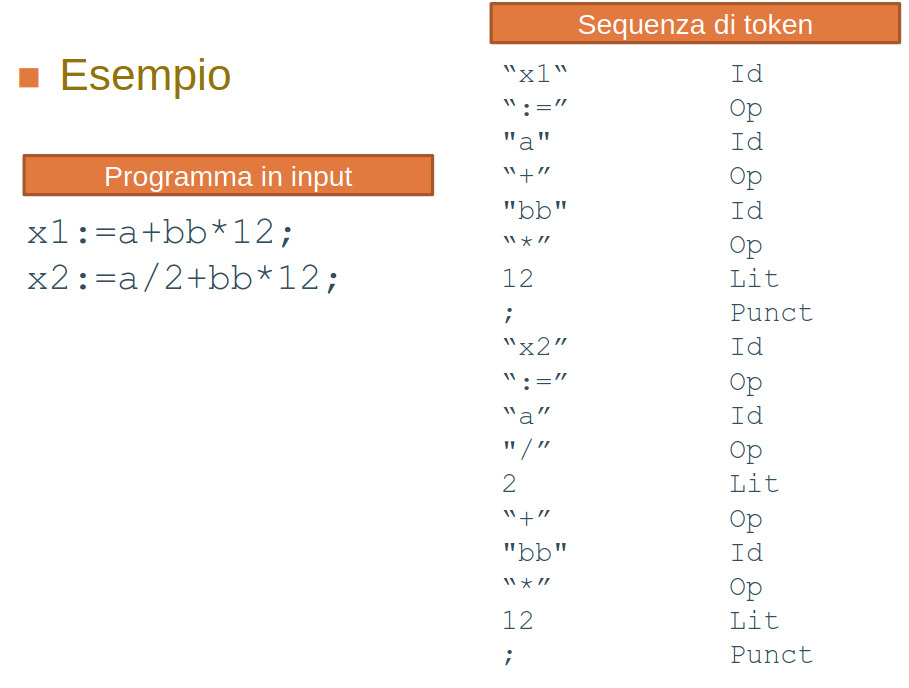
\includegraphics[width=1.00\textwidth]{scanner}
	\end{figure}
	Notare come simboli appartenenti alla stessa classe di token hanno tutti lo stesso tipo, come 'Op', 'Lit' ecc. \\
	\section{Analizzatore sintattico (parser)}
	Un analizzatore sintattico o parser, prende in \textbf{input} una lista di token, individua la struttura sintattica della stringa in esame a partire dal programma sorgente sotto forma di token. Un parser, quindi, identifica espressioni, istruzioni e procedure. Un parser restituisce in \textbf{output} un albero sintattico. \\
	Ad esempio, data la stringa:
	\[
	\text{ALFA1 := 5 + A * B}
	\]
	La stringa 5 + A * B è riconosciuta come: $<$espressione$>$. \\
	La stringa completa è riconosciuta come $<$assegnazione$>$ in accordo alla regola sintattica:
	\[
	<\text{assegnazione}>::= <\text{variabile}> := <\text{espressione}>
	\]
	In realtà si utilizza la stringa semplificata del tipo:
	\[
	\text{id1 := c2 + id3 * id4}
	\]
	con accesso alla rappresentazione generata dallo scanner. \\
	L'analisi della stringa:
	\[
	\text{(A + B) * (C + D)}
	\]
	produce le classi sintattiche:
	\begin{itemize}
		\item $<$fattore$>$
		\item $<$termine$>$
		\item $<$espressione$>$
	\end{itemize}
	Il controllo sintattico si basa sulle \textbf{regole grammaticali} utilizzate per definire formalmente il linguaggio. \\
	Durante il controllo sintattico si genera l'albero di derivazione, l'\textbf{albero sintattico}. \\
	\begin{figure}[H]
		\centering
		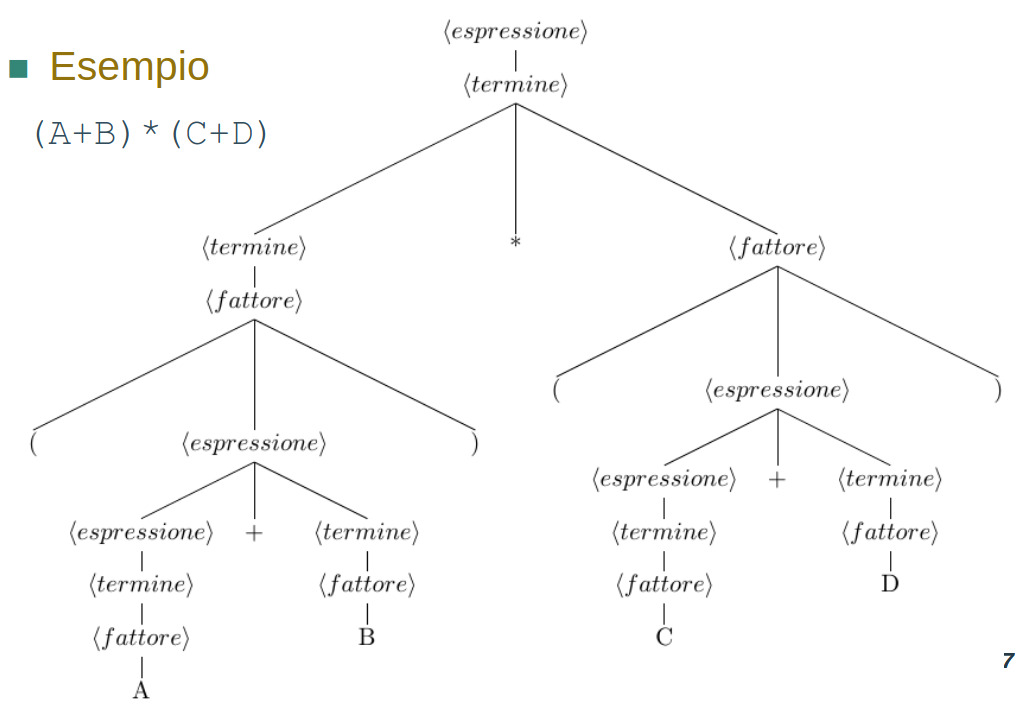
\includegraphics[width=1.00\textwidth]{parser}
	\end{figure}
	\begin{figure}[H]
		\centering
		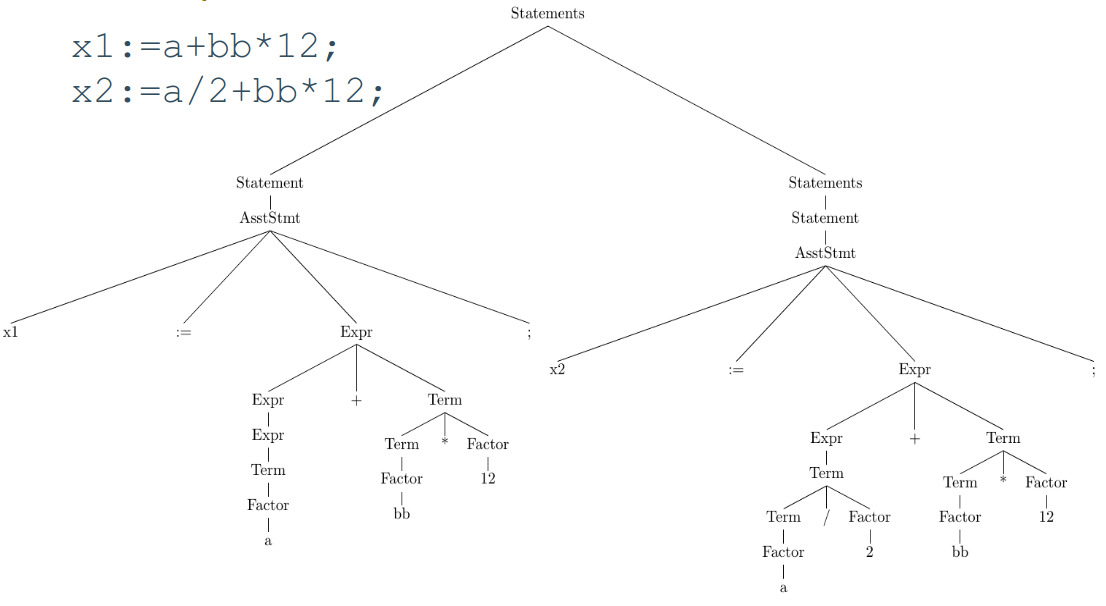
\includegraphics[width=1.00\textwidth]{esempio_parser}
	\end{figure}
	\section{Analizzatore semantico}
	Un analizzatore semantico, prende in \textbf{input} l'albero sintattico generato dal parser. Un analizzatore semantico si compone di due fasi principali:
	\begin{enumerate}
		\item \textbf{Controlli statici}, o static checking. 
		\item \textbf{Generazione di una rappresentazione intermedia} (IR).
	\end{enumerate}
	Un analizzatore semantico restituisce come \textbf{output} un albero arricchito con informazioni sui vincoli sintattici contestuali. \\
	Durante i  \textbf{controlli statici} sono svolti vari controlli sui tipi, dichiarazioni, numero parametri funzioni, ecc. \\
	Per l'espressione (A + B) * (C + D), ad esempio, l'analizzatore semantico deve determinare quali azioni sono specificate dagli operatori aritmetici di addizione e moltiplicazione. \\
	Ad ogni token che corrisponde ad un identificatore di variabile è associato: tipo, luogo di dichiarazione, ecc, memorizzate nella tabella dei simboli. \\
	Quando riconosce il + o il * invoca allora una routine semantica che specifica le azioni da svolgere. Ad esempio, che gli operandi siano stati dichiarati, abbiano lo stesso tipo ed un valore. \\
	La \textbf{generazione di una rappresentazione intermedia} (IR), produce una forma intermedia di codice sorgente. \\
	Ad esempio può produrre il seguente insieme di quadruple per (A + B) * (C + D): 
	\[
	\text{(+, A, B, T1) \\ (+, C, D, T2) \\ (*, T1, T2, T3)}
	\]
	od altri tipi di codice intermedio. \\
	Ad esempio il codice intermedio che rimuove dall'albero sintattico alcune delle categorie intermedie e mantiene solo la struttura essenziale, ovvero l'\textbf{albero sintattico astratto}:
	\begin{itemize}
		\item Tutti i nodi sono token;
		\item Le foglie sono operandi; 
		\item I nodi intermedi sono operatori.
	\end{itemize}
	Spesso a valle dell'analizzatore semantico ci può essere un ottimizzatore del codice intermedio. \\
	\begin{figure}[H]
		\centering
		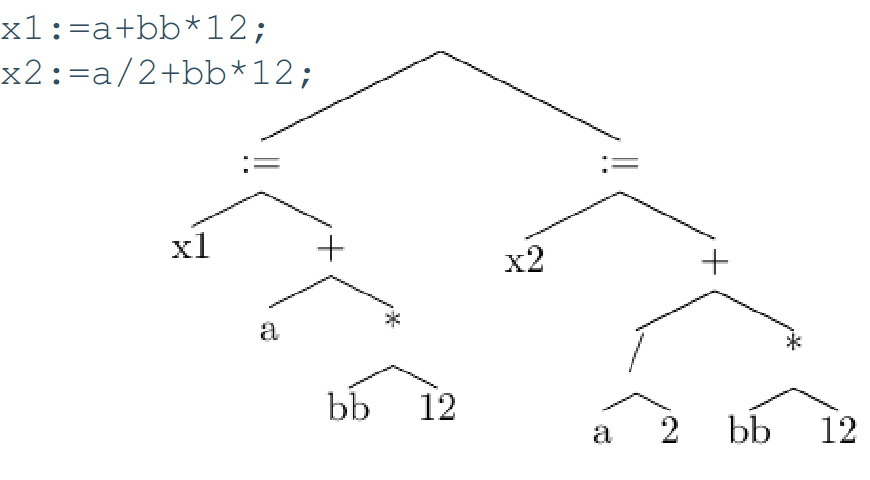
\includegraphics[width=1.00\textwidth]{AST}
		\caption{Esempio dell'albero sintattico astratto}
	\end{figure}
	Per quanto concerne l'ottimizzazione del codice intermedio, questo può avvenire in diversi modi:
	\begin{itemize}
		\item \textbf{Propagazione di costanti}: \\
		Ad esempio:
		\[
		\text{X := 3; \\ A := B + X;}
		\]
		si può ottimizzare come:
		\[
		\text{X := 3; \\ A := B + 3;}
		\]
		evitando un accesso alla memoria.
		\item \textbf{Eliminazione di sotto-espressioni comuni}: \\
		Ad esempio:
		\[
		\text{A := B * C; \\ D := B * C;}
		\]
		si trasforma in:
		\[
		\text{T := B * C; \\ A := T; \\ D := T;}
		\]
		\begin{figure}[H]
			\centering
			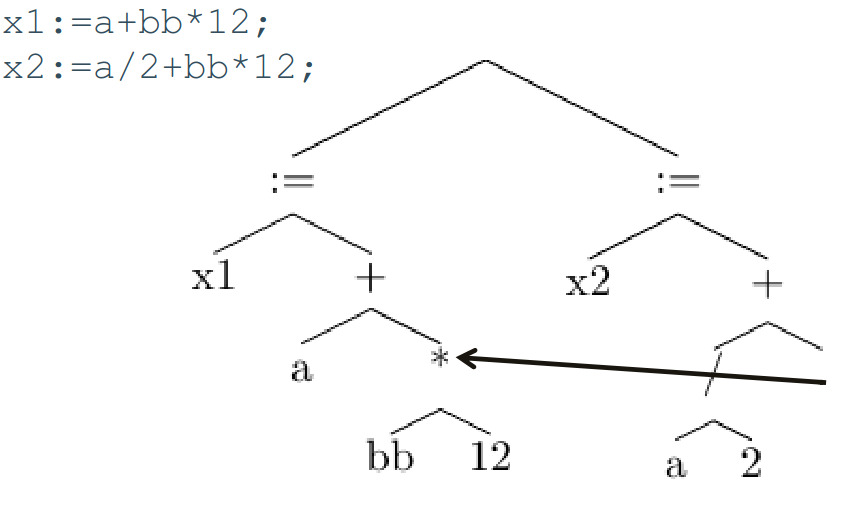
\includegraphics[width=1.00\textwidth]{ottimizzazione_codice}
		\end{figure}
	\end{itemize}
	La parte di analisi di un compilatore si occupa quindi di \textbf{verificare la correttezza lessicale, sintattica e semantica di un programma} e:
	\begin{itemize}
		\item viene svolta in fase di compilazione;
		\item verifica che:
		\begin{itemize}
			\item I simboli utilizzati siano legali, cioè appartengano all'alfabeto (analisi lessicale);
			\item Le regole grammaticali siano rispettate (analisi sintattica);
			\item I vincoli imposti dal contesto siano rispettati (analisi semantica).
		\end{itemize}
	\end{itemize}
	Ad esempio: \\
	\begin{lstlisting}
		var A: integer;
		...
		if A then ... ERRORE
	\end{lstlisting}
	\section{Generatore di codice}
	L'output dell'analizzatore semantico è passato al generatore di codice che trasla la forma intermedia in linguaggio assembler o macchina. \\
	Prima della generazione del codice oggetto ci sono delle fasi di preparazione:
	\begin{itemize}
		\item Allocazione della memoria: può essere allocata statica oppure è uno stack o heap la cui dimensione cambia durante l'esecuzione;
		\item Allocazione dei registri: poichè l'accesso ai registri è più rapido dell'accesso alle locazioni di memori,a, i valori cui si accede più spesso andrebbero mantenuti nei registri.
	\end{itemize}
	Ad esempio:
	\begin{lstlisting}
		x1 := a + bb * 12;
		x2 := a / 2 + bb * 12;
	\end{lstlisting}
	Potremmo pensare di allocare l'espressione bb * 12 al registro 1, ed una copia del valore di $a$ nel registro 2 assieme al valore $a/2$.\\
	Le variabili si potrebbero allocare sullo stack con $a$ al top, e poi, nell'ordine, bb, x1, x2. Il registro $S$ punto al top dello stack. \\
	Segue poi la vera e propria generazione del codice. \\
	Ad esempio: \\
	(+, A, B, T1) \\ (+, C, D, T2) \\ (*, T1, T2, T3) \\
	Si possono produrre quindi le seguenti istruzioni assembler:
	\begin{tabular}{c c}
		LOADA & A \\
		LOADB & B \\
		STOREA & T1 \\
		LOADA & C \\
		LOADB & D \\
		STOREA & T2 \\
		LOADA & T1 \\
		LOADB & T2 \\
		MULT & \\
		STOREA & T3
	\end{tabular}
	\textbf{Nota}:
	\begin{itemize}
		\item (S), 1(S), 2(S), ecc.: accede al contenuto del top dello stack, ad una posizione successiva, due posizioni successive, ecc. 
		\item @A: accede alla locazione il cui valore è puntato da A, ovvero non prende il contenuto della cella A ma ne prende l'indirizzo (indirizzamento indiretto)
	\end{itemize}
	Ad esempio:
	\begin{lstlisting}
		x1 := a + bb * 12;
		x2 := a / 2 + bb * 12;
	\end{lstlisting}
	Possiamo generare per una macchina di nostra invenzione il seguente codice:
	\begin{figure}[H]
		\centering
		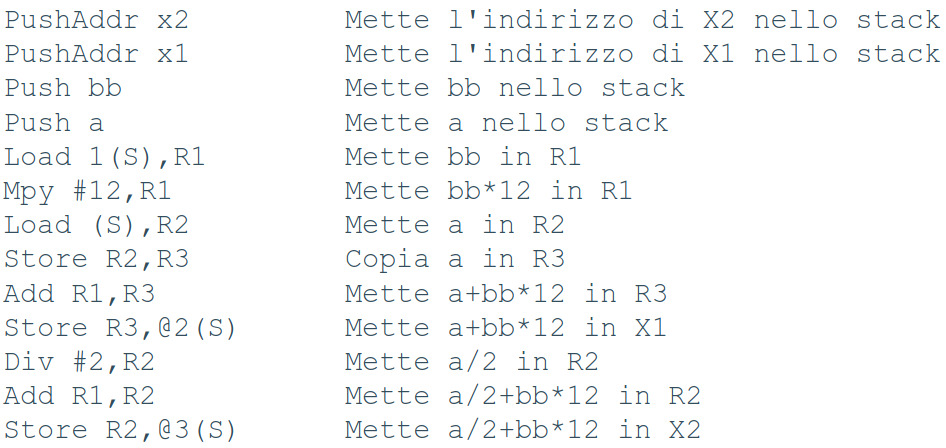
\includegraphics[width=1.00\textwidth]{generazione_codice}
	\end{figure}
	\section{Ottimizzatore di codice}
	L'output del generatore di codice è passato in input all'ottimizzatore di codice, presente nei compilatori più sofisticati. \\
	Ci sono due tipi di ottimizzazione:
	\begin{itemize}
		\item \textbf{Ottimizzazioni indipendenti dalla macchina:} ad esempio la rimozione di istruzioni invarianti all'interno di un loop, fuori dal loop, ecc.
		\item \textbf{ottimizzazioni dipendenti dalla macchina}: ad esempio ottimizzazione dell'uso dei registri.
	\end{itemize}
	Ad esempio:
	\begin{figure}[H]
		\centering
		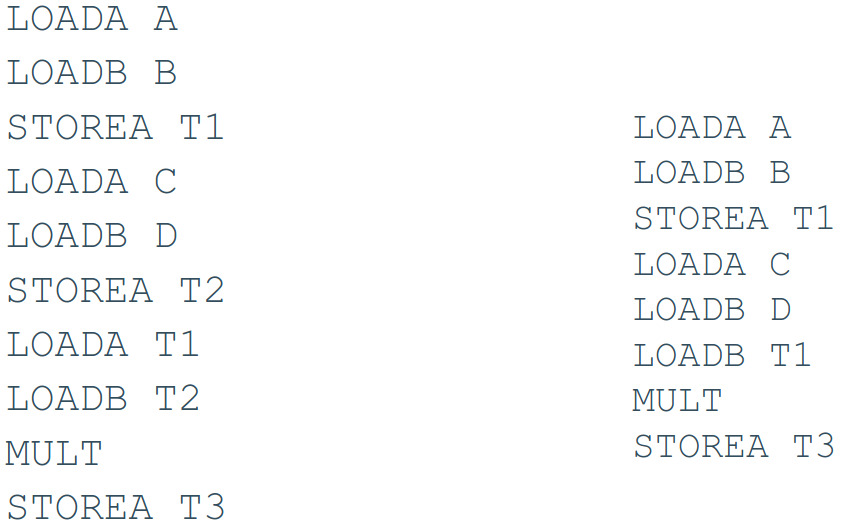
\includegraphics[width=1.00\textwidth]{ottimizzatore_del_codice}
	\end{figure}
	\section{Passi di un compilatore}
	Scanner e parser possono essere eseguiti in sequenza uno dopo l'altro, producendo prima tutti i token e poi l'analisi sintattica, oppure lo scanner è chiamata dal parser ogni volta che necessita un nuovo token. \\
	Nel primo caso lo scanner ha esaminato l'intero programma sorgente prima di passare il controllo al parser e quindi ha compiuto un intero passo separato. \\
	A volte il parser, l'analizzatore semantico ed il generatore di codice sono combinati in un singolo passo. \\
	Alcuni compilatori sono solo ad un passo, altri anche fino a 30. \\
	Altri aspetti importanti della compilazione sono:
	\begin{itemize}
		\item Error Detection e Recovery;
		\item Le Tabelle dei Simboli prodotte dai vari moduli;
		\item La Gestione della Memoria implicata da alcuni costrutti del linguaggio di alto livello.
	\end{itemize}
	Le fasi di più semplice progettazione, con un apparato formale ben sviluppato e quindi facilmente automatizzabili sono scanner e parser, mentre maggiore difficoltà si trova nella progettazione di analizzatori semantici, generatori ed ottimizzatori di codice. 
	\section{Linking e Caricamento}
	Il programma oggetto prodotto dal compilatore contiene una serie di riferimenti esterni come riferimenti a programmi di libreria, funzioni, ecc. \\
	I riferimenti esterni vengono risolti dal \textbf{linker}. \\
	Il programma è rilocabile: può essere allocato in diverse zone di memoria cambiando indirizzo $ind$,  (\textbf{indirizzamento relativo}). \\
	La fase di caricamento è compiuta dal \textbf{loader} che assegna un valore numeri all'indirizzo $ind$, trasformando gli indirizzi relativi in assoluti. \\
	Ad esempio: 
	\begin{figure}[H]
		\centering
		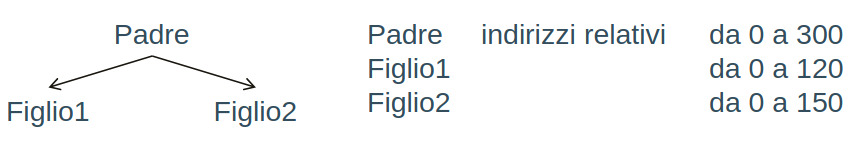
\includegraphics[width=1.00\textwidth]{linking}
	\end{figure}
	Il linker riceve in ingresso questi tre moduli e genera un unico modulo con riferimento ad indirizzi contigui a parte da un indirizzo simbolico $ind$. \\
	Ogni riferimento a moduli esterni viene sostituito con l'indirizzo così calcolato. \\
	Ad esempio:
	\begin{figure}[H]
		\centering
		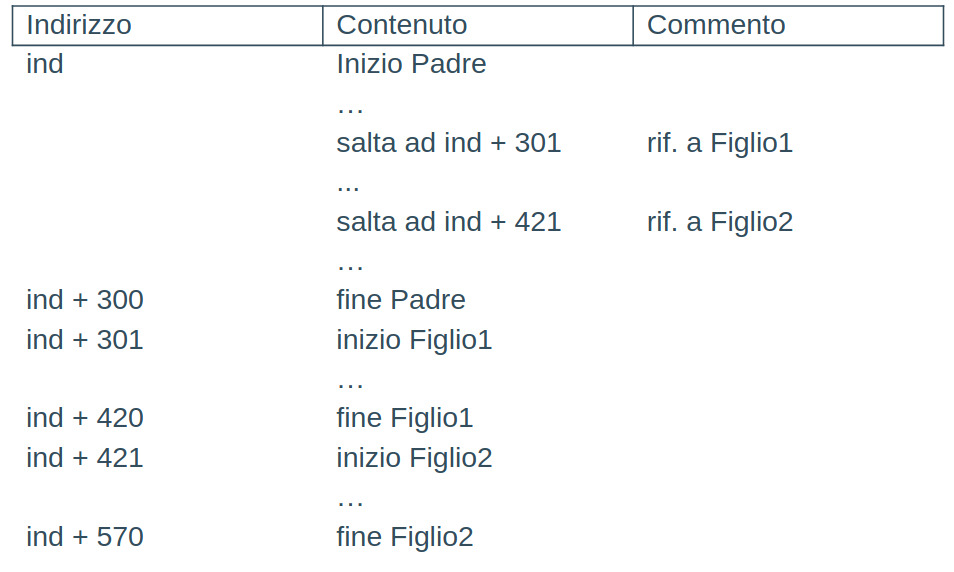
\includegraphics[width=1.00\textwidth]{linking_caricamento}
	\end{figure}
	\chapter{Analizzatore lessicale}
	Lo \textbf{scanner} rappresenta un'interfaccia fra il programma sorgente e l'analizzatore sintattico o parser. \\
	Lo scanner, attraverso un esame carattere per carattere dell'ingresso, separa il programma sorgente in parti chiamate token che rappresentano i nomi delle variabili, operatori, label, ecc. \\
	Il parser genera un albero sintattico le cui foglie sono i simboli terminali della grammatica, ovvero i token che lo scanner ha estratto dal programma sorgente e passato al parser. \\
	Il parser potrebbe fare direttamente anche l'analisi lessicale, ma non è conveniente in quanto la grammatica per i token è una grammatica di tipo 3, più semplice quindi di quella che tratta il parser. \\
	Lo scanner può interagire con il parser in due modi differenti:
	\begin{itemize}
		\item lavorare in un passo separato, producendo i token in una grossa tabella in memoria di massa;
		\item interagire direttamente con il parser che chiama lo scanner quando è necessario il prossimo token nell'analisi sintattica e questo approccio è preferibile.
	\end{itemize}
	Lo scanner suddivide il programma sorgente in \textit{token}. \\
	Il tipo di token è rappresentato con un numero intero, ad esempio le variabili con il numero 1, le costanti con il 2, ecc. \\
	Il token, che è una stringa di caratteri, è memorizzato in una tabella. \\
	I valori delle costanti sono memorizzati in una \textbf{costant table}, mentre i nomi delle variabili in una \textbf{symbol table}. \\
	\begin{figure}[H]
		\centering
		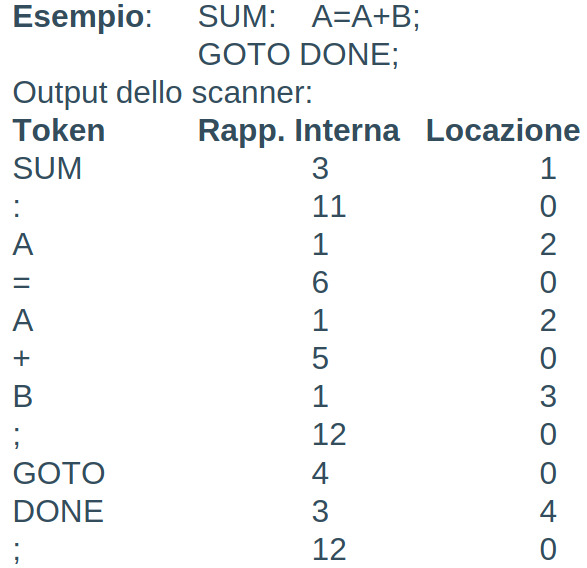
\includegraphics[width=1.00\textwidth]{lexer}
	\end{figure}
	Si noti che gli spazi bianchi sono stati ignorati dallo scanner. \\
	\subsection{Il progetto di uno scanner e la sua realizzazione}
	I compiti di uno scanner sono:
	\begin{itemize}
		\item Eliminare spazi bianchi, commenti, ecc;
		\item Isolare il prossimo token dalla sequenza di caratteri in input;
		\item Isolare identificatori e parole-chiave;
		\item Generare la symbol table;
		\item I token possono essere descritti in diversi modi. Spesso si utilizzano le \textbf{grammatiche regolari}.
	\end{itemize}
	Ad esempio, una grammatica per generare una grammatica regolare è la seguente:
	\begin{lstlisting}
		< uint > ::= 0 | 1 | 2 | 3 | 4 | 5 | 6 | 7 | 8 | 9 | 
					 0 < uint > | 
					 1 < uint > |
					 ... 
					 9 < uint > 
	\end{lstlisting}
	Un altro modo per descrivere i token è in modo riconoscitivo piuttosto che generativo mediante \textbf{automi a stati finiti}.\\
	\subsection{Esempio di scanner}
	Generare un diagramma a stati finiti per un linguaggio che consiste dei token: $<, \leq, =, \geq, <>, (, ), +, -, *, /, :=, ;$, \textbf{identificatori}, \textbf{parole chiave}, \textbf{costanti} e \textbf{stringhe} (fra apici). \\
	Commenti $(/* \ e\ * /)$ o spazi bianchi sono ignorati. \\
	\paragraph{Algoritmo} \quad \\
	Implementa lo scanner specificato dall'automa a stati finiti illustrato di seguito. \\
	\textbf{Procedure}:
	\begin{itemize}
		\item SCAN(PROGRAM, LOOKAHEAD, CHAR, TOKEN, POS) \\
		Data la stringa sorgente PROGRAM, questo algoritmo restituisce il numero di rappresentazione interna del TOKEN successivo nella stringa. \\
		Se TOKEN rappresenta un identificatore, stringa o costante, la procedura restituisce anche la sua posizione numerica nella tabella POS. \\
		CHAR rappresenta il carattere corrente su cui si sta facendo l'analisi lessicale. \\
		LOOKAHEAD è una variabile logica che ci dice se il simbolo in CHAR è stato usato nella chiamata precedente a SCAN. Un valore "false" denota che non è stato ancora controllato. \\
		L' algoritmo utilizza le seguenti funzioni: 
		\begin{itemize}
			\item GET\_CHAR(PROGRAM) che restituisce il prossimo carattere del programma sorgente;
			\item INSERT(STRING, type) che inserisce un dato token STRING (se necessario) ed il suo tipo nella tabella dei simboli;
			\item KEYWORD(STRING) che restituisce il numero di rappresentazione interna del suo argomento se è una keyword, 0 altrimenti. STRING contiene il token corrente. 
		\end{itemize}
	\end{itemize}
	Le variabili DIVISION, LEQ, NEQ, LTN, GEQ, GTN, EQ, LEFT, RIGHT, ADDITION, SUBTRACTION, MULTIPLICATION, ASSIGNMENT, SEMICOLON, LITERAL, IDENTIFIER e COSTANT contengono i numeri interni di rappresentazione dei token elencati precedentemente.
	\begin{figure}[H]
		\centering
		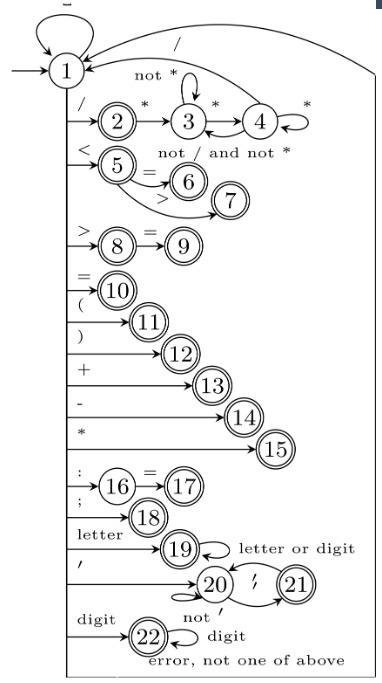
\includegraphics[width=0.75\textwidth]{algoritmo_es_scanner}
	\end{figure}
	La spiegazione dell'automa in maniera dettagliata è descritta nelle slide. \\
	\textbf{Algoritmo:}
	\begin{enumerate}
		\item \begin{lstlisting}
				[ Initialize. ]
				POS <- 0
			\end{lstlisting}
		\item \begin{lstlisting}
			[ Get first character ]
			if not LOOKAHEAD
			then CHAR <- GET_CHAR(PROGRAM) 
			LOOKAHEAD <- false
		\end{lstlisting}
		\item\begin{lstlisting}
				[ Loop until a token is found ]
				Repeat step 4 while true
			\end{lstlisting}
		\item
		\begin{lstlisting}
			[ Case statement to determine next token ]
			Select by (CHAR)
			Case '':
				CHAR <- GET_CHAR(PROGRAM)
			Case '/':
				CHAR <- GET_CHAR(PROGRAM)
				if CHAR = '*'
				then Repeat while true
					CHAR <- GET_CHAR(PROGRAM)
					if CHAR = '*'
					then Repeat while CHAR = '*'
							CHAR <- GET_CHAR(PROGRAM)
						if CHAR = '/'
						then CHAR <- GET_CHAR(PROGRAM)
							Exit loop
					else LOOKAHEAD <- true
						TOKEN <- DIVISION
						Return
			Case '<':
				CHAR <- GET_CHAR(PROGRAM)
				if CHAR = '='
				then TOKEN <- LEQ
				else if CHAR = '>'
					then TOKEN <- NEQ
					else LOOKAHEAD <- true
				TOKEN <- LTN
				Return
			Case '>':
				CHAR <- GET_CHAR(PROGRAM)
				if CHAR = '='
				then TOKEN <- GEQ
				else LOOKAHEAD <- true
				TOKEN <- GTN
				Return
			Case '=':
				TOKEN <- EQ
				Return
			Case '(':
				TOKEN <- LEFT
				Return
			Case ')':
				TOKEN <- RIGHT
				Return
			Case '+':
				TOKEN <- ADDITION
				Return
			Case '-':
				TOKEN <- SUBTRACTION
				Return
			CASE '*':
				TOKEN <- MULTIPLICATION
				Return
			CASE ':':
				CHAR <- GET_CHAR(PROGRAM)
				if CHAR = '='	
				then TOKEN <- ASSIGNMENT
					Return 
				else 
					CHAR <- GET_CHAR(PROGRAM)
					Write('Unknown token <<:>>', CHAR, 'IN SOURCE STRING')
			Case ';':
				TOKEN <- SEMICOLON
				Return
			Case '''':
				STRING <- ''
				Repeat while true
					CHAR <- GET_CHAR(PROGRAM)
					if CHAR = ''''
					then CHAR <- GET_CHAR(PROGRAM)
						if CHAR != ''''
						then LOOKAHEAD <- true
							POS <- INSERT(STRING, LITERAL)
							TOKEN <- LITERAL
							Return
					STRING <- STRING * CHAR
			Default:
				if CHAR >= 'A' and CHAR <= 'Z'
				then STRING <- CHAR
					CHAR <- GET_CHAR(PROGRAM)
					Repeat while (CHAR >= 'A' AND CHAR <= 'Z')
					or (CHAR >= '0' AND CHAR <= '9')
						STRING <- STRING * CHAR
						CHAR <- GET_CHAR(PROGRAM)
					LOOKAHEAD <- true
				if KEYWORD(STRING) > 0
				then TOKEN <- KEYWORD(STRING)
					Return
				POS <- INSERT(STRING, IDENTIFIER)
				TOKEN <- IDENTIFIER
				Return
				if CHAR >= '0' and CHAR <= '9'
				then STRING <- CHAR
					CHAR <- GET_CHAR(PROGRAM)
					Repeat CHAR >= '0' and CHAR <= '9'
						STRING <- STRING * CHAR
						CHAR <- GET_CHAR(PROGRAM)
					LOOKAHEAD <- true
					POS <- INSERT(STRING, COSTANT)
					TOKEN <- CONSTANT
					Return
				Write('ERROR UNKWOWN CHARACTER', CHAR, 'IN SOURCE STRING')
				CHAR <- GET_CHAR(PROGRAM)
		\end{lstlisting}
	\end{enumerate}
	\textbf{Osservazione:} In alcuni linguaggi non è possibile determinare sempre cos'è un token nel momento in cui è stato letto completamente. \\
	(Vedere esempio di Fortran dalle slide). \\
	\section{Linguaggi regolari e scanner}
	I linguaggi regolari vengono riconosciuti in modo efficiente attraverso automi a stati finiti. Tuttavia, sono linguaggi abbastanza limitati e con le loro grammatiche non si possono descrivere anche semplici costrutti dei linguaggi di programmazione. \\
	L'utilizzo dei linguaggi regolari e delle grammatiche lineari destre è perciò limitato alla costruzione ( e riconoscimento ) dei simboli base usati in un programma (quello che si indica generalmente come lessico), ad esempio gli identificatori. \\
	Il riconoscimento di tali simboli base è la prima fase durante la compilazione di un programma e prende il nome di analisi lessicale. \\
	Una volta terminata l'analisi lessicale sono stati individuati, ad esempio, le costanti, le variabili, ecc. utilizzate nel programma e costruita quella che si chiama tabella dei simboli. \\
	L'analisi del programma prosegue poi con tecniche più complesse, analisi sintattica e analisi semantica. \\
	I linguaggi regolari e le espressioni regolari possono essere usati per rappresentare scanner che sono implementati come automi a stati finiti. \\
	Poichè realizzare un automa a stati finiti è banale sono stati progettati programmi in grado di generare automaticamente degli scanner usando un metodo formale per specificare l'automa a stati finiti. \\
	\section{Lex}
	Un noto generatore di scanner è \textbf{Lex} (1975) che utilizza espressioni regolari per specificare lo scanner. \\
	Utilizzando espressioni regolari ed associati segmenti di codice chiamati azioni, Lex genera una tabella delle transizioni e un programma che interpreta tale tabella. \\
	L'azione è eseguita quando si riconosce un token generato dall'espressione regolare. L'output di Lex è quindi un programma che simula un automa a stati finiti ed esegue le funzioni addizionali associati con le azioni. \\
	Lo scanner generato da Lex può essere usato in congiunzione con un parser (YACC) per eseguire sia l'analisi lessicale che sintattica.	
	\chapter{Tabella dei simboli}
	Le tabelle dei simboli servono a due scopi:
	\begin{enumerate}
		\item controllano la correttezza semantica ( la parte dal contesto della grammatica );
		\item aiutano nella generazione del codice.
	\end{enumerate}
	Tutte queste attività si ottengono mediante accesso alla tabella dei simboli per inserire o leggere alcuni attributi delle variabili del programma sorgente. \\
	Questi attributi sono: tipo, nome, dimensione, indirizzo e si determinano direttamente dalla dichiarazione o implicitamente dal contesto in cui le variabili compaiono. \\
	Discuteremo l'organizzazione della tabella dei simboli e la modalità per creare ed accedere simboli. La tabella dei simboli è inserita in memoria centrale e viene normalmente modificata dinamicamente. \\
	Ogni identificatore del programma sorgente richiede da parte del compilatore accessi alla tabella dei simboli. Questo spiega perchè l'accesso alla tabella dei simboli sia una delle parti più costose in tempo del processo di compilazione e si debba cercare di ottimizzare. \\
	Quindi è importante studiare metodi efficienti per l'accesso alla tabella dei simboli.
	\section{Strutture dati: tavole o tabelle}
	Una tavola o tabella è un tipo di dato astratto per rappresentare insiemi di coppie $<chiave, attributi>$. Ciascuna coppia rappresenta dati riferiti ad un'unica entità logica identificata in modo univoco dalla \textbf{chiave}. \\
	Un'esempio tipico è:
	\[
	Matricola, \quad Cognome, Nome, DataDiNascita, \dots
	\]
	\subsection{Operazioni tipiche sulle tavole}
	\begin{itemize}
		\item \textbf{Inserimento} di un elemento $<chiave, attributi>$: \\
		$inserisci:\ tavola \times chiave \times attributi \to tavola$
		\item \textbf{Cancellazione} di un elemento ( nota la chiave ) \\
		$cancella:\ tavola \times chiave \to tavola$
		\item \textbf{Verifica di appartenenza di un elemento}: \\
		$esiste:\ tavola \times chiave \to boolean$ 
		\item \textbf{Ricerca} di un elemento nella tavola: \\
		$ricerca:\ tavola \times chiave \to attributi$
	\end{itemize}
	L'operazione di ricerca è la più, soprattutto nelle tabelle dei simboli dei compilatori. Spesso la rappresentazione concreta viene scelta in modo da ottimizzare questa operazione. \\
	In Pascal, ciascun elemento della tavola rappresenta una \textbf{aggregazione} di dati che è un \textbf{record}. La chiave e ciascun attributo corrispondono ad un \textbf{campo del record}.
	\section{Quando costruire ed interagire con la tabella dei simboli}
	In un compilatore a molti passi, la tabella dei simboli viene creata durante l'analisi lessicale. \\
	Gli indici degli entries per le variabili nella TS formano parte della stringa di tokens prodotta dallo scanner. \\
	Nella figura seguente se $X$ e $Y$ occupano le posizione 1 e 2 nella TS si generano i tokens i1 e i2. \\
	Quando il parser produce l'albero sintattico, le foglie hanno dei riferimenti alla tabella dei simboli. \\
	L'analisi sintattica comunque non produce modifiche a TS, solo durante l'analisi semantica e la generazione di codice si possono assegnare valori agli attributi della variabile in TS. 
	\begin{figure}[H]
		\centering
		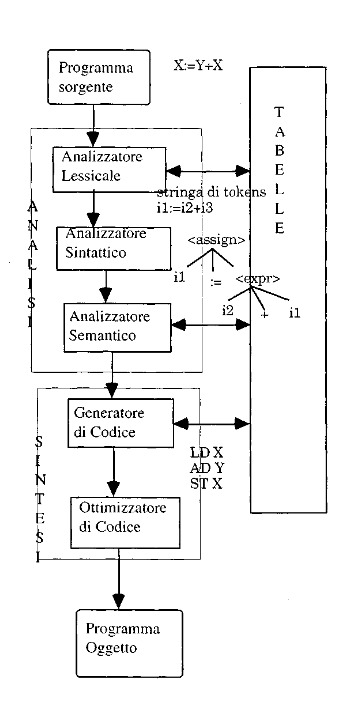
\includegraphics[width=0.50\textwidth]{TS_compilatori}
	\end{figure}
	\section{Contenuti della TS}
	Una TS è costituita da una serie di righe ognuna delle quali contiene una lista di valori di attributi associati con una particolare variabile. \\
	Gli attributi dipendono dal linguaggio di programmazione che si compila, ad esempio se non ha i tipi non comparirà tale attributo. \\
	\begin{figure}[H]
		\centering
		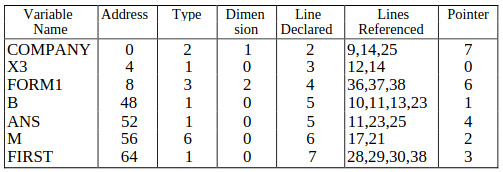
\includegraphics[width=0.5\textwidth]{TS_esempio}
	\end{figure}
	Si possono considerare i seguenti attributi:
	\begin{enumerate}
		\item Nome della variabile;
		\item Indirizzo nel codice oggetto;
		\item Tipo;
		\item Numero dei parametri di una procedura o dimensione della variabile;
		\item Linea sorgente in cui la variabile;
		\item Linee sorgente in cui la variabile è referenziata;
		\item Puntatori per listarli in ordine alfabetico.
	\end{enumerate}
	Commentiamo tali attributi:
	\begin{enumerate}
		\item Nome della variabile. Un problema può essere la dimensione della stringa che compone il nome. È inserito dallo scanner.
		\item Indirizzo nel codice oggetto. L'indirizzo indica la locazione relativa delle variabili a run-time. Questo è inserito nella TS quando una variabile è dichiarata o incontrata per la prima volta. È richiamato dalla tabella quando la variabile è referenziata nel codice per generare il codice oggetto corrispondente. \\
		Per un linguaggio senza allocazione dinamica di memoria, come il FORTRAN, gli indirizzi sono attribuiti in modo sequenziale da 1 a M dove M è la massima dimensione di memoria allocata per il programma. \\
		Per i linguaggi a blocchi, l'indirizzo è rappresentato da una coppia $<BL\ (block\ level), ON\ (occurence\ number)>$. A run-time ON rappresenta l'offset rispetto al blocco.
		\item Tipo. Il tipo può essere implicito come il FORTRAN, esplicito come il PASCAL o può non esistere come nel LISP o PROLOG. Il tipo della variabile è fondamentale per il controllo semantico. Ad esempio, $S * 3$ è scorretto se $S$ è dichiarato come una variabile di tipo stringa.
		\item Il tipo serve anche per sapere quanta memoria deve essere allocata per la variabile. Il tipo è inserito normalmente con una codifica, come un numero intero.
		\item Dimensione della variabile. La dimensione è importante per il controllo semantico. Se si tratta di un array ci dice le sue dimensioni e serve anche per calcolare l'indirizzo di un particolare elemento dell'array. In una procedura indichiamo il numero di parametri per procedere al controllo durante le chiamate. \\
		Negli esempi dati precedentemente, gli scalari sono considerati di dimensione 0, i vettori di 1, le matrici di 2, ecc.
		\item L'ultimo attributo, il Pointer, serve per costruire, ad esempio, una lista per ordine alfabetico della tabella dei simboli od una cross-reference (con riferimenti di dove è dichiarata e referenziata nel codice sorgente).
	\end{enumerate}
	\subsection{Operazioni sulla tabella dei simboli}
	Le operazioni più comuni sono l'\textbf{inserimento} e la \textbf{ricerca}. \\
	Se il linguaggio ha dichiarazioni esplicite di tutte le variabili allora l'inserimento avviene al momento della dichiarazione. \\
	Se la tabella dei simboli è ordinata, ad esempio, alfabeticamente mediante il nome della variabile si deve fare anche una ricerca nella tabella e quindi diventa un procedimento costoso. \\
	Se invece la tabella è disordinata l'inserimento è rapido. ma diventa poi più inefficiente la ricerca. \\
	Le operazioni di ricerca vengono svolte per ogni riferimento a variabili in istruzioni non di dichiarazione. \\
	L'accesso serve per il controllo semantico e la generazione di codice, nonchè la rilevazione di errori se le variabili non si trovano all'interno della tabella. \\
	Quando un linguaggio ha la possibilità di dichiarare variabili implicitamente allora le operazioni di inserimento e ricerca sono legate strettamente. \\
	Ogni riferimento ad una variabile genera una ricerca ed eventualmente un inserimento se non è già stata inserita in TS. \\
	\paragraph{Linguaggi a blocchi} \quad \\
	Per i linguaggi a blocchi sono necessarie due operazioni addizionali che chiamiamo \textbf{set} e \textbf{reset}. \\
	Set si invoca quando si entra in un blocco, reset quando si esce. \\
	Questo è necessario perchè in un linguaggio a blocchi, una variabile con lo stesso nome può essere dichiarata in punti diversi del programma ed assumere attributi diversi. \\
	In un linguaggio innestato è importante assicurare che per ogni istanza di un nome di variabile sia associato un unico entry nella TS. \\
	Quindi ad ogni inizio di un blocco l'operazione di set attribuisce una nuova sotto tabella per gli attributi delle variabili dichiarate nel nuovo blocco. \\
	Supponiamo che le sottotavole siano create attribuendole numeri interi crescenti. \\
	Se la ricerca comincia nella sottotavola N e poi procede fino alla sottotavola 1, la variabile che si trova è l'ultima che è si è inserita ed è eliminata ogni ambiguità. \\
	All'uscita del blocco, l'operazione di reset rimuove l'ultima sottotabella allocata. Le variabili di quel blocco, infatti, non possono più essere referenziate.
	\section{Organizzazione delle TS per linguaggi non a blocchi}
	Intendiamo linguaggi in cui ogni singola unità di compilazione è un modulo senza alcun sottomodulo. \\
	Tutte le variabili dichiarate nel modulo possono essere referenziate in ogni parte del modulo. 
	\subsection{TS non ordinate}
	Il modo più semplice di organizzare una tabella dei simboli è quello di aggiungere gli entries alla tabella nell'ordine in cui le variabili sono dichiarate. \\
	In questo modo per un inserimento non è richiesto nessun confronto, mentre una ricerca richiede, nel caso peggiore, il confronto con gli N elementi all'interno della tabella. \\
	Poichè ciò è inefficiente, questa organizzazione dovrebbe essere adottata solo la dimensione della TS è piccola, altrimenti si deve ricorrere ad altre organizzazioni.
	\paragraph{Rappresentazione in Pascal} \quad \\
	In memoria centrale, realizzata attraverso \textbf{array}.
	\begin{lstlisting}
		const N = 100;
		type  key = packed array[1..10] of char;
			  elem = record
			  	chiave: key;
			  	address: integer;
			  	typeel: integer;
			  	dimension: integer;
			  	lineD: integer;
			  	lineR: array[1..100] of integer;
			  	pointers: 0..N
			  	end;
			index = 1..N;
			Tavola = array[index] of elem;
		var T: Tavola;
	\end{lstlisting}
	È necessario porre un limite massimo alla dimensione della tavola, al massimo N elementi. \\
	Lo spazio di memoria occupato è fisso, indipendente dal numero di elementi della tavola. \\
	La ricerca è sequenziale ed esaustiva, il caso peggiore sono N confronti.
	\begin{lstlisting}
		procedure ricerca(var T: Tavola; k: key; var el: elem; var trovato: boolean);
		var i: 1..N;
		begin
			i := 1;
			trovato := false;
			while (i <= N) and (not trovato) do
				if T[i].chiave = k
				then begin
					 trovato := true;
					 el: T[i]
					 end
				else i := i + 1
		end;
	\end{lstlisting}
	\subsection{TS ordinate}
	La posizione dell'elemento nella TS è determinata dal nome della variabile, ordinamento lessicale. \\
	In questo caso un inserimento è sempre accompagnato ad una procedura di ricerca. \\
	L'inserimento può inoltre richiedere uno spostamento di altri elementi già inseriti nella tabella e questa è la maggiore fonte di inefficienza. \\
	L'\textbf{ottimizzazione della ricerca} si ottiene se gli elementi sono memorizzati in modo ordinato nella tavola. \\
	Deve esistere un ordinamento sul campo Chiave. Questo induce un ordinamento sugli elementi della Tavola come segue:
	\begin{lstlisting}
		el1 = < k1, Attr1 >
		el2 = < k2, Attr2 >
				el1 < el2		se e solo se k1 < k2 
	\end{lstlisting}
	La ricerca può arrestarsi appena si incontra un elemento con chiave maggiore di quella cercata, il caso medio è di $\frac{N}{2}$ confronti, nel caso peggiore sono $N$ confronti. \\
	Si complica l'operazione di inserimento di un nuovo elemento nella tavola ma occorre mantenerla ordinata. \\
	Un miglioramento ulteriore è la \textbf{ricerca binaria}. \\
	Si accede all'elemento mediano $< chiave, attr >$ della tavola. Se $chiave = k$, fine della ricerca. \\
	Altrimenti, se $k < chiave$ viene ripetuta la ricerca nella prime metà della tavola, se $k > chiave$ viene ripetuta la ricerca nella seconda metà della tavola. \\
	Ricerca binaria su tavola ordinata realizzata mediante array:
	\begin{figure}[H]
		\centering
		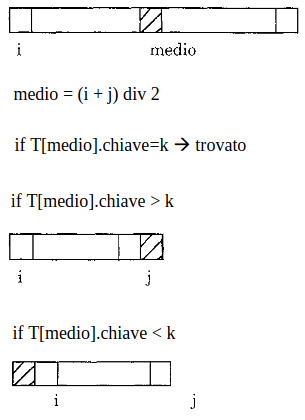
\includegraphics[width=0.5\textwidth]{ricerca_TS}
	\end{figure}
	Il procedimento si arresta quando: $i=j$
	\begin{lstlisting}
		procedura ricerca_bin(var T: Tavola; k: key; i,j:
		index; var el: elem; var trovato: boolean);
		var medio: 1..N;
		begin
			trovato := false;
			if (j > i) and ( not trovato ) then
				begin
				medio := (i + j) div 2;
				if T[medio].chiave = k
				then trovato := true
				else 
					if T[medio].chiave > k
					then
					ricerca_bin(T, k, i, pred(medio), el, trovato)
					else
					ricerca_bin(T, k, succ(medio), j, el , trovato)
				end
			else if T[i].chiave = k then trovato := true
		end;
	\end{lstlisting}
	Ad ogni passo si eliminano dalla ricerca metà degli elementi della tavola corrente. Nel caso peggiore si eseguono $\log_2{N}$ confronti.
	\subsection{Tavole: rappresentazione collegata e ad albero}
	Il tempo per inserire un elemento in una TS ordinata si può ridurre utilizzando una struttura collegata o ad albero. \\
	Nel caso di \textbf{rappresentazione collegata} di una tavola, si utilizza una lista semplice:
	\begin{lstlisting}
		const N = 100;
		type  key = packed array[1..10] of char;
			  ptr_tavola=^elem;
			  elem=record
			  	chiave:key;
			  	address:integer;
			  	typeel:integer;
			  	dimension=integer;
			  	lineD:integer;
			  	lineR:array[1.100] of integer;
			  	next: ptr_tavola
			  end;
			index = 1..N;
			Tavola = array [index] of elem;
		var T: Tavola;
	\end{lstlisting}
	Nella rappresentazione collegata, l'idea fondamentale è quella di memorizzare gli elementi associando a ciascuno una particolare informazione (\textbf{ riferimento }) che permetta di individuare la locazione in cui è inserito l'elemento successivo. \\
	La sequenzialità degli elementi della lista non è rappresentata mediante l'adiacenza delle locazioni di memoria in cui sono memorizzati. \\
	Segue una notazione grafica per la rappresentazione collegata: elementi della lista come nodi e riferimenti come archi. \\
	Lista: [5, 8, 21]
	\begin{figure}[H]
		\centering
		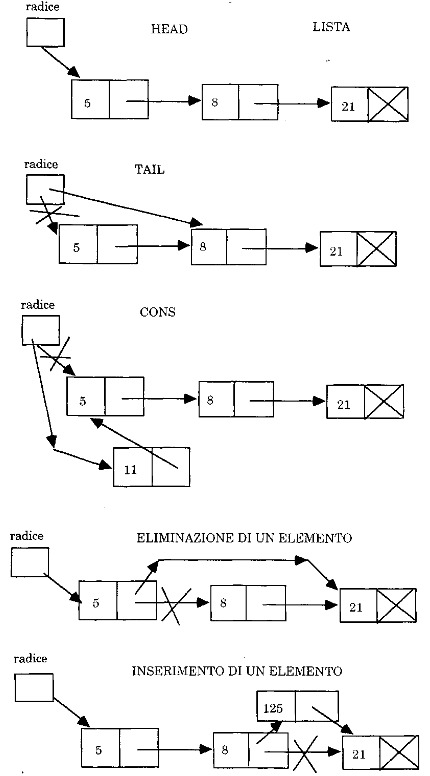
\includegraphics[width=0.40\textwidth]{rappresentazione_collegata_TS}
	\end{figure}
	Non c'è un limite massimo alla dimensione della tavola. \\
	Lo spazio di memoria occupato dipende solo dal numeri di elementi della tavola. Se la lista è ordinata sulla chiave, si può applicare la ricerca ordinata ( ci si arresta al primo elemento con chiave $>=$ ).
	\subsection{TS strutturate ad albero}
	Un albero ordinato in cui ogni nodo ha al massimo due figli \textbf{(figlio destro e figlio sinistro)}. \\
	La \textbf{definizione induttiva} è la seguente: Un albero binario è un grafo orientato aciclico che o è vuoto (cioè ha un insieme vuoto di nodi), oppure è formato da un nodo radice e da due sotto-alberi binari, sinistro e destro. \\
	La rappresentazione più efficiente, direttamente attraverso \textbf{record} e \textbf{pointer} in Pascal:
	\begin{figure}[H]
		\centering
		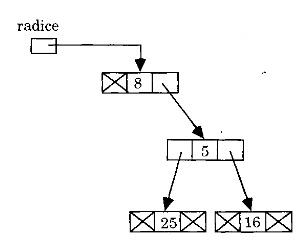
\includegraphics[width=0.4\textwidth]{TS_bin_tree}
	\end{figure}
	Ogni record \textbf{(nodo)} ha tre campi: uno per l'informazione associata al nodo, uno per il puntatore al sottoalbero sinistro ed uno per il puntatore al sottoalbero destro. \\
	\begin{lstlisting}
		type tree = ^node;
			 node = record
			 			value: Element_type;
			 			left, right: tree
			 		end;
	\end{lstlisting}
	I \textbf{vantaggi} di questo approccio è che non è necessario che l'albero sia completo; si ha un'occupazione di memoria efficiente e operare modifiche è agevole.
	Ad esempio:
	\begin{figure}[H]
		\centering
		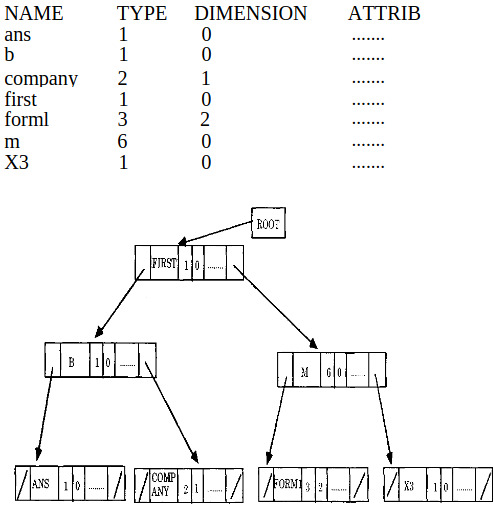
\includegraphics[width=0.5\textwidth]{es_TS_binari}
	\end{figure}
	\subsection{Algoritmi di visita per alberi binari}
	Consentono di analizzare tutti i nodi dell'albero in un determinato ordine.
	\begin{figure}[H]
		\centering
		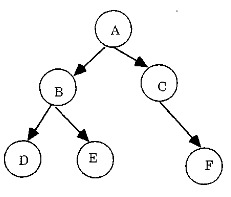
\includegraphics[width=0.5\textwidth]{es_albero_binario}
	\end{figure}
	\paragraph{Preordine o ordine anticipato} \quad \\
	Analizza radice, albero sinistro, albero destro.
	\begin{lstlisting}
		visita in preordine(T):
			se test-vuoto(T) = false
			allora esegui
				analizza radice(T)
				visita in preordine(sinistro(T))
				visita in preordine(destro(T))
			fine;
	\end{lstlisting}
	A B D E C F
	\paragraph{Postordine o ordine ritardato} \quad \\
	Analizza albero sinistro, albero destro radice.
	\begin{lstlisting}
		visita in postordine(T):
			se test-vuoto(T) = false
			allora esegui
				visita in postordine(sinistro(T))
				visita in postordine(destro(T))
				analizza radice(T)
			fine;
	\end{lstlisting}
	D E B F C A
	\paragraph{Simmetrica} \quad \\
	Analizza albero sinistro, radice, albero destro. 
	\begin{lstlisting}
		visita simmetrica(T):
			se test-vuoto(T)=false
			allora esegui
				visita simmetrica(sinistro(T))
				analizza radice(T)
				visita simmetrica(destro(T))
			fine;
	\end{lstlisting}
	D B E A C F
	\subsection{Alberi binari di ricerca}
	Gli alberi binari di ricerca sono alberi binari ordinati utilizzati per memorizzare grosse quantità di dati su cui si esegue spesso un'operazione di ricerca di un dato. \\
	In un albero binario di ricerca, ogni nodo N ha la seguente proprietà:
	\begin{itemize}
		\item tutti i nodi del sottoalbero sinistro di N hanno un valore minore o uguale a quello di N
		\item tutti i nodi del sottoalbero destro di N hanno un valore maggiore di quello di N
	\end{itemize}
	\begin{figure}[H]
		\centering
		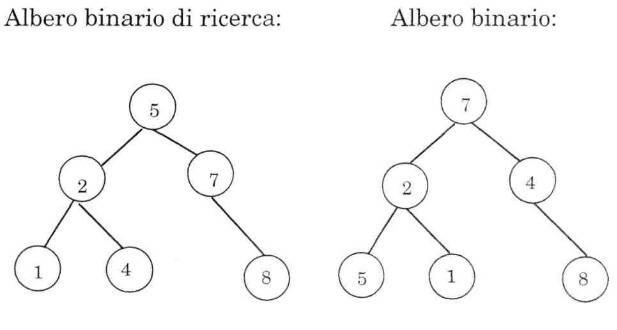
\includegraphics[width=0.6\textwidth]{btree_ricerca}
	\end{figure}
	\paragraph{Ricerca binaria in un albero binario di ricerca} \quad \\
	\begin{lstlisting}
		function alb_ric (e: Element_type; t: tree): boolean;
		begin 
		if empty(t)
		then alb_ric := false
		else 
			begin
			if isequal (e, root(t))
			then alb_ric := true
			else 
				if isless(e, root(t))
				then alb_ric := alb_ric(e, left(t))
				else alb_ric := alb_ric(e, right(t))
		end;
	\end{lstlisting}
	Il numero di confronti è, nel caso peggiore, proporzionale alla profondità dell'albero. Ad ogni passo si dimezza il problema, eliminando metà dei nodi. \\
	Inserimenti e cancellazioni devono essere fatte in modo da mantenere l'albero bilanciato. \\
	\paragraph{Alberi binari di ricerca: inserzione con bilanciamento} \quad \\
	Un nodo \textbf{perfettamente bilanciato} si ha quando l'altezza dei suoi due sottoalberi è la stessa. \\
	Un nodo \textbf{bilanciato a sinistra} si ha quando: $height(left(n)) = height(right(n)) + 1$. \\
	Un nodo \textbf{bilanciato a destra} si ha quando: $height(left(n)) = height(right(n)) - 1$ \\
	Un albero è bilanciato in altezza quando l'altezza del sottoalbero sinistro e destro di ogni nodo differisce al più di 1.
	\subsection{TS: rappresentazione a funzione di accesso}
	Usando questa rappresentazione, l'\textbf{obiettivo} è permettere il recupero con \textit{pochi accessi} di una registrazione nota la sua chiave. \\
	L'\textbf{idea base} è quella di definire una qualche forma di \textit{corrispondenza} fra i valori delle chiavi e le posizioni delle registrazioni nell'archivio in modo da rintracciare velocemente la registrazione richiesta. \\
	Ogni elemento è memorizzato in una posizione che dipende dal valore della chiave.
	\begin{figure}[H]
		\centering
		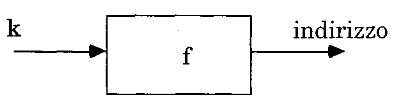
\includegraphics[width=0.4\textwidth]{hash}
	\end{figure}
	Ad esempio:
	\begin{lstlisting}
		< key > ::= < lettera > { < lettera > }^2
	\end{lstlisting}
	Quindi esistono 26 chiavi di lunghezza 1, $26^2$ chiavi di lunghezza 2 e $26^3$ chiavi di lunghezza 3. Le possibili chiavi sono: $26 + 676 + 17576 = 18278$ \\
	\begin{figure}[H]
		\centering
		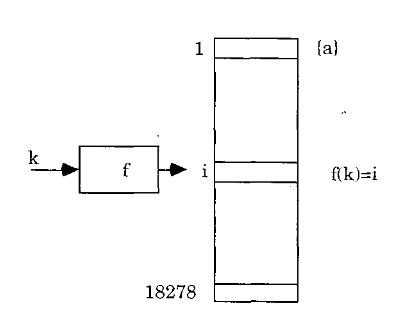
\includegraphics[width=0.5\textwidth]{hash_biunivoca}
	\end{figure}
	\paragraph{Funzione di accesso biunivoca} \quad \\
	La funzione di accesso biunivoca data la chiave $k$ restituisce il numero $i$ corrispondente a $k$. \\
	Quindi occorre una locazione di memoria per ciascuna possibile chiave. \\
	L'\textbf{accesso} è molto efficiente: data la chiave $k$, l'elemento ricercato è all'indirizzo $ind=f(k)$ nello spazio di memoria riservato alla tavola. \\
	Anche l'\textbf{inserimento} e la \textbf{cancellazione} sono realizzati in modo efficiente. \\
	L'utilizzo di una funzione di accesso biunivoca è possibile in pratica solo se il numero di elementi della tavola è circa uguale al numero di chiavi possibili. \\
	In alternativa, la funzione può calcolare lo stesso indirizzo per chiavi distinta e quindi si possono verificare delle \textbf{collisioni}, che si verificano quando $f(k_1) = f(k_2)$. \\
	In questo caso occorre:
	\begin{enumerate}
		\item scegliere una funzione di accesso che riduca il più possibile le collisioni;
		\item in caso di collisione, determinare un metodo di scansione della tavola ( per ricerca o inserimento ).
	\end{enumerate}
	\paragraph{Tabelle Hash} \quad \\
	Utilizzando le \textbf{funzioni hash} (tritare, mescolare), l'indirizzo calcolato dipende da tutta la chiave, eventualmente spezzata in parti "rimescolate". \\
	Ad esempio, chiave di 15 caratteri. Sia K la sua rappresentazione binaria: si calcola il resto della divisione di K per il massimo numero di elementi N previsto per la tavola. \\
	\textbf{Esempio:} \\
	Chiave: stringa di 3 lettere al massimo. Ogni chiave è associata ad un numero intero. Un intero può essere associato a più chiavi. \\
	Le chiavi sono partizionate in \textbf{classi di equivalenza}. \\
	\begin{lstlisting}
		type key: string[3];
		function hash (k: key): integer;
		var first: char;
		begin
			first := k[1];
			hash := (ord(first) - ord('a')) * length(k)
		end;
	\end{lstlisting}
	Valore min: \quad first = 'a' \quad length(k)=... $\to 0$ \\
	Valore max: \quad first = 'z' \quad length(k)=3 $\to 75$ \\
	Classi di equivalenza: chiavi di ugual lunghezza che iniziano con la stessa lettera. \\
	Le chiavi di una stessa classe di equivalenza \textbf{collidono}. \\
	\paragraph{Collisioni} \quad \\
	La funzione hash si dice perfetta se e solo se non produce collisioni. \\
	Il problema è che evitare collisioni non è facile. \\
	Tuttavia, l'overflow può essere evitato quando si riesce a stabilire una \textit{corrispondenza biunivoca} fra l'insieme delle possibili chiavi e l'insieme delle posizioni disponibili nell'area di memorizzazione. \\
	In generale, però, le chiavi possibili sono molto più di quelle realmente usate, e ciò rende questo approccio impossibile da adottare perchè drammaticamente inefficiente. \\
	Per questo si definisce il concetto di \textbf{densità delle chiavi attive}. \\
	Detto N il numero di registrazioni da archiviare e M la cardinalità dell'insieme delle chiavi, la densità delle chiavi attive è data dal rapporto $\dfrac{M}{N}$ \\
	\paragraph{Gestione delle collisioni} \quad \\
	\textbf{Metodi di scansione}, nel caso si verifichino collisioni:
	\textbf{Scansione lineare:} se $f(k_1) = f(k_2)$ si passa a considerare per $k_2$ l'indirizzo $i + h$, h prefissato, poi $i + 2*h$, $i + 3*h$, $\dots$. \\
	In alternativa, \textbf{scansione con aree di trabocco}: Area di trabocco con rappresentazione collegata (lista): 
	\begin{figure}[H]
		\centering
		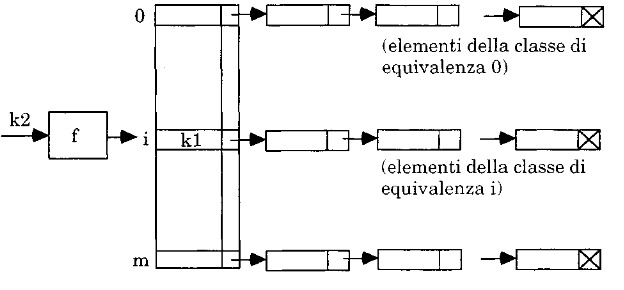
\includegraphics[width=0.6\textwidth]{area_di_trabocco}
	\end{figure}
	Altri metodi: albero, tabelle Hash. Può esserci anche un'unica area di trabocco per tutta la tavola. \\
	Una buona \textbf{funzione hash} deve assicurare:
	\begin{itemize}
		\item una distribuzione \textit{uniforme} delle chiavi nello spazio degli indirizzi
		\item una distribuzione \textit{casuale} delle chiavi, cioè valori vicini di chiave non devono finire in indirizzi vicini.
	\end{itemize}
	Alcune funzioni hash spesso usate sono:
	\begin{enumerate}
		\item metodo del modulo:
		\[
		H(k) = k \mod R
		\]
		con R = massimo numero primo minore o uguale a P
		\item metodo della somma:
		\[
		H(k) = (p1 + p2 + \dots + pS) mod 10^h
		\]
		dove $p1\dots pS$ sono pezzi della chiave k stessa, che viene suddivisa in parti fatte da un egual numero h di caratteri, pari all'ampiezza dell'indirizzo da generare. Fatta la somma, si ignora la cifra più alta (riporto). Esempio: $k=4357652$ con indirizzi $h=2$ cifre. Allora $p1=43, p2=57, p3=65, p4=2$, la cui somma è $167$, $H(k)=67$. \\
		\item metodo dell'EX-OR, come la precedente, con l'operazione di EX-OR (fatta sulle corrispondenti rappresentazioni binarie) al posto della somma.
		\item metodo del quadrato:
		\[
		H(k) = parte_centrale(k^2)
		\]
		in pratica, si moltiplica $k$ per se stessa e si prendono le $h$ cifre centrali del numero ottenuto. \\
		\paragraph{Vantaggi e svantaggi dell'approccio hash} \quad \\
		\begin{itemize}
			\item basso costo medio di ricerca, con elevate prestazioni, specialmente con un'organizzazione dinamica
			\item semplicità di realizzazione
			\item non si prestano a una visita dei dati in ordine diverso da quello fisico
			\item non sono adatte a reperire un sottoinsieme dei dati con chiave primaria che soddisfi una relazione specificata
			\item costo medio delle principali operazioni basso, ma costo di caso peggiore nettamente più alto.
		\end{itemize}
	\end{enumerate}
	\section{Linguaggi a blocchi: organizzazione della TS}
	Il linguaggio può contenere moduli innestati ciascuno contenente delle variabili locali. \\
	\subsection{Struttura a blocchi, regole di visibilità degli identificatori e tempo di vita}
	Abbiamo già detto che tutti gli identificatori devono essere dichiarati prima del loro uso. \\
	Identificatori, nomi per indicare costanti, variabili, tipi, unità di programma definiti dall'utente. \\
	Il significato della dichiarazione è quello di associare, durante l'attivazione di un'unità di programma, varie informazioni all'identificatore. \\
	Il tempo di vita di una di queste associazioni è la durata dell'attivazione dell'unità di programma in cui compare la dichiarazione dell'identificatore. \\
	L'effetto di una \textbf{dichiarazione} perdura per \textbf{tutto il tempo di attivazione} dell'unità di programma in cui tale dichiarazione si trova. \\
	\paragraph{Regole di visibilità degli identificatori} \quad \\
	In Pascal, il campo di azione per gli identificatori segue le seguenti regole:
	\begin{enumerate}
		\item il campo di azione della dichiarazione di un identificatore è il blocco, in cui essa compare e tutti i blocchi in esso contenuti, a meno della regola 2.
		\item quando un identificatore dichiarato in un blocco P è ridichiarato in un blocco Q, racchiuso da P, allora il blocco Q, e tutti i blocchi innestati in Q, sono esclusi dal campo di azione della dichiarazione dell'identificatore 
	\end{enumerate}
	Il campo di azione è determinato staticamente, dalla struttura del testo del programma, \textbf{regole di visibilità lessicali}
	\subsection{TS a Stack}
	È l'organizzazione più semplice per un linguaggio a blocchi. \\
	I record che contengono gli attributi delle variabili di un blocco B1 vengono messi nello stack quando si incontrano le corrispondenti dichiarazioni (push) ed eliminati al termine del blocco (pop). \\
	L'operazione di ricerca per un simbolo parte dal top dello stack, e quindi garantisce che i simboli più innestati siano trovati per primi. \\
	L'operazione di set, salva il contenuto di top nello stack degli indici, mentre l'operazione di reset lo ripristina, cancellando implicitamente tutti i valori non più referenziati. \\
	L'organizzazione si può rendere efficiente più introducendo nello stack rappresentazioni più sofisticate quali quelle ad albero o con funzione di accesso hash.
	\chapter{Linguaggi di programmazione}
	Un linguaggio di programmazione è una notazione non ambigua con cui si descrive un procedimento computazionale. \\
	Un algoritmo è un insieme di passi che compie per risolvere un problema e un linguaggio di programmazione è un mezzo di comunicazione fra una persona che vuole risolvere un problema ed il computer che si vuole usare per risolverlo. \\
	Un \textbf{programma} o \textit{procedura} è la realizzazione di un algoritmo in un particolare linguaggio di programmazione e una definizione precisa e non ambigua del linguaggio (sintassi) determina l'insieme dei programmi legali. \\
	La \textbf{sintassi di un linguaggio} è l'insieme di regole che le frasi (i programmi) del linguaggio devono rispettare. \\
	La \textbf{semantica di un linguaggio} si occupa del significato delle frasi (significato di un programma, delle istruzioni) del linguaggio. \\
	La \textbf{sintassi} viene descritta mediante delle regole sintattiche (BNF, EBNF, diagrammi sintattici). \\
	La \textbf{semantica} è esprimibile in termini di:
	\begin{itemize}
		\item Azioni (\textbf{semantica operazionale});
		\item Funzioni matematiche (\textbf{semantica denotazionale});
		\item Formule logiche (\textbf{semantica assiomatica}).
	\end{itemize}
	La \textbf{realizzazione} è una macchina, fisica o astratta, che sia in grado di eseguire i programmi del linguaggio, quindi la realizzazione consiste nella realizzazione di un traduttore che renda i programmi eseguibili su un dato elaboratore (\textbf{compilatore} o \textbf{interprete}). \\
	Un programma per risolvere un problema è più facile da ottenere e più naturale se il linguaggio di programmazione è vicino al problema. \\
	Esiste una gerarchia dei linguaggi di programmazione in base alla "dipendenza" della macchina:
	\begin{itemize}
		\item linguaggi macchina;
		\item linguaggi assembler;
		\item linguaggi di alto livello;
		\item linguaggi orientati al problema (query languages, ecc.).
	\end{itemize}
	\begin{figure}[H]
		\centering
		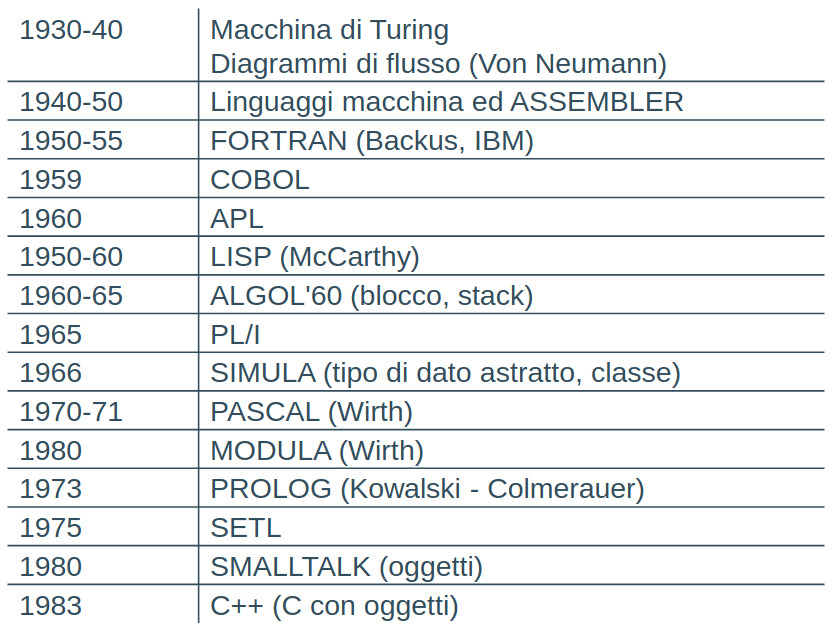
\includegraphics[width=1.00\textwidth]{linguaggi_programmazione}
	\end{figure}
	\section{Il linguaggio macchina}
	Descriviamo un semplice linguaggio che consente la programmazione di una macchina di von Neumann. \\
	Il linguaggio, volutamente "giocattolo", appartiene alla categoria dei linguaggi macchina cioè linguaggi direttamente eseguibili. \\
	Le istruzioni si dividono in due parti: un codice \textbf{operativo} (sempre presente) ed uno o più \textbf{operandi} (opzioni). \\
	Il codice operativo specifica l'operazione da compiere, mentre gli operandi le celle di memoria a cui si riferiscono le operazioni. Per semplicità, un solo operando. \\
	Anche le istruzioni sono inserite in memoria e quindi sono memorizzate in binario. \\
	\begin{figure}[H]
		\centering
		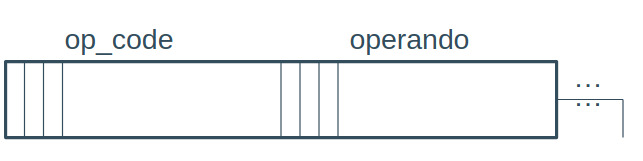
\includegraphics[width=0.4\textwidth]{formato_istruzioni}
	\end{figure}
	Il formato di un'istruzione è formato da due parti, il codice operativo e, per semplicità, un solo operando. \\
	Denotiamo con $s$ la lunghezza di un'istruzione in bit. $s = n + m$ ove $n$ è il numero di bit dedicati al codice operativo e $m$ il numero di bit dedicati all'indirizzamento degli operandi. \\
	Quindi, al più, ci saranno $2^n$ istruzioni diverse e $2^m$ celle di memoria indirizzabili. \\
	L'esecuzione di ogni istruzioni richiede tre fasi:
	\begin{enumerate}
		\item acquisizione dalla memoria centrale, la fase di \textbf{fetch};
		\item interpretazione del codice operativo, la fase di \textbf{decode};
		\item esecuzione, la fase di \textbf{execute}
	\end{enumerate}
	Le istruzioni principali sono le istruzioni di:
	\begin{enumerate}
		\item \textbf{LOAD}, caricamento di una cella di memoria in un opportuno registro ausiliario;
		\item \textbf{STORE}, carica il contenuto di un registro in una cella di memoria;
		\item \textbf{READ}, lettura da una periferica;
		\item \textbf{WRITE}, scrittura su una periferica;
		\item \textbf{Istruzioni numeriche:} ADD, DIF, MUL, DIV;
		\item \textbf{Istruzioni di salto incondizionato}, JUMP e modifica l'esecuzione sequenziale del programma;
		\item \textbf{Istruzione di salto condizionato}, JUMPZ effettua il salto solo se il contenuto di A (registro ausiliare) è zero;
		\item \textbf{NOP}, fa trascorrere un ciclo istruzione senza svolgere alcuna operazione;
		\item \textbf{HALT}, termina l'esecuzione del programma.
	\end{enumerate}
	Poichè sono 14 istruzioni, sono sufficienti 4 bit:
	\begin{figure}[H]
		\centering
		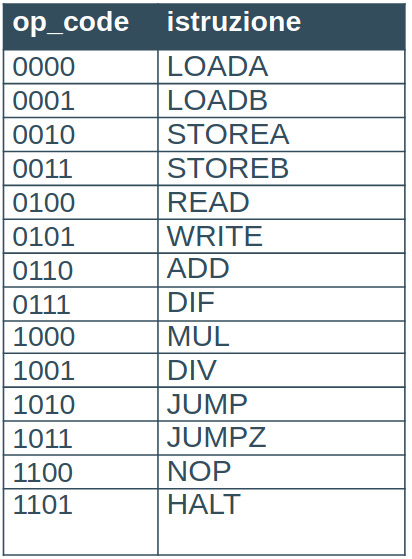
\includegraphics[width=0.6\textwidth]{esempio_istruzioni}
	\end{figure}
	Alcune macchine denominate RISC (Reduced Instruction Set Computer) sono caratterizzate dal disporre di un ridotto set di istruzioni con formati regolari eseguite in modo molto efficiente e hanno prestazioni migliori rispetto a macchine con molte istruzioni. \\
	Un programma consiste in due parti: istruzioni e dati. Per semplicità facciamo partire il programma dalla prima cella di memoria (loader). Poi seguono i dati. 
	\subsection{Il linguaggio ASSEMBLER}
	È difficile leggere e capire un programma scritto in forma binaria, per questo esistono i linguaggio di programmazione di alto livello che sono il più possibile indipendenti dalla macchina. \\
	Il primo passo sono i linguaggi assemblatori, dove le istruzioni corrispondono univocamente a quelle macchina, ma vengono espresse tramite parole chiave. I riferimenti alle celle di memoria sono fatti mediante nomi simbolici. IL programma prima di essere eseguito deve essere tradotto in linguaggio macchina per mezzo dell'\textbf{assemblatore}. \\
	\subsection{Linguaggi di alto livello}
	I linguaggi di alto livello sono simbolici ed indipendenti dalla macchina. Hanno costrutti "strutturati", per questo c'è maggiore flessibilità nello sviluppo e nel debugging. \\
	Questi linguaggi di programmazione richiedono opportuni "traduttori" e sono realizzati in termini di istruzione di basso libello, direttamente eseguite dal processore, attraverso l'interpretazione o la compilazione. \\
	I \textbf{compilatori} traducono un programma dal linguaggio $L$ a quello macchina. \\
	Gli \textbf{interpreti} sono programmi capaci di eseguire direttamente un programma in linguaggio L istruzione per istruzione. \\
	I programmi compilati sono in generale più efficienti di quelli interpretati. \\
	Il \textbf{compile-time} è il momento in cui avviene la conversione da programma sorgente a programma oggetto. Il \textbf{run-time} è il momento in cui viene eseguito il programma oggetto.
	\paragraph{Approccio compilato} \quad \\
	\begin{figure}[H]
		\centering
		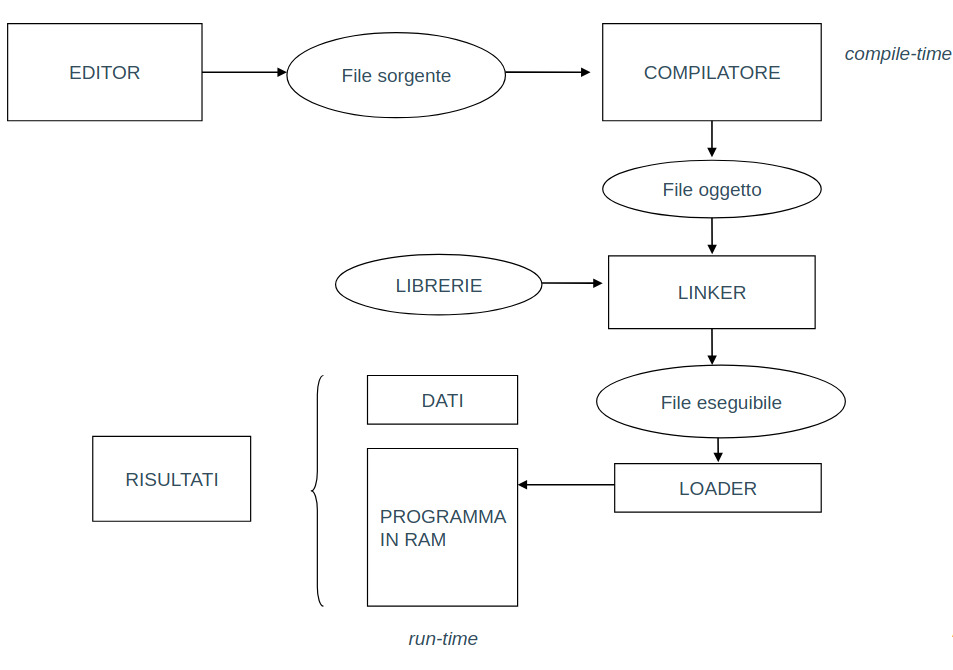
\includegraphics[width=1.0\textwidth]{approccio_compilato}
	\end{figure}
	\paragraph{Approccio interpretato} \quad \\
	\begin{figure}[H]
		\centering
		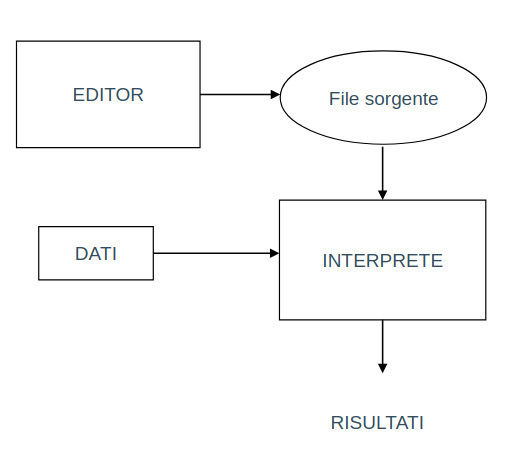
\includegraphics[width=0.5\textwidth]{approccio_interpretato}
	\end{figure}
	Nell'approccio interpretato, invece, l'interprete processa una forma intera del programma sorgente ed i dati nello stesso momento e non genera quindi nessun codice oggetto. \\
	Alcuni interpreti analizzano ogni istruzione del programma sorgente ogni volta che viene eseguita. È ovviamente un approccio molto dispendioso. Un approccio più efficiente consiste nell'applicare tecniche di compilazione per produrre un codice intermedio che viene poi interpretato dall'utente.
	\section{Semantica di un linguaggio di programmazione}
	Essa attribuisce un significato ai costrutti linguistici del linguaggio e molto spesso non è definita formalmente. \\
	\textbf{Metodi formali}:
	\begin{itemize}
		\item\textbf{semantica operazionale}, tramite le azioni;
		\item \textbf{semantica denotazionale}, tramite funzioni matematiche;
		\item \textbf{semantica assiomatica} tramite formule logiche.
	\end{itemize}
	Ci sono benefici per il programmatore (comprensione dei costrutti, prove formali di correttezza), l'implementatore (costruzione del traduttore corretto), progettista di linguaggi (strumenti formali di progetto). \\
	\subsection{Metodo operazionale}
	Definire una semantica operazionale per un linguaggio di programmazione L significa definire una macchina astratta e definire come l'esecuzione delle istruzioni di L viene condotta su tale macchina. \\
	La macchina astratta è caratterizzata da uno \textbf{stato}. La semantica di ciascun costrutto è data in termini di \textbf{transizioni di stato}. Il \textbf{significato di un programma} è rappresentato dalla \textbf{sequenza di stati} che la macchina astratta attraversa durante l'esecuzione. \\
	Il \textbf{vantaggio} è che ci si basa solo sul programma. \\
	(Vedere esempi dalle slide).
	\subsection{Metodo denotazionale}
	Definire una semantica denotazionale significa fornire un metodo rigoroso per associare ad ogni programma del linguaggio L la \textbf{funzione calcolata dal programma}. \\
	Programma P che termina sull'ingresso $i$ e produce l'output $o$.
	\[
	fp:\ fp(i) = o
	\]
	$fp$ viene determinata risolvendo un insieme di equazioni funzionali. \\
	Studiando $fp$ si ricavano proprietà sul programma $P$.
	\section{Metodo assiomatico (Hoare)}
	Definire una semantica assiomatica significa fornire un metodo rigoroso per associare ad ogni programma del linguaggio L la \textbf{relazione calcolata dal programma} (formula logica). \\
	Programma P che termina sull'ingresso $i$ e produce l'output $o$:
	\[
	Rp:\ Rp(i, o)
	\]
	$Rp$ viene generalmente espressa nel calcolo dei predicati. \\
	Il metodo assiomatico lega \textbf{pre- e post-condizione}:
	\begin{figure}[H]
		\centering
		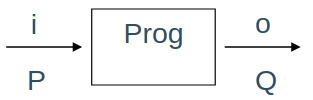
\includegraphics[width=0.4\textwidth]{metodo_assiomatico}
	\end{figure}
	Se la precondizione $P$ è vera sui dati di ingresso $i$ ed il programma $Prog$ termina, allora la postcondizione è vera sui dati di uscita $o$. \\
	Semantica assiomatica di $Prog$, coppia $P, Q$ tale che vale l'espressione:
	\[
	\{P\}\ Prog\ \{Q\}
	\]
	L'esecuzione di $Prog$ in uno stato che soddisfa $P$ porta ad uno stato che soddisfa $Q$. \\
	Per ciascuna istruzione del linguaggio occorre definire come sono correlate pre- e post-condizioni. \\
	Specificato attraverso \textbf{assiomi} o \textbf{regole di inferenza}. \\
	Pre- e post-condizione, situazione della memoria prima e dopo l'esecuzione dell'istruzione. \\
	\textbf{Operazione e semantica associata}:
	\[
	\{P\}\  readln(n)\ \{P\ [i/n]\}
	\]
	\[
	\{P\}\ writeln(n)\ \{P\}
	\]
	\[
	\{P\}\ n:=exp\ \{P\ [v/n]\}
	\]
	dove $v$ è il valore risultante dalla valutazione di exp.
	\begin{figure}[H]
		\centering
		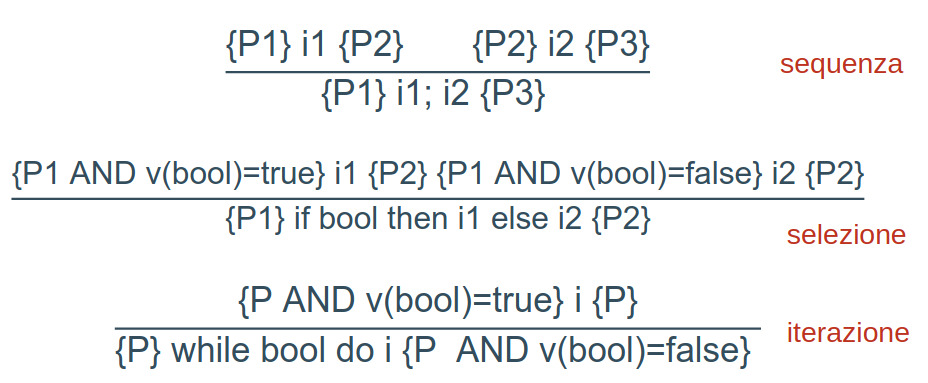
\includegraphics[width=1.00\textwidth]{es_metodi_assiomatici}
	\end{figure}
	Se $P$ è vera prima di eseguire l'istruzione while e questa termina, $P$ è vera anche dopo e a questo punto bool ha valore falso.
	\[
	P\ \textbf{invariante del ciclo}
	\]
	Il metodo assiomatico viene utilizzato per eseguire \textbf{prove formali} della correttezza di un programma. \\
	Dimostrare che $Prog$ è corretto rispetto alle condizioni $P, Q$ significa dimostrare che l'espressione:
	\[
	\{P\}\ Prog\ \{Q\}
	\]
	è soddisfatta usando assiomi e regole di inferenza che definiscono la semantica del linguaggio. \\
	\section{Analisi di programmi: la correttezza}
	Oltre il 50\% del costo di un progetto software è dovuto alla prova (test) ed alla correzione del programma. \\
	\textbf{Tipologie di errori:}
	\begin{itemize}
		\item \textbf{Errori nell'uso del linguaggio}:
		\begin{itemize}
			\item lessicali;
			\item sintattici;
			\item semantici.
		\end{itemize}
		\item \textbf{Errori logici}: sono dovuti ad una scelta sbagliata dell'algoritmo o delle strutture dati.
		\item \textbf{Errori di codifica}: ad esempio, errore condizione booleana di un ciclo while.
	\end{itemize}
	Problema, A
	\begin{figure}[H]
		\centering
		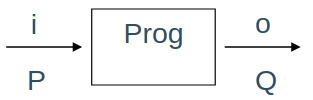
\includegraphics[width=0.4\textwidth]{metodo_assiomatico}
	\end{figure}
	Perchè $Prog$ possa essere utilizzato correttamente i dati di ingresso devono soddisfare la condizione P (vincoli sull'input). \\
	$Prog$ risolve correttamente il problema se l'output soddisfa il vincolo $Q$. \\
	$\{P\}\ Prog\ \{Q\}$ \textbf{specifica}. \\
	La specifica è soddisfatta se per ogni insieme dei dati di ingresso che soddisfa P, $Prog$ termina ed i dati di uscita soddisfano Q. Si dice che $Prog$ è corretto.
	\subsection{Prove formali di correttezza}
	\begin{enumerate}
		\item Si determinano P e Q (pre-, post-condizione)
		\item Si verifica se la specifica $\{P\}\ Prog\ \{Q\}$ è soddisfatta. 
		\item Si stabilisce se $Prog$ termina con ogni configurazione dei dati di ingresso che soddisfa P.
	\end{enumerate}
	Facilitata dall'uso sistematico della programmazione strutturata (un ingresso ed una uscita).
	\subsection{Correttezza: un metodo più pragmatico}
	Si parla di \textit{test} di un programma.
	\begin{enumerate}
		\item Si determina un insieme di dati di ingresso I;
		\item Si esegue il programma con i dati I;
		\item Si verificano i risultati ottenuti:
		\begin{enumerate}
			\item Se l'esecuzione non termina in un tempo ragionevole oppure i risultati non sono quelli attesi, programma non corretto;
			\item se non sono stati rilevati errori, ma si vogliono effettuare altre prove si torna al passo 1. Altrimenti il test termina.			
		\end{enumerate}
	\end{enumerate}
	Il test di un programma non permette di stabilire la correttezza, a meno di non provare con tutti i possibili dati di ingresso. \\
	È tuttavia il metodo più usato in pratica per rilevare errori.
	\paragraph{Strategie per effettuare il test} \quad \\
	I metodi per il test di un programma si classificano in:
	\begin{itemize}
		\item \textbf{metodi basati sulle specifiche del programma} o a scatola nera:
		\begin{itemize}
			\item esecuzione con diversi dati di ingresso;
			\item gli infiniti dati di ingresso sono suddivisi in \textbf{classi di equivalenza}: per ciascuna classe si programma con almeno un elemento di ingresso.
			\item Trade-off: pochi o molti insieme di equivalenza
		\end{itemize}
		\item \textbf{metodi basati sulla struttura del programma} o a scatola trasparente:
		\begin{itemize}
			\item diverse esecuzioni in modo da provare tutte le parti (istruzioni) del programma (\textbf{copertura del programma}).
		\end{itemize}
	\end{itemize}
	\subsection{Debugging}
	L'individuazione di un errore (debugging) è necessaria per poterlo correggere. \\
	È spesso difficile localizzare l'errore (si conosce il sintomo, ma non l'istruzione che ne è la causa). \\
	\textbf{Diagnosi di programmi}: Si ipotizza che l'errore sia in una certa parte del programma e si cerca di avere il massimo di informazione sulle variabili usate in quella parte del programma. \\
	Ipotesi di errore e verifica se dopo la correzione il malfunzionamento è scomparso. \\
	Esistono debugger integrati che consentono di eseguire un programma una riga alla volta (tracing), tenendo contemporaneamente sotto controllo i valori delle variabili (finestra di watching). Altrimenti si utilizza il \textbf{metodo delle stampe}.
\end{document}
